\documentclass{article}
\usepackage{amsmath}
\usepackage{graphicx}

\begin{document}

%\begin{table}[htbp]
%  \caption{Table of the experiments performed}
%\documentclass{article}
\usepackage{amsmath}
\usepackage{graphicx}

\begin{document}

%\begin{table}[htbp]
%  \caption{Table of the experiments performed}
%\documentclass{article}
\usepackage{amsmath}
\usepackage{graphicx}

\begin{document}

%\begin{table}[htbp]
%  \caption{Table of the experiments performed}
%\documentclass{article}
\usepackage{amsmath}
\usepackage{graphicx}

\begin{document}

%\begin{table}[htbp]
%  \caption{Table of the experiments performed}
%\input{barry.tex}
%\end{table}

\section{Numerical results for speed}


\begin{figure}[htbp]
\centering
  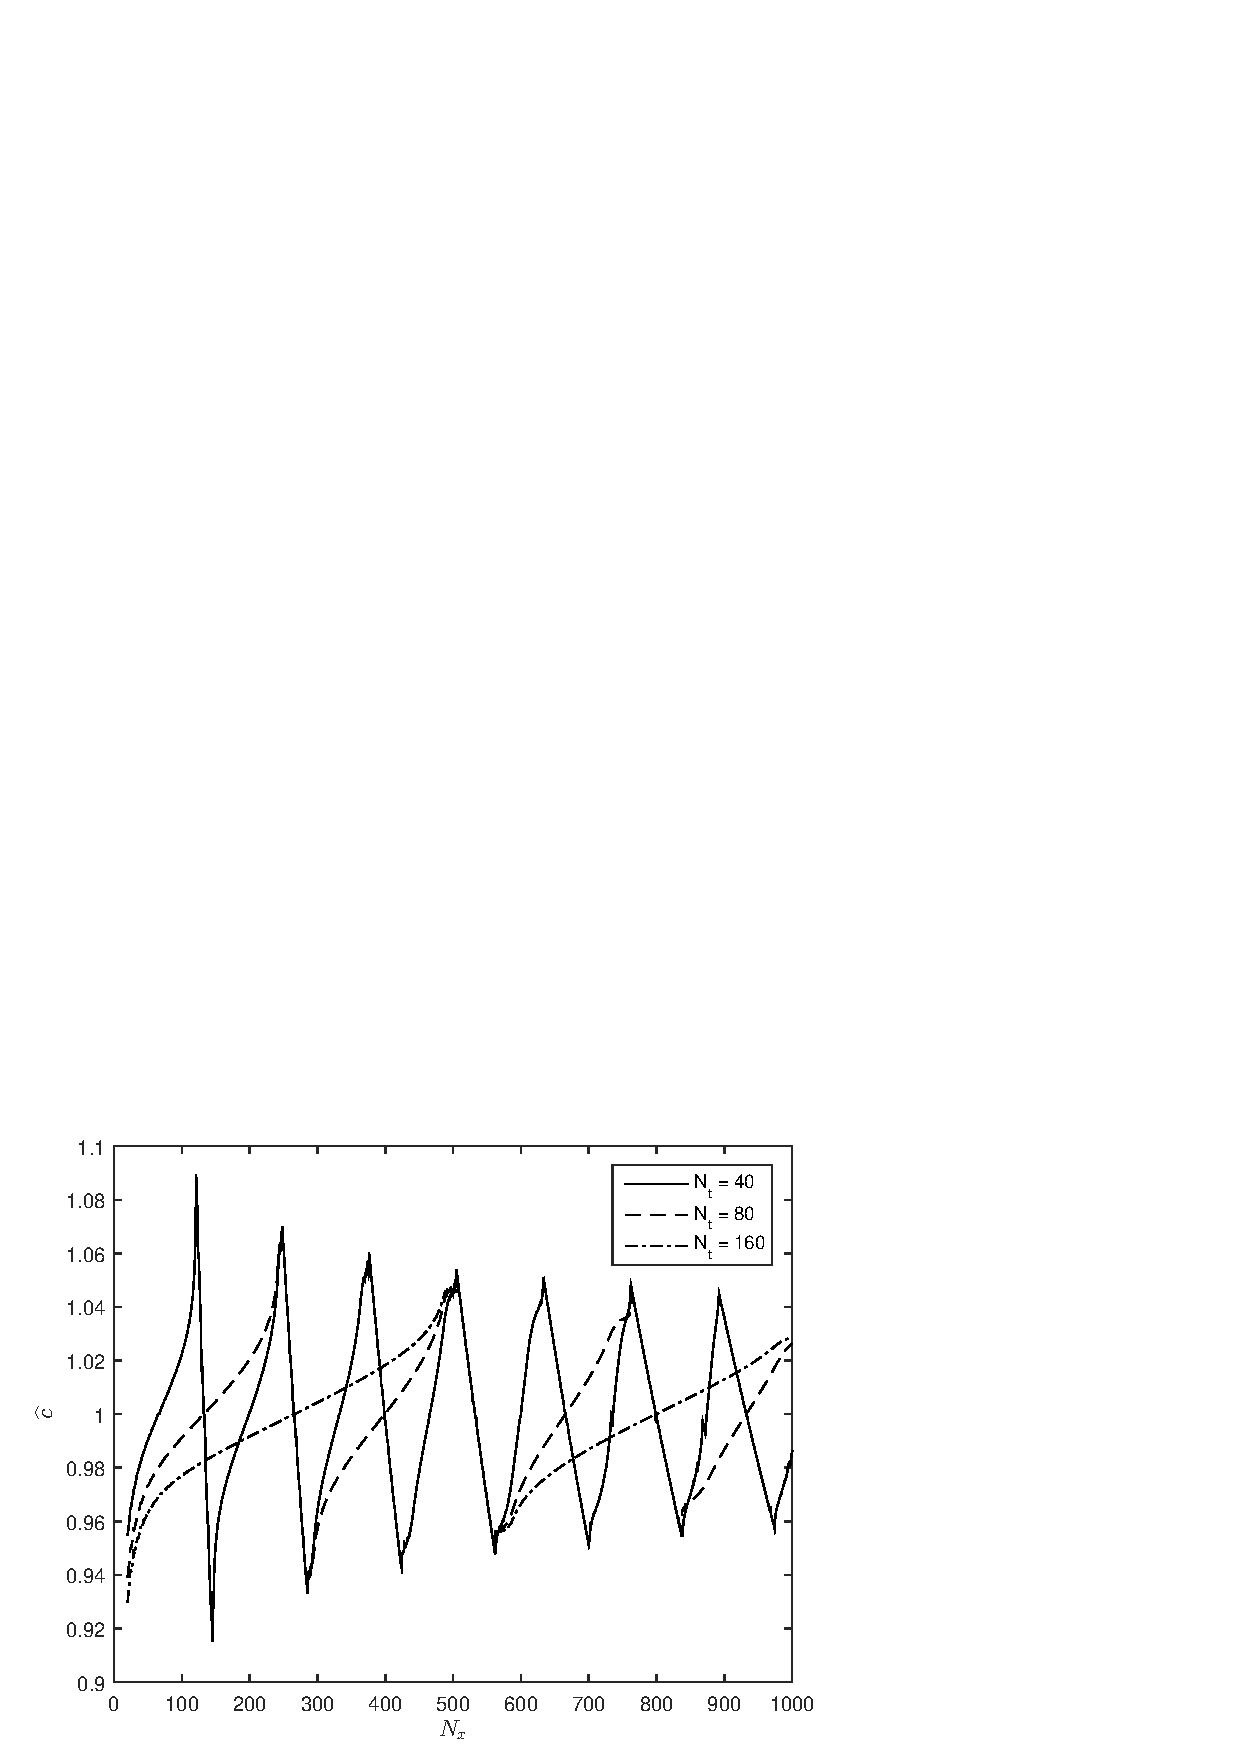
\includegraphics[width=0.9\textwidth]{barry1-k.pdf}
  \caption{Hermite interpolant with Hyman derivative estimates and guaranteed
    monotonicity.
  \label{fig:barry1-k}}
\end{figure}
\begin{figure}[htbp]
\centering
  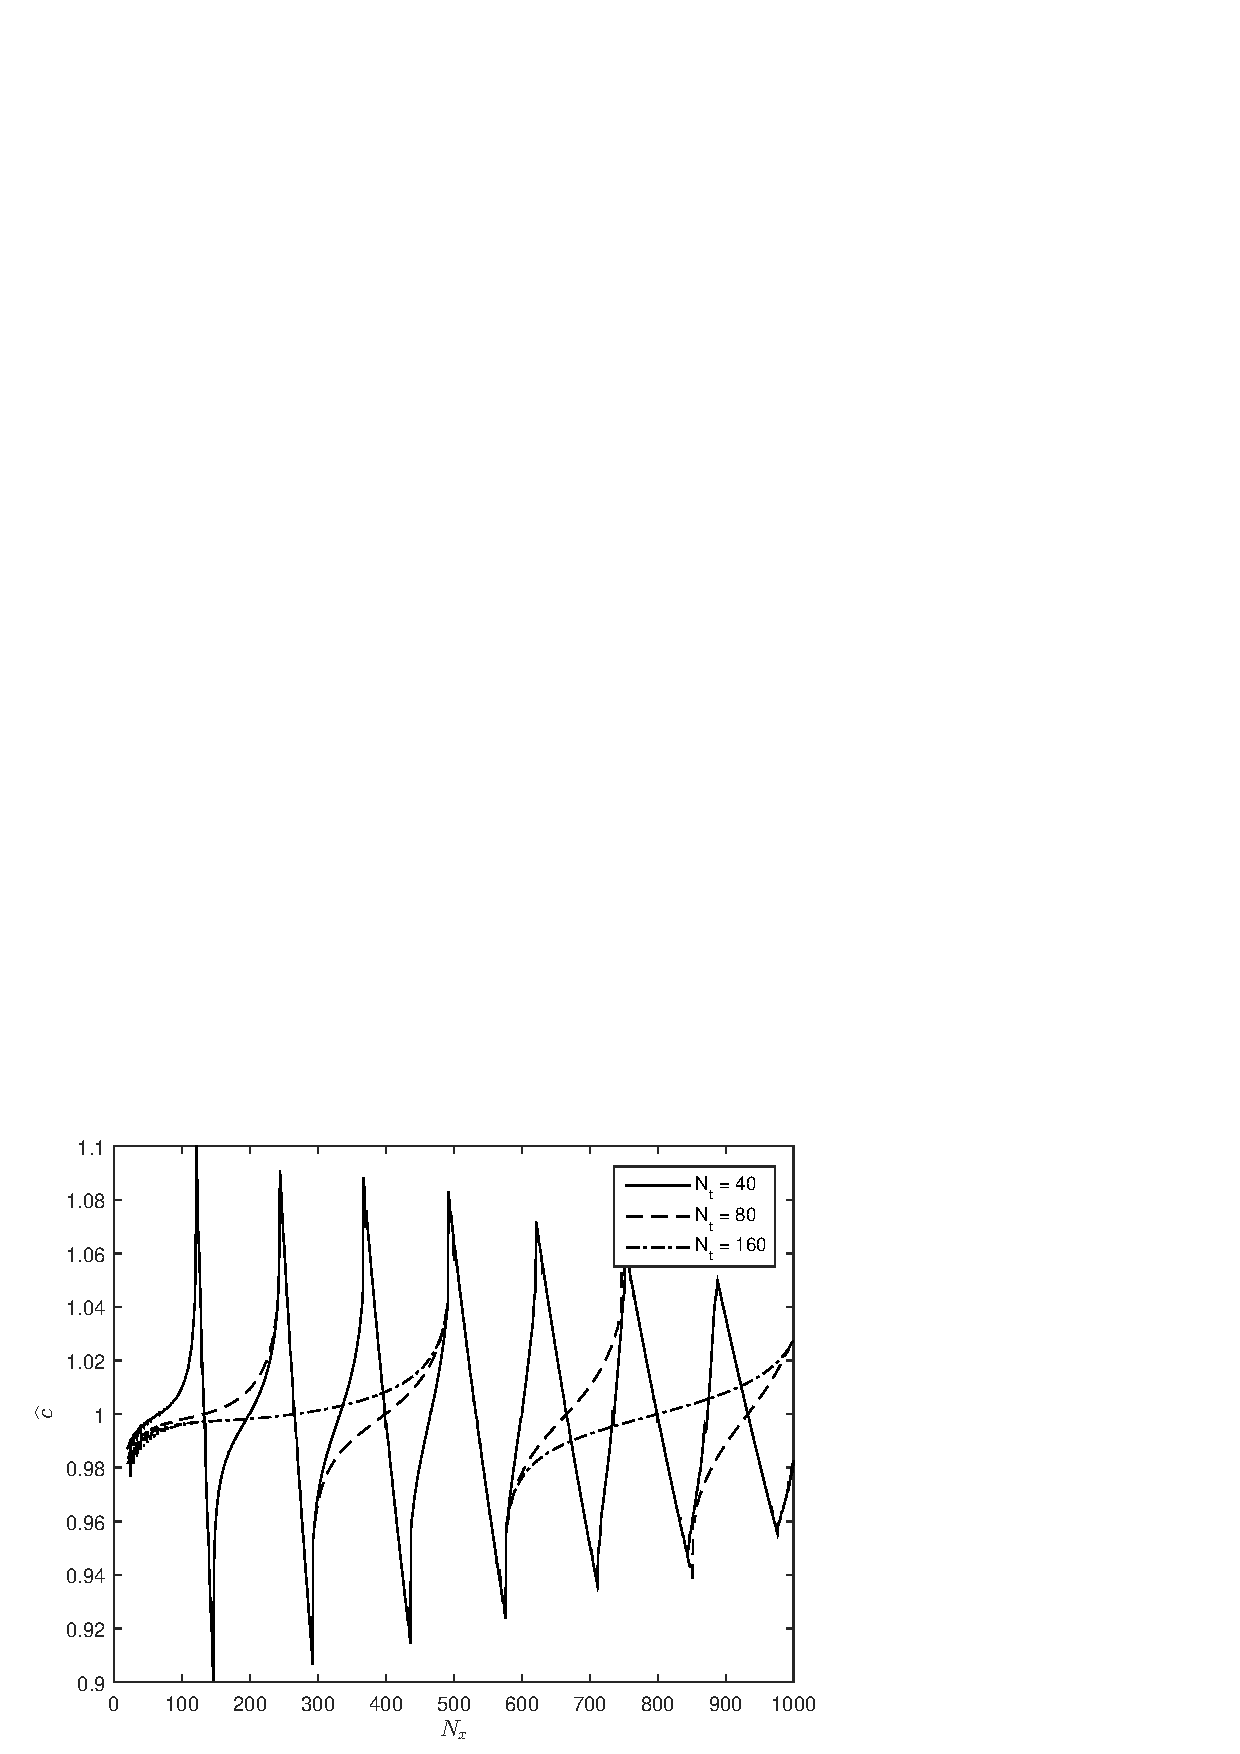
\includegraphics[width=0.9\textwidth]{barry2-k.pdf}
  \caption{Hermite interpolant with Hyman derivative estimates.
  \label{fig:barry2-k}}
\end{figure}
\begin{figure}[htbp]
\centering
  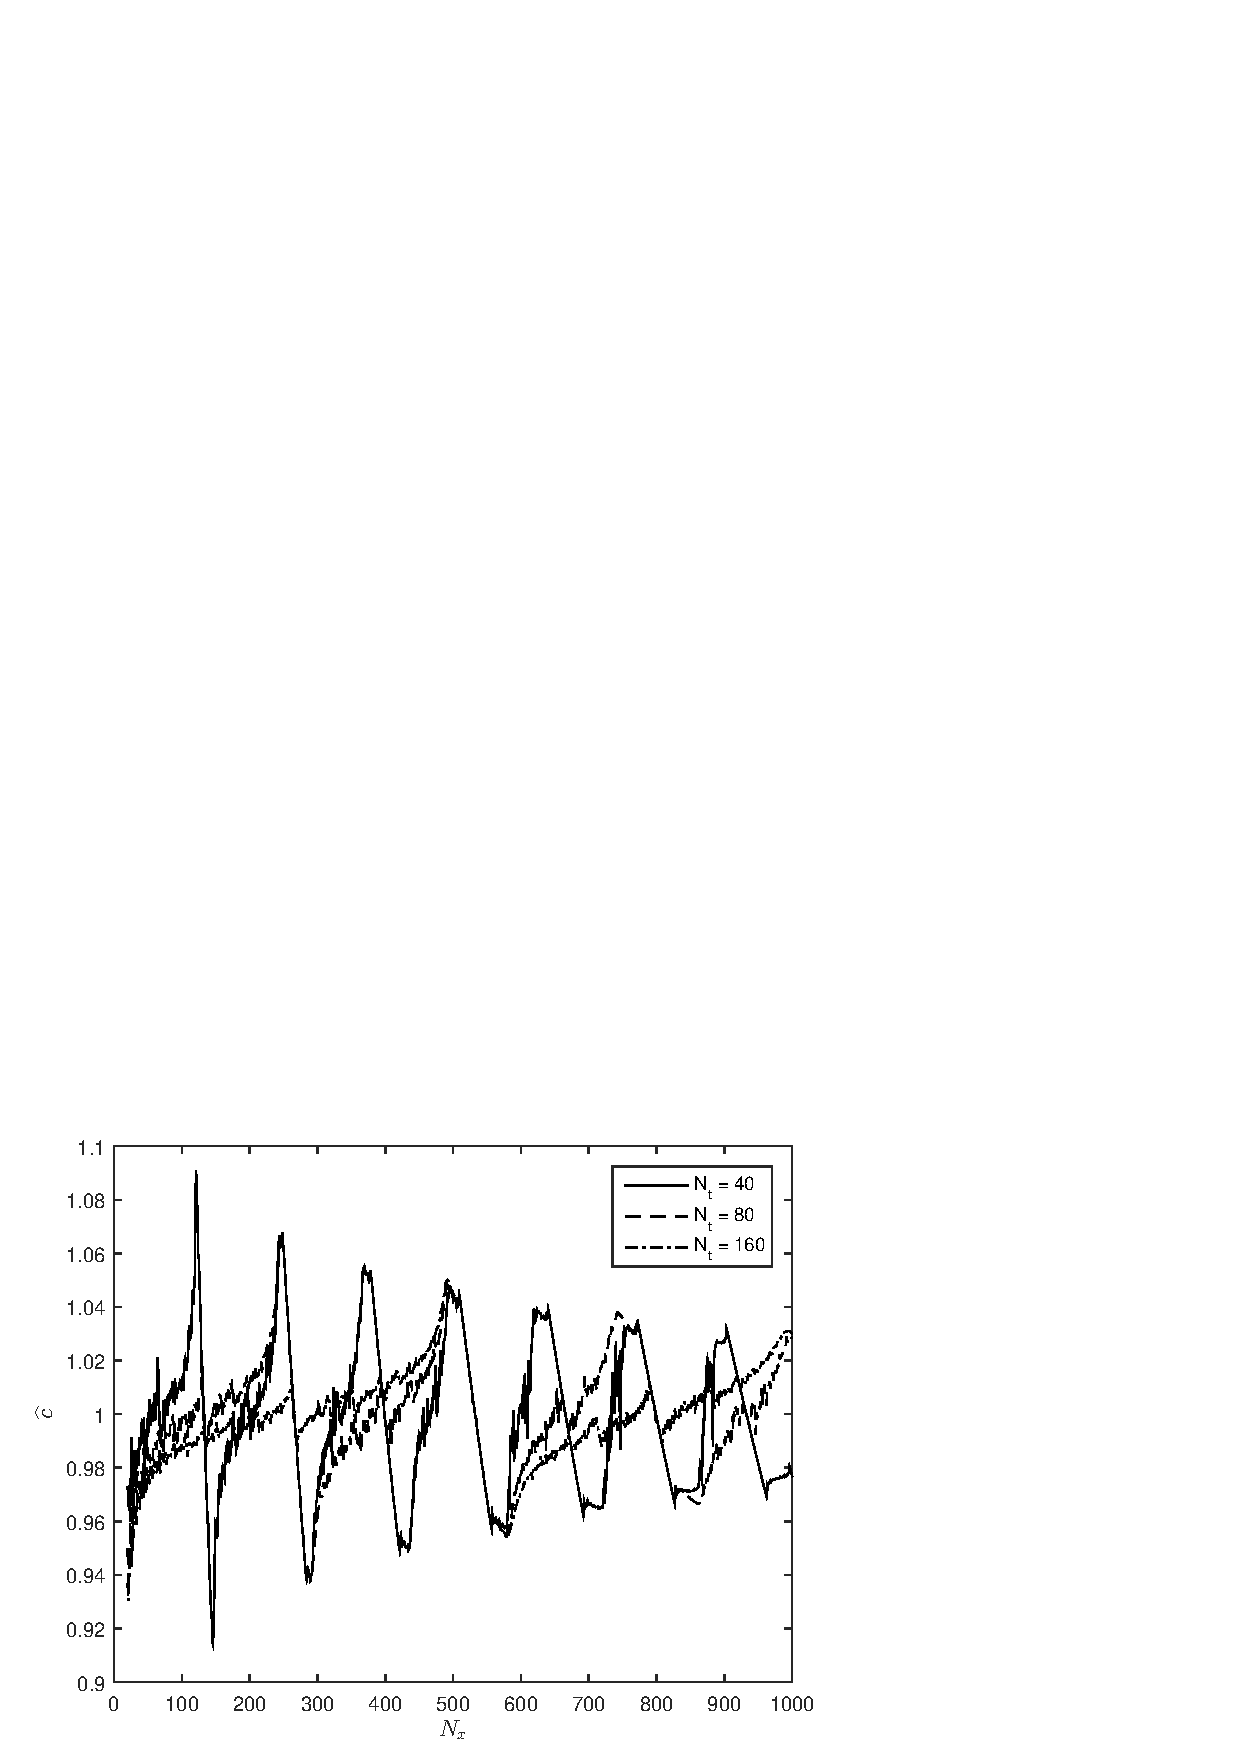
\includegraphics[width=0.9\textwidth]{barry3-k.pdf}
  \caption{ENO interpolant, followed by a flux limiter.
  \label{fig:barry3-k}}
\end{figure}
\begin{figure}[htbp]
\centering
  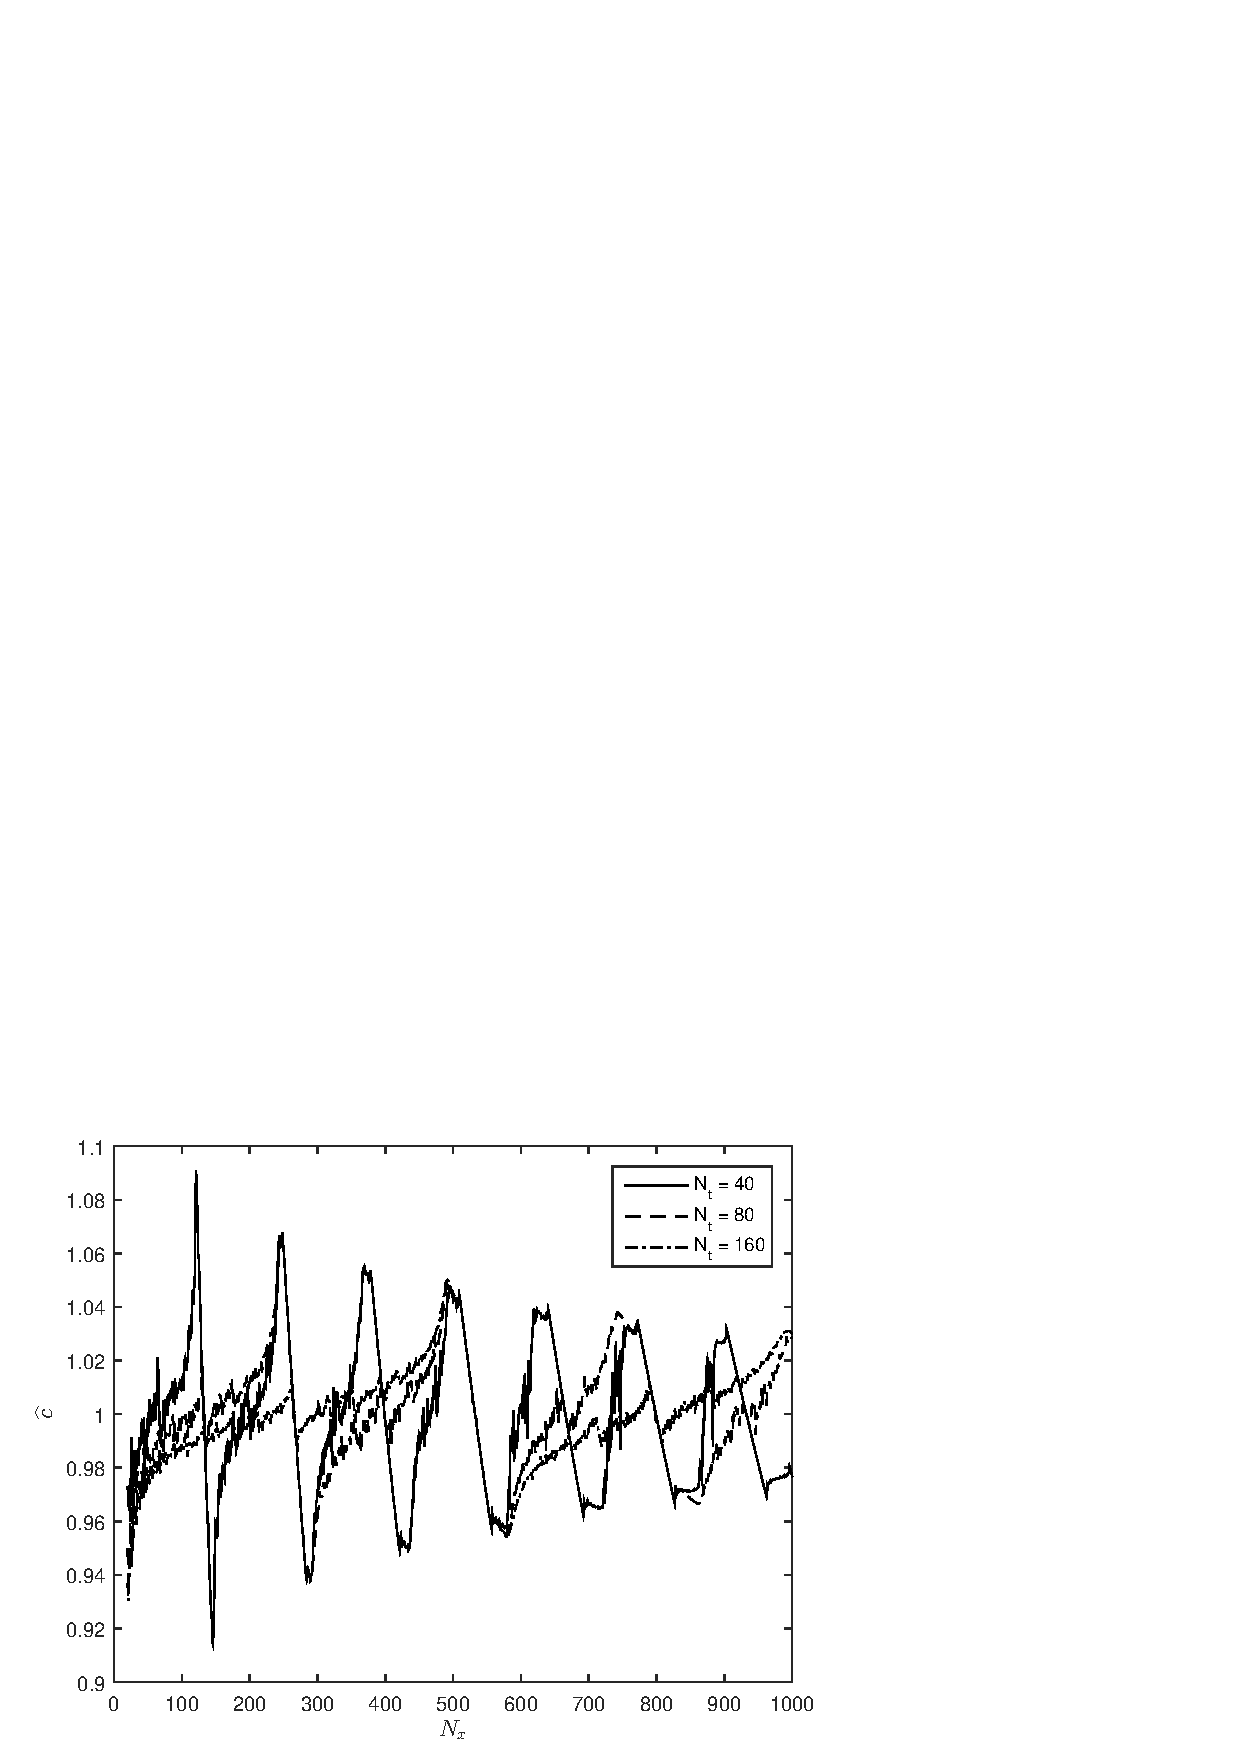
\includegraphics[width=0.9\textwidth]{barry4-k.pdf}
  \caption{ENO interpolant, no flux limiter.
  \label{fig:barry4-k}}
\end{figure}

\clearpage
\section{Numerical results for viscosity}

\begin{figure}[htbp]
\centering
  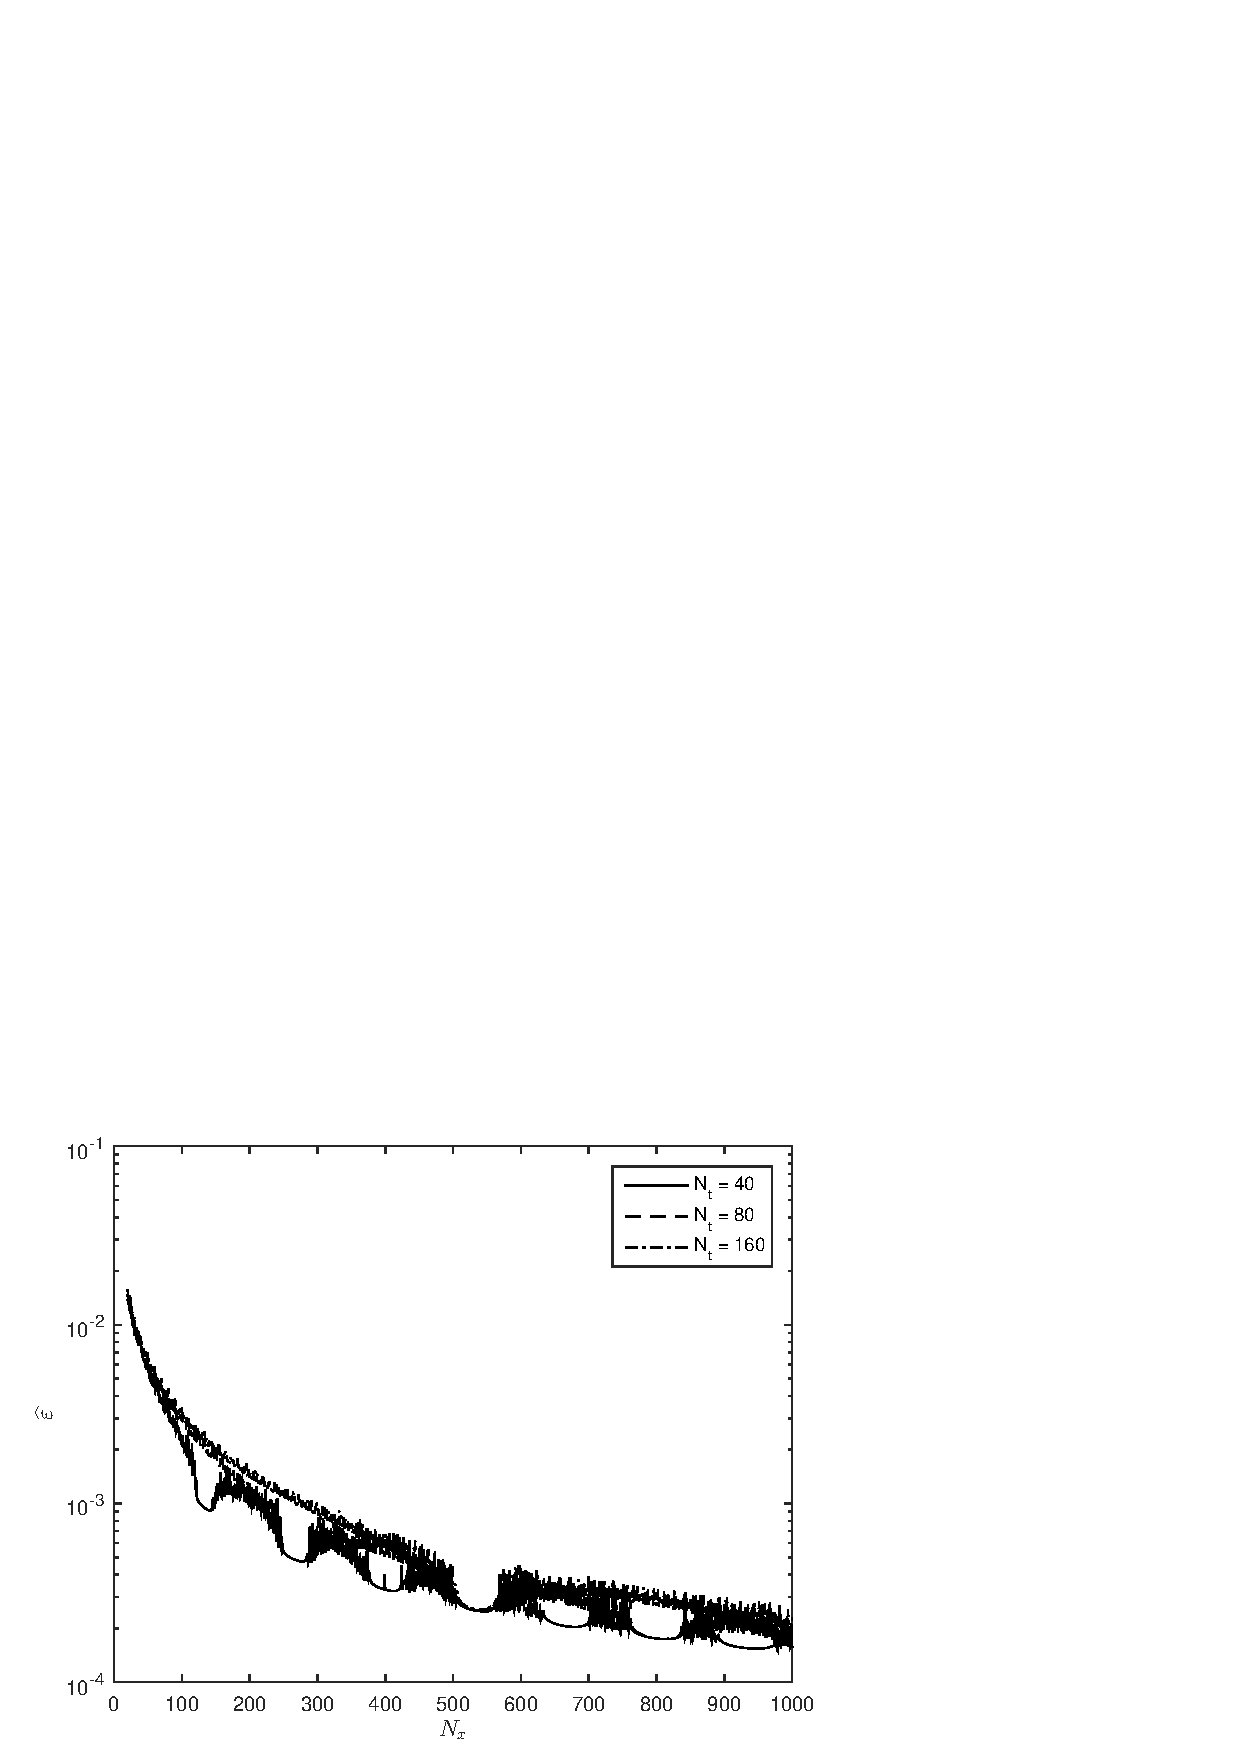
\includegraphics[width=0.9\textwidth]{barry1-eps.pdf}
  \caption{Hermite interpolant with Hyman derivative estimates and guaranteed
    monotonicity.
  \label{fig:barry1-eps}}
\end{figure}
\begin{figure}[htbp]
\centering
  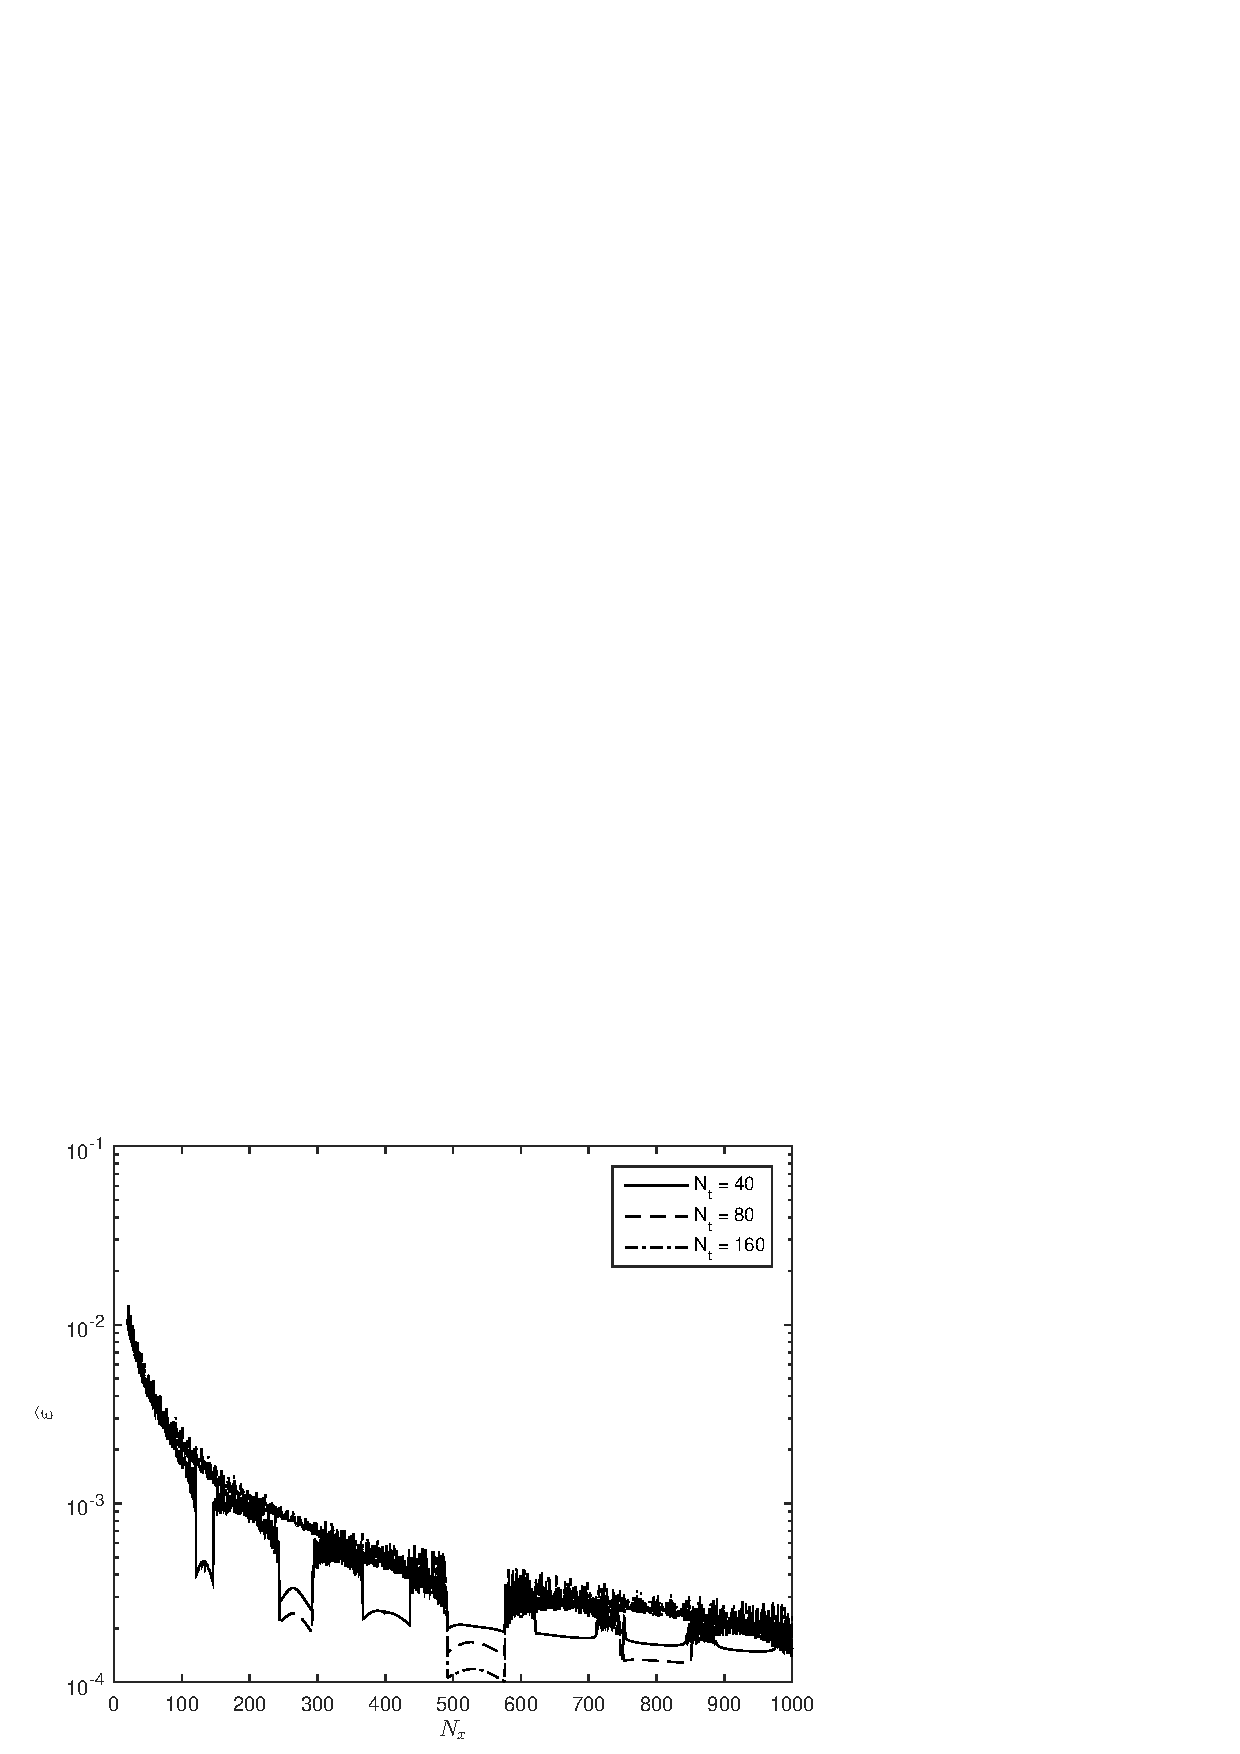
\includegraphics[width=0.9\textwidth]{barry2-eps.pdf}
  \caption{Hermite interpolant with Hyman derivative estimates.
  \label{fig:barry2-eps}}
\end{figure}
\begin{figure}[htbp]
\centering
  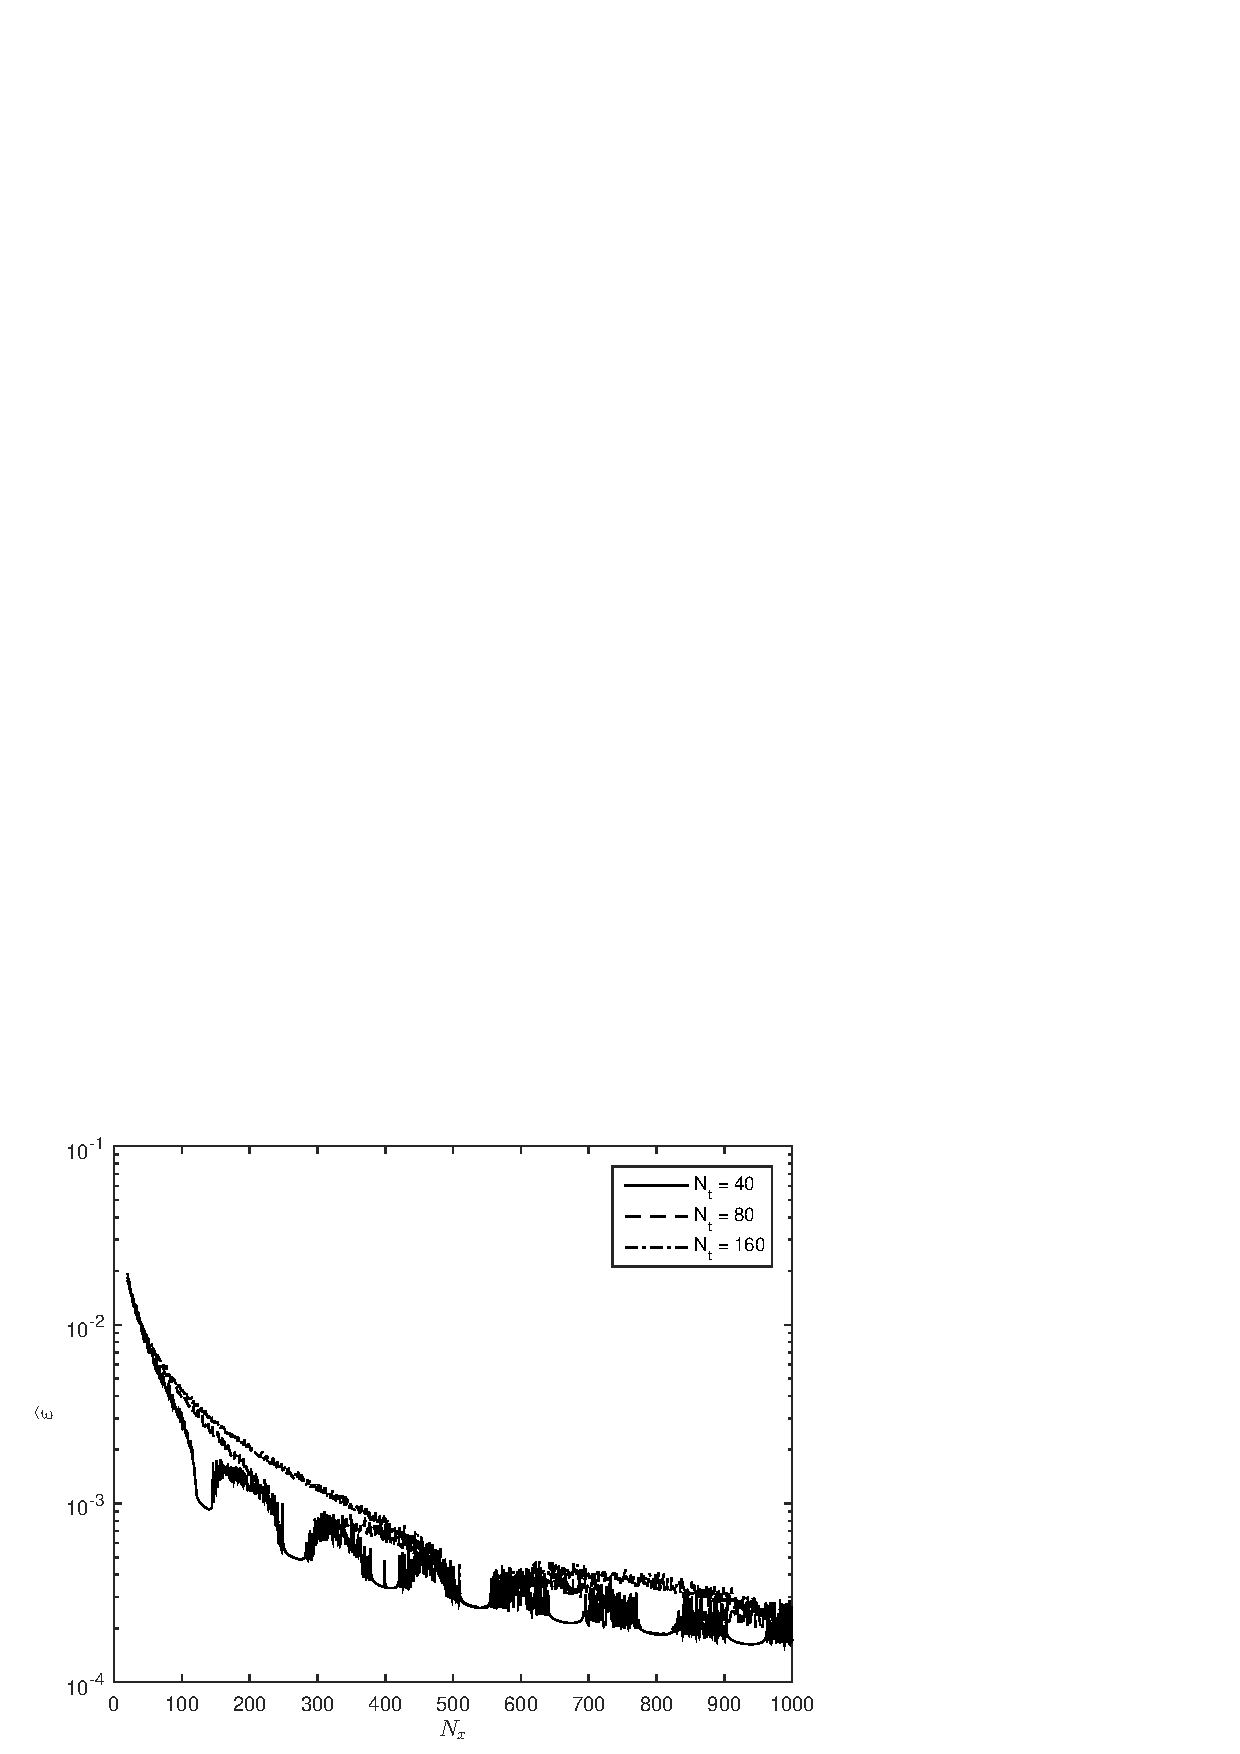
\includegraphics[width=0.9\textwidth]{barry3-eps.pdf}
  \caption{ENO interpolant, followed by a flux limiter.
  \label{fig:barry3-eps}}
\end{figure}
\begin{figure}[htbp]
\centering
  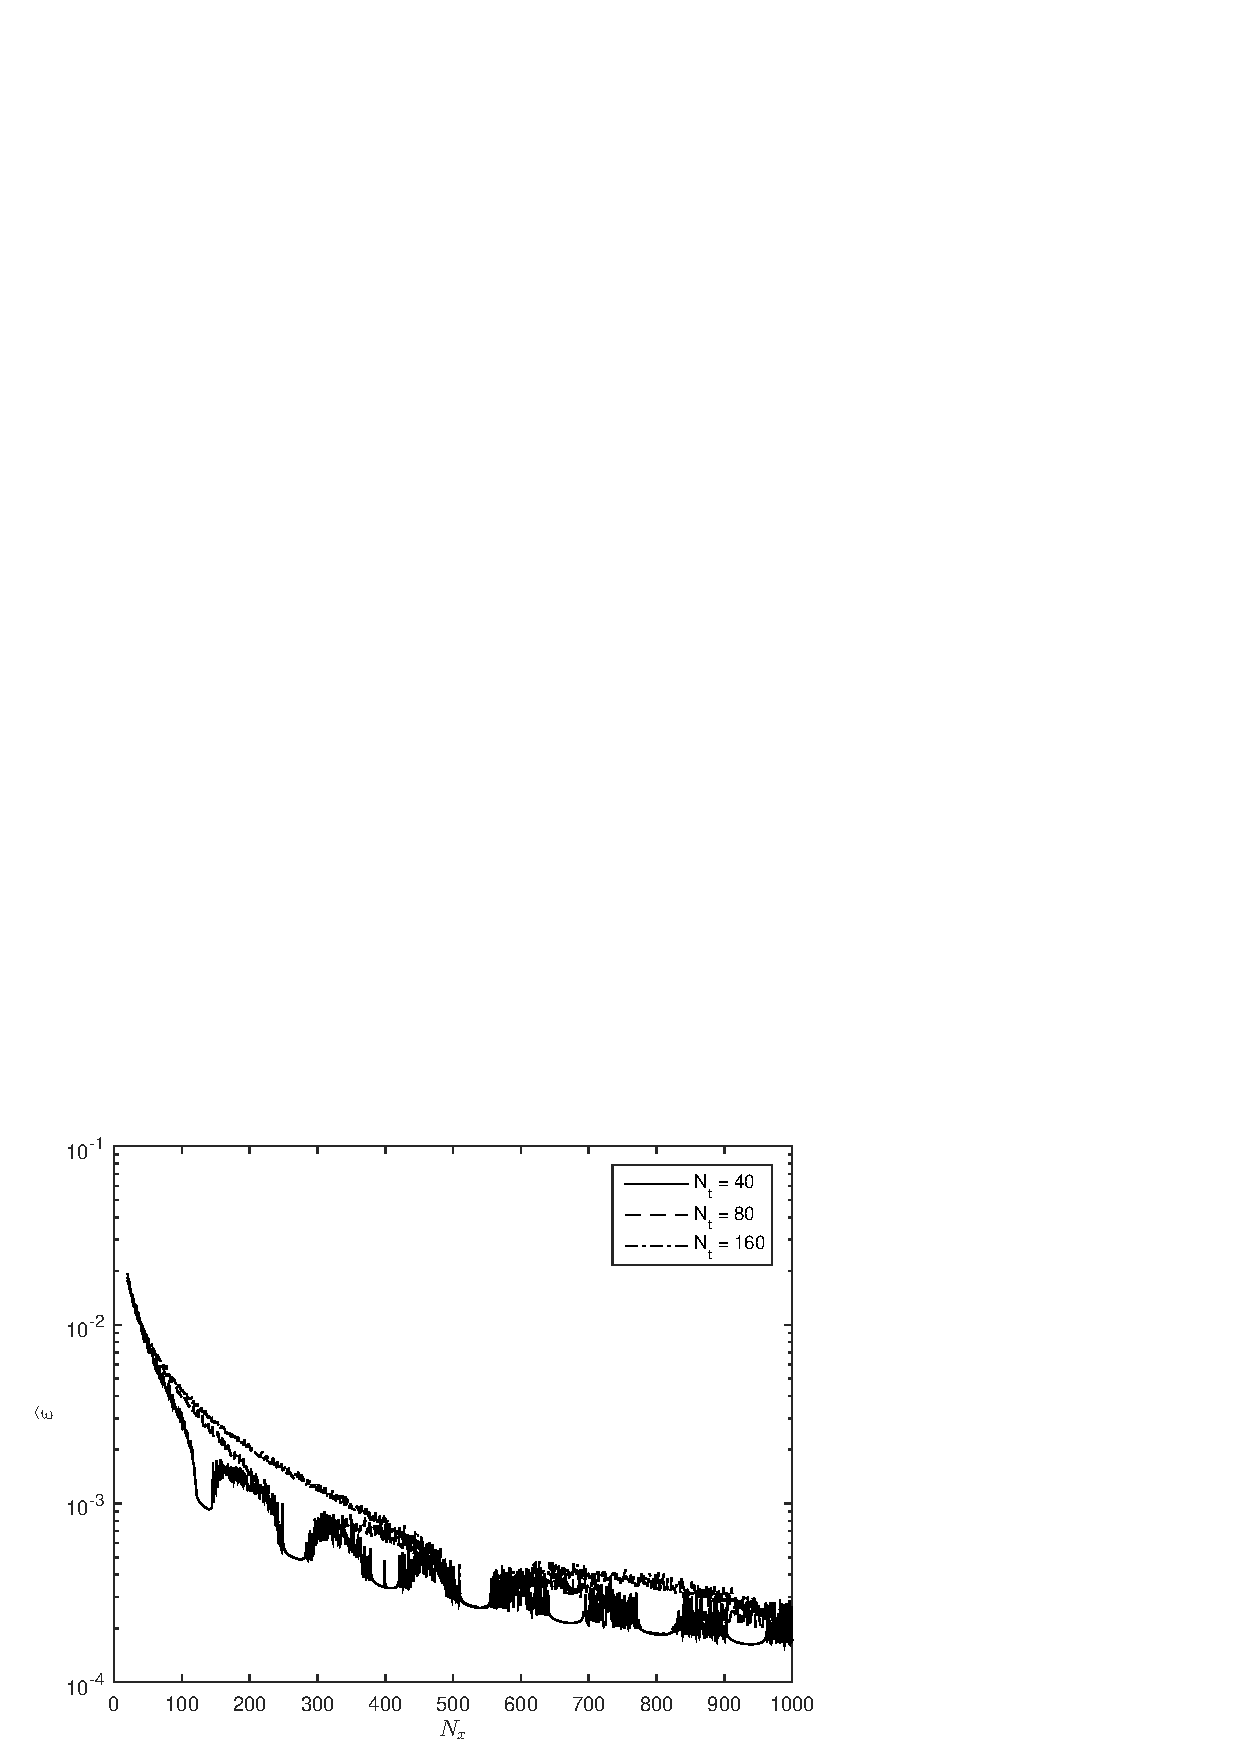
\includegraphics[width=0.9\textwidth]{barry4-eps.pdf}
  \caption{ENO interpolant, no flux limiter.
  \label{fig:barry4-eps}}
\end{figure}

\end{document}

%\end{table}

\section{Numerical results for speed}


\begin{figure}[htbp]
\centering
  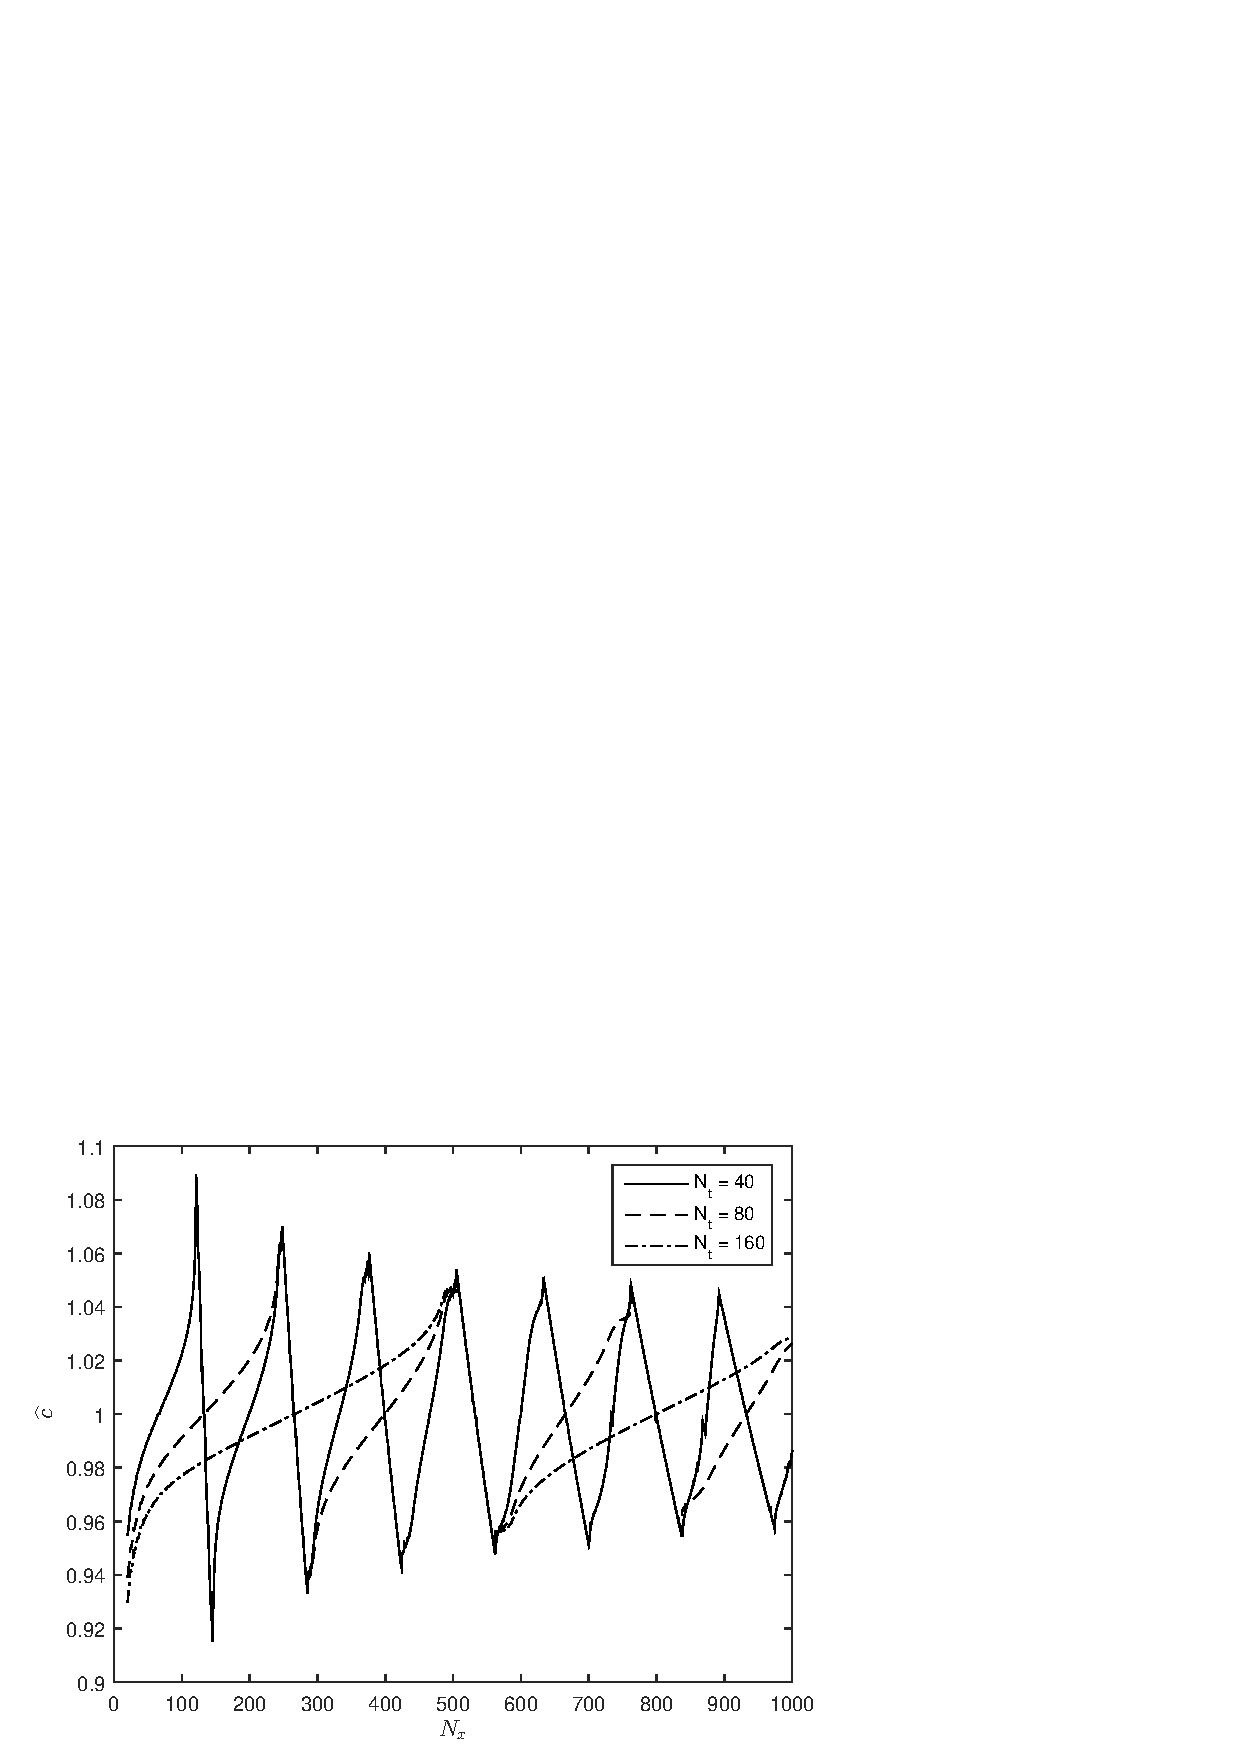
\includegraphics[width=0.9\textwidth]{barry1-k.pdf}
  \caption{Hermite interpolant with Hyman derivative estimates and guaranteed
    monotonicity.
  \label{fig:barry1-k}}
\end{figure}
\begin{figure}[htbp]
\centering
  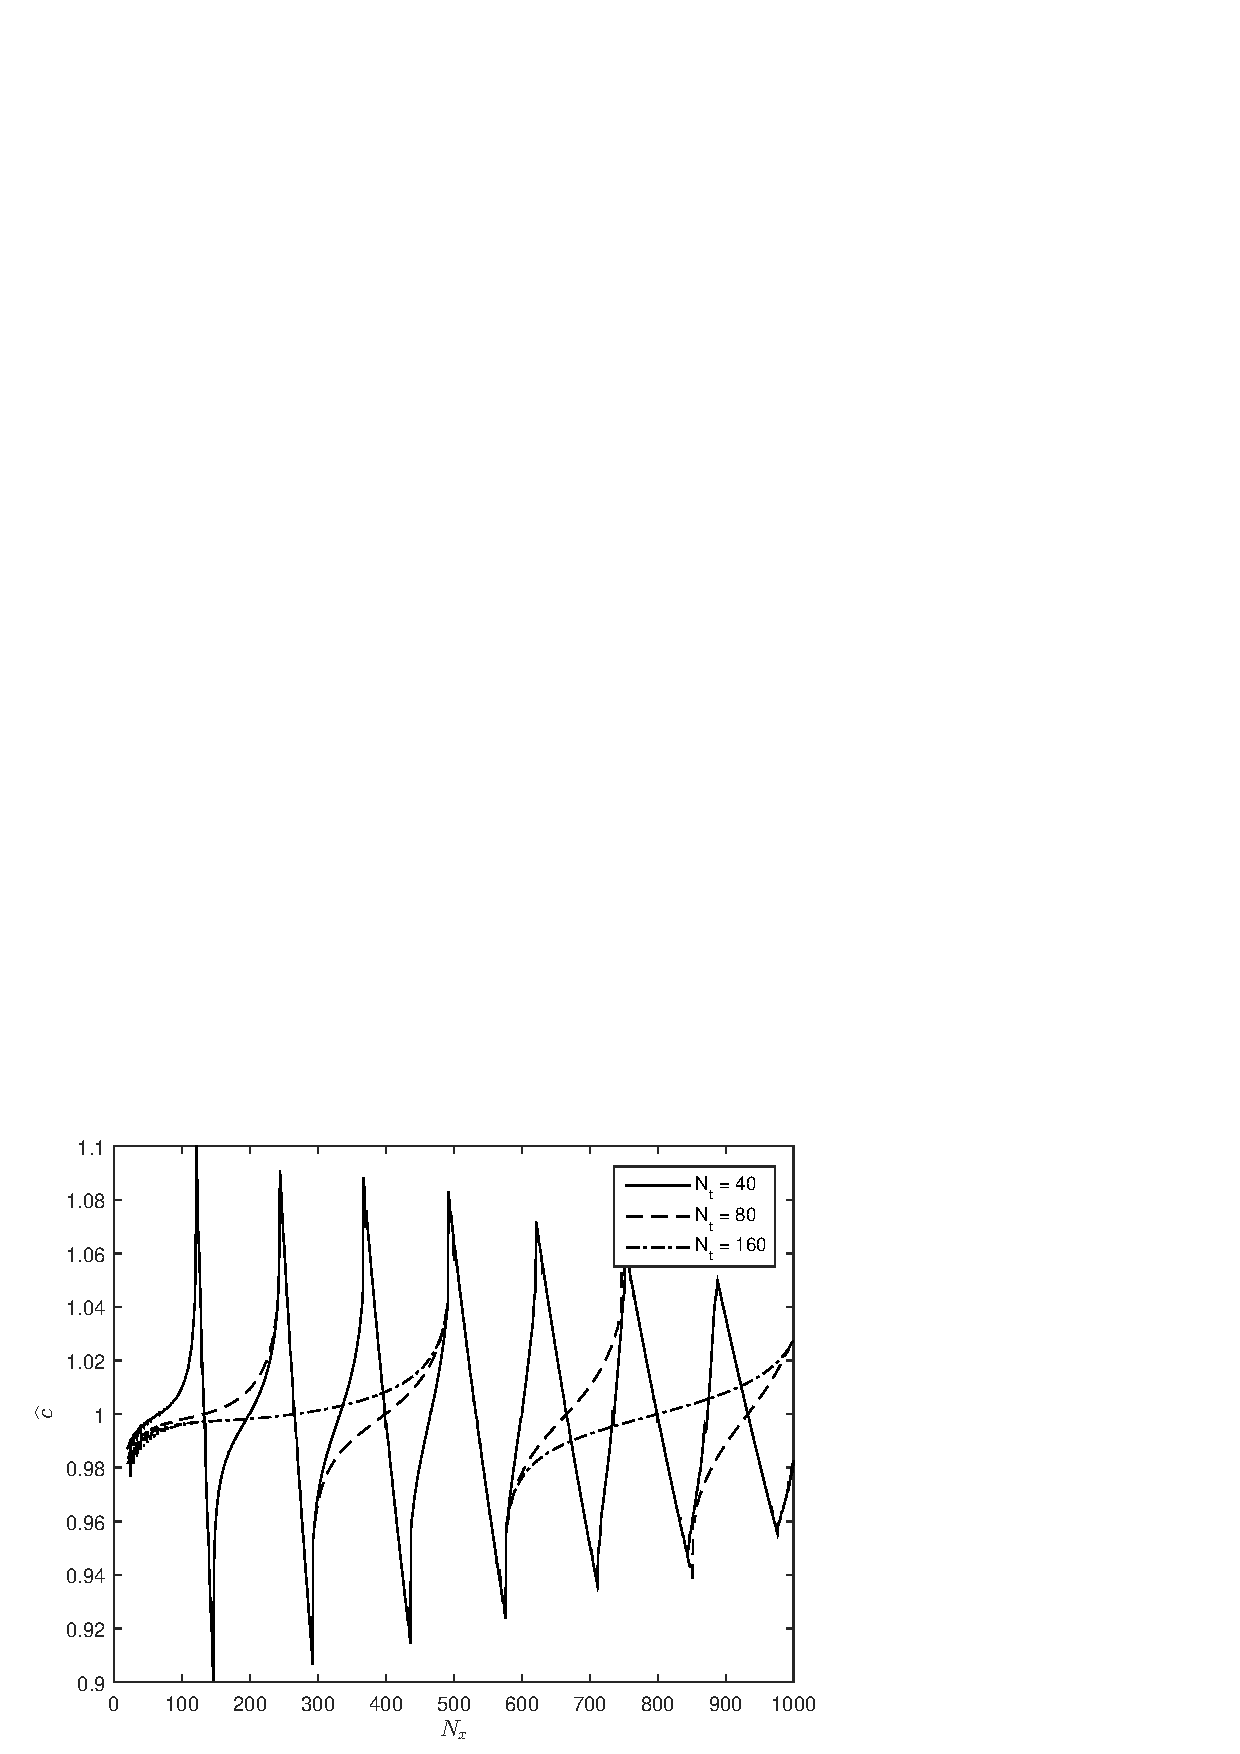
\includegraphics[width=0.9\textwidth]{barry2-k.pdf}
  \caption{Hermite interpolant with Hyman derivative estimates.
  \label{fig:barry2-k}}
\end{figure}
\begin{figure}[htbp]
\centering
  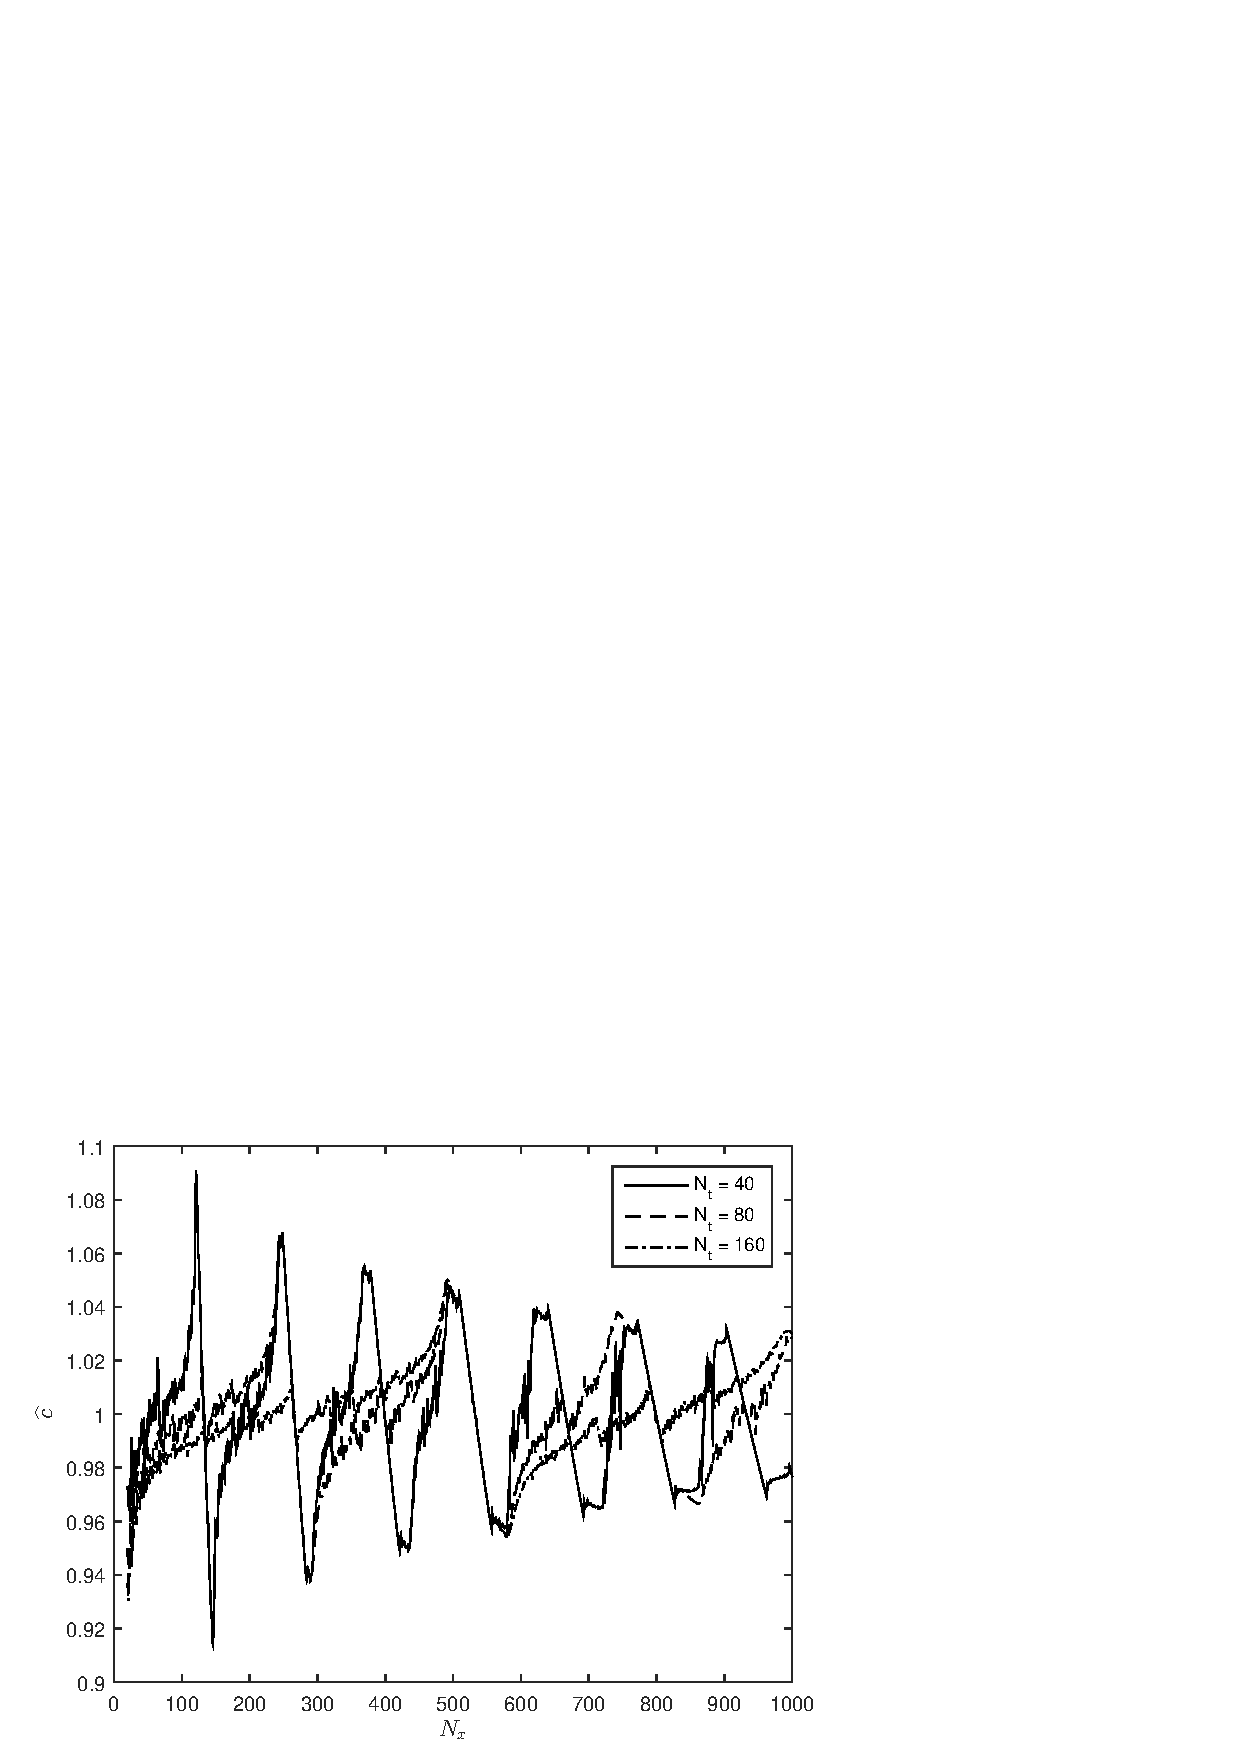
\includegraphics[width=0.9\textwidth]{barry3-k.pdf}
  \caption{ENO interpolant, followed by a flux limiter.
  \label{fig:barry3-k}}
\end{figure}
\begin{figure}[htbp]
\centering
  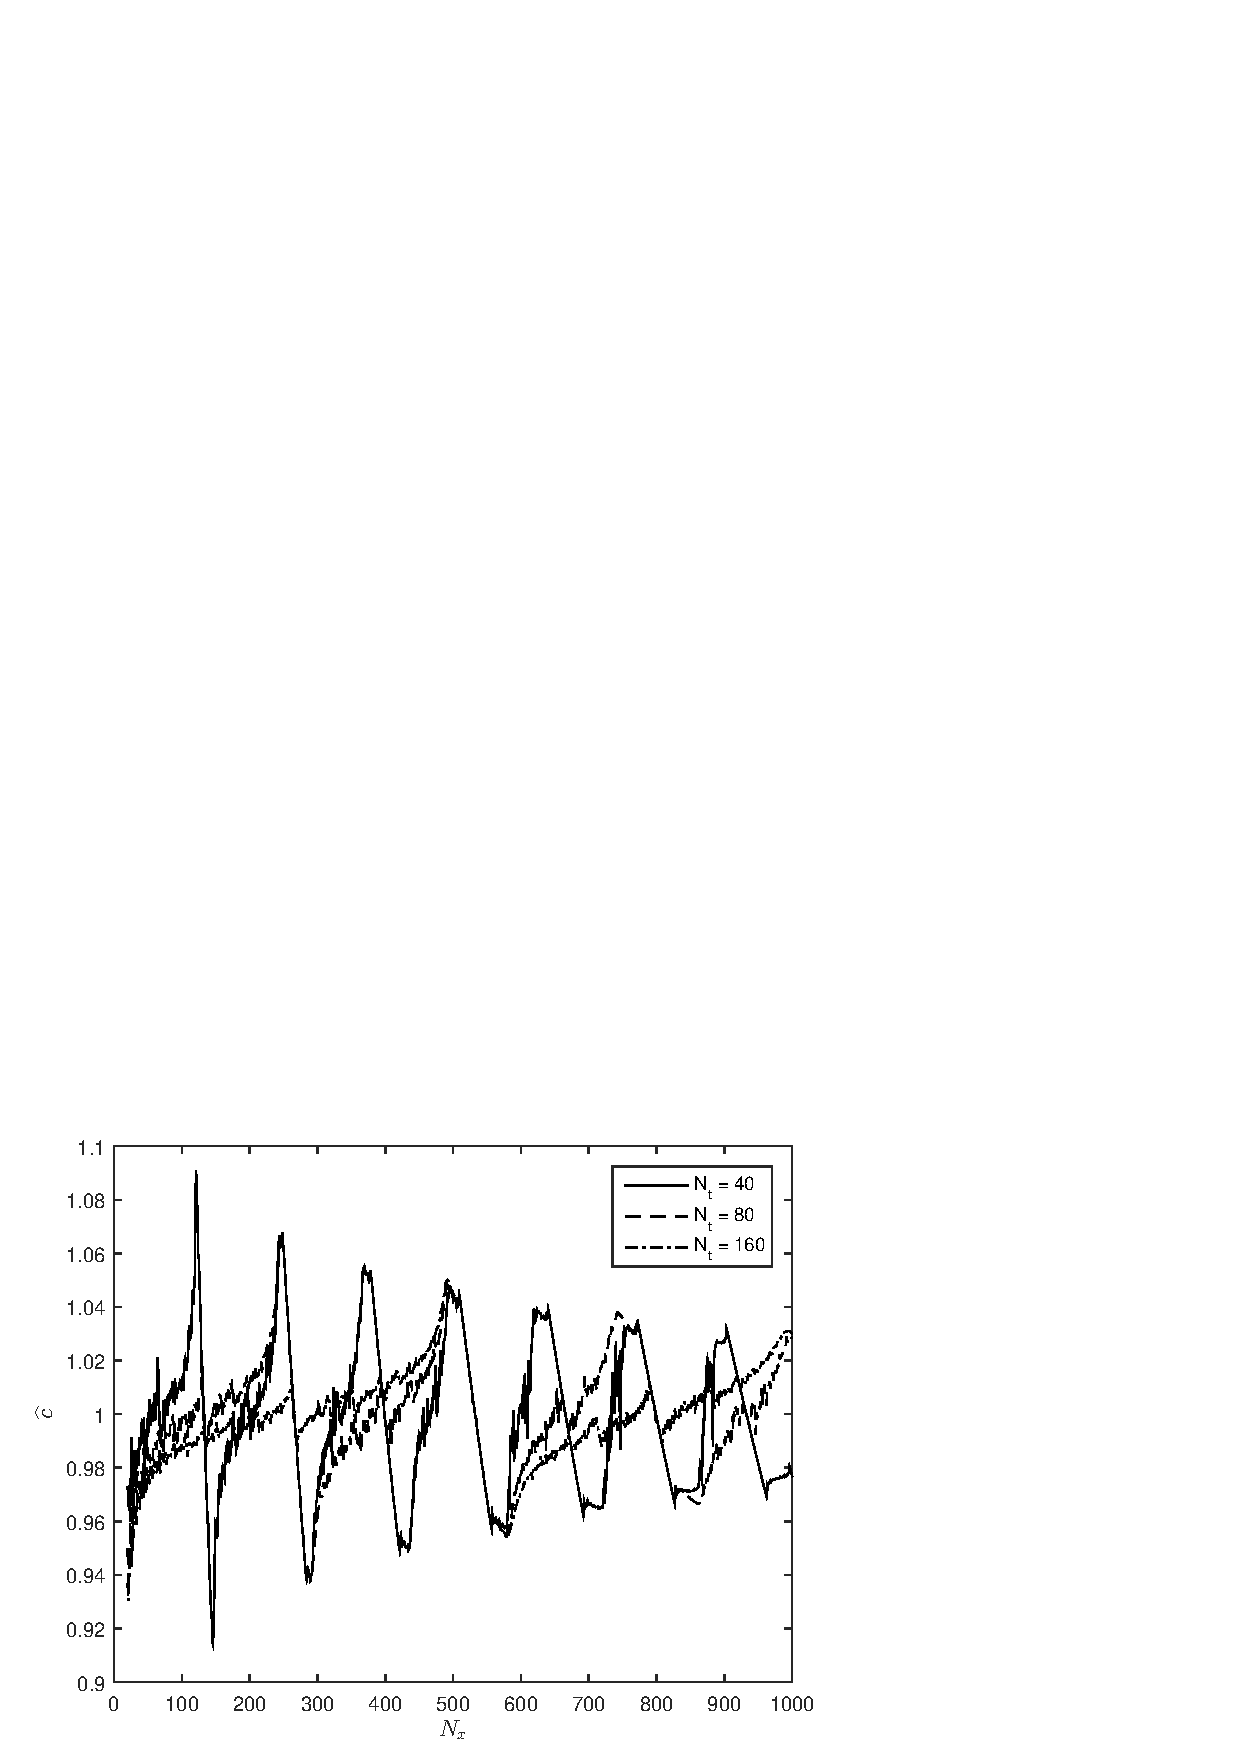
\includegraphics[width=0.9\textwidth]{barry4-k.pdf}
  \caption{ENO interpolant, no flux limiter.
  \label{fig:barry4-k}}
\end{figure}

\clearpage
\section{Numerical results for viscosity}

\begin{figure}[htbp]
\centering
  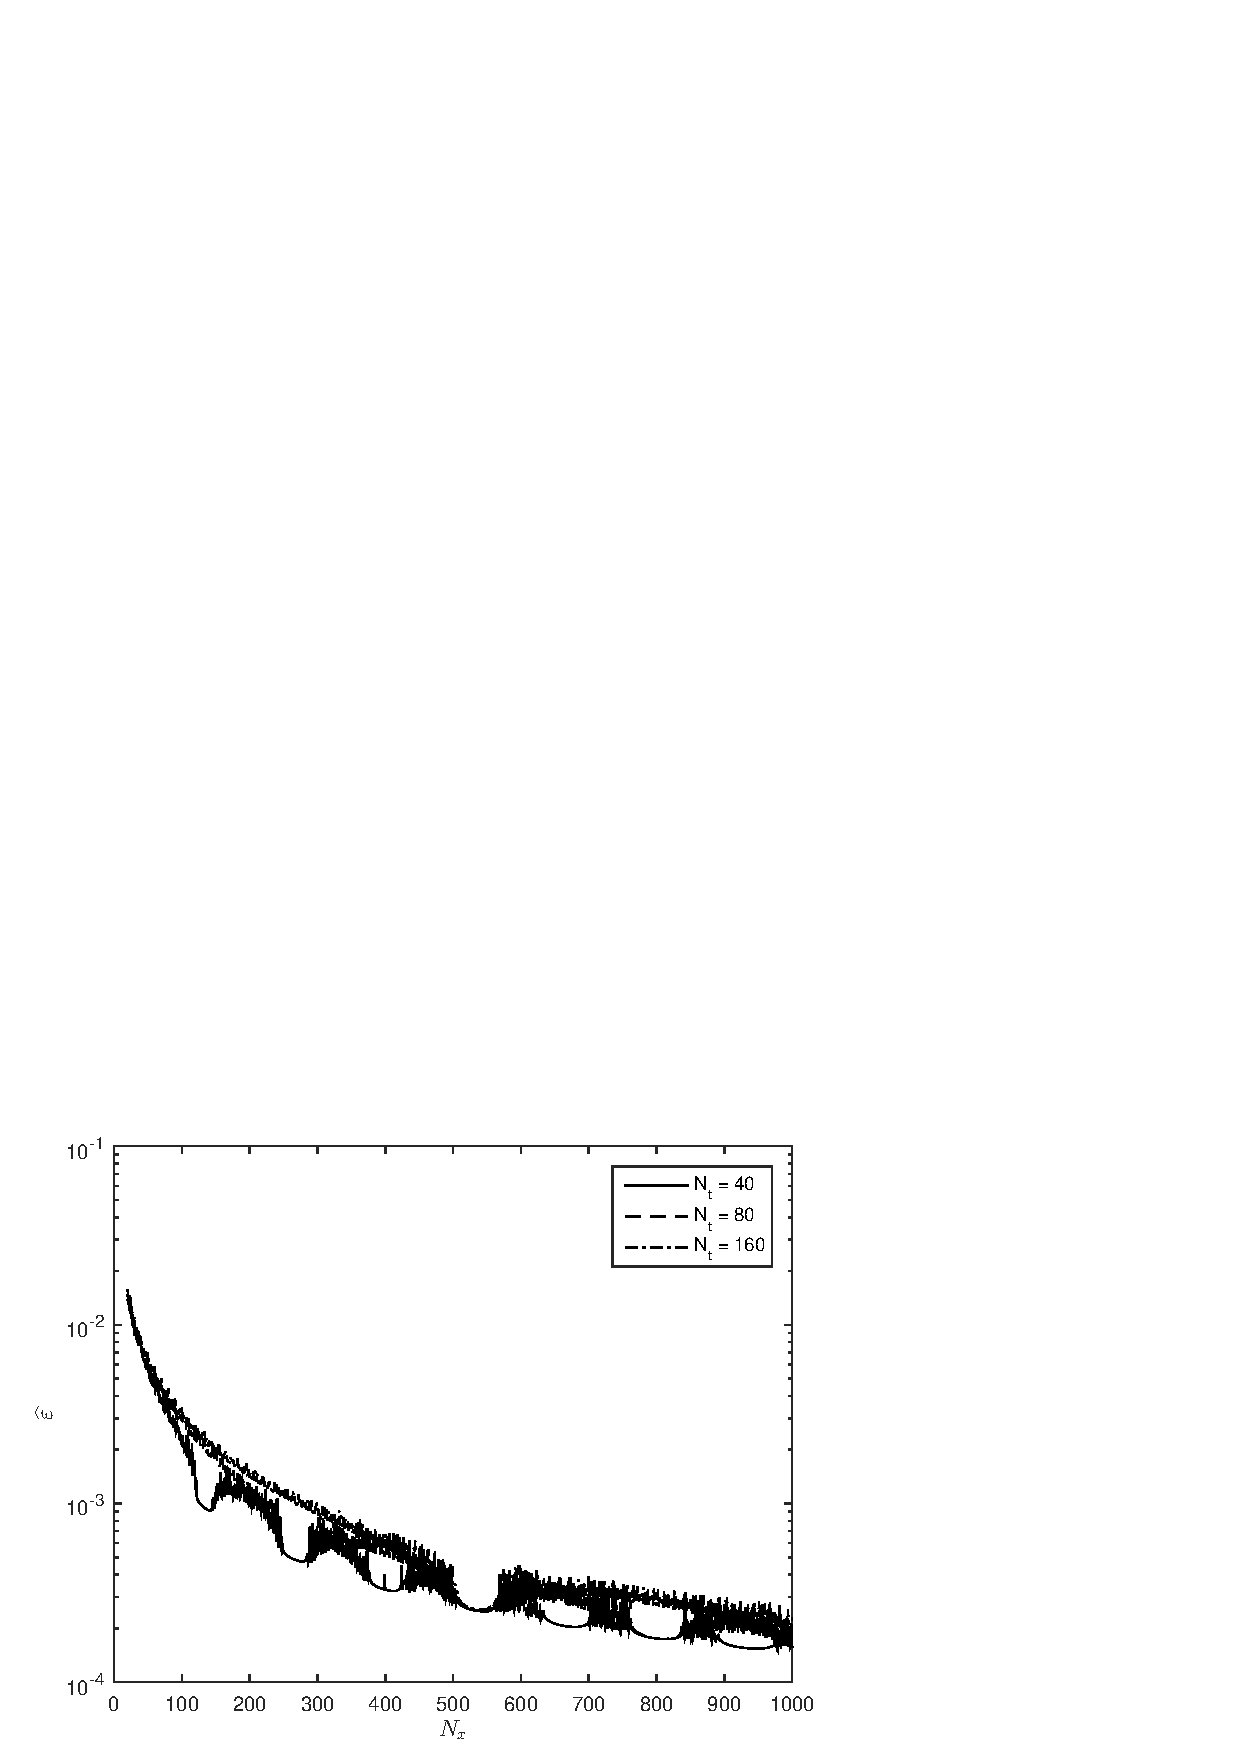
\includegraphics[width=0.9\textwidth]{barry1-eps.pdf}
  \caption{Hermite interpolant with Hyman derivative estimates and guaranteed
    monotonicity.
  \label{fig:barry1-eps}}
\end{figure}
\begin{figure}[htbp]
\centering
  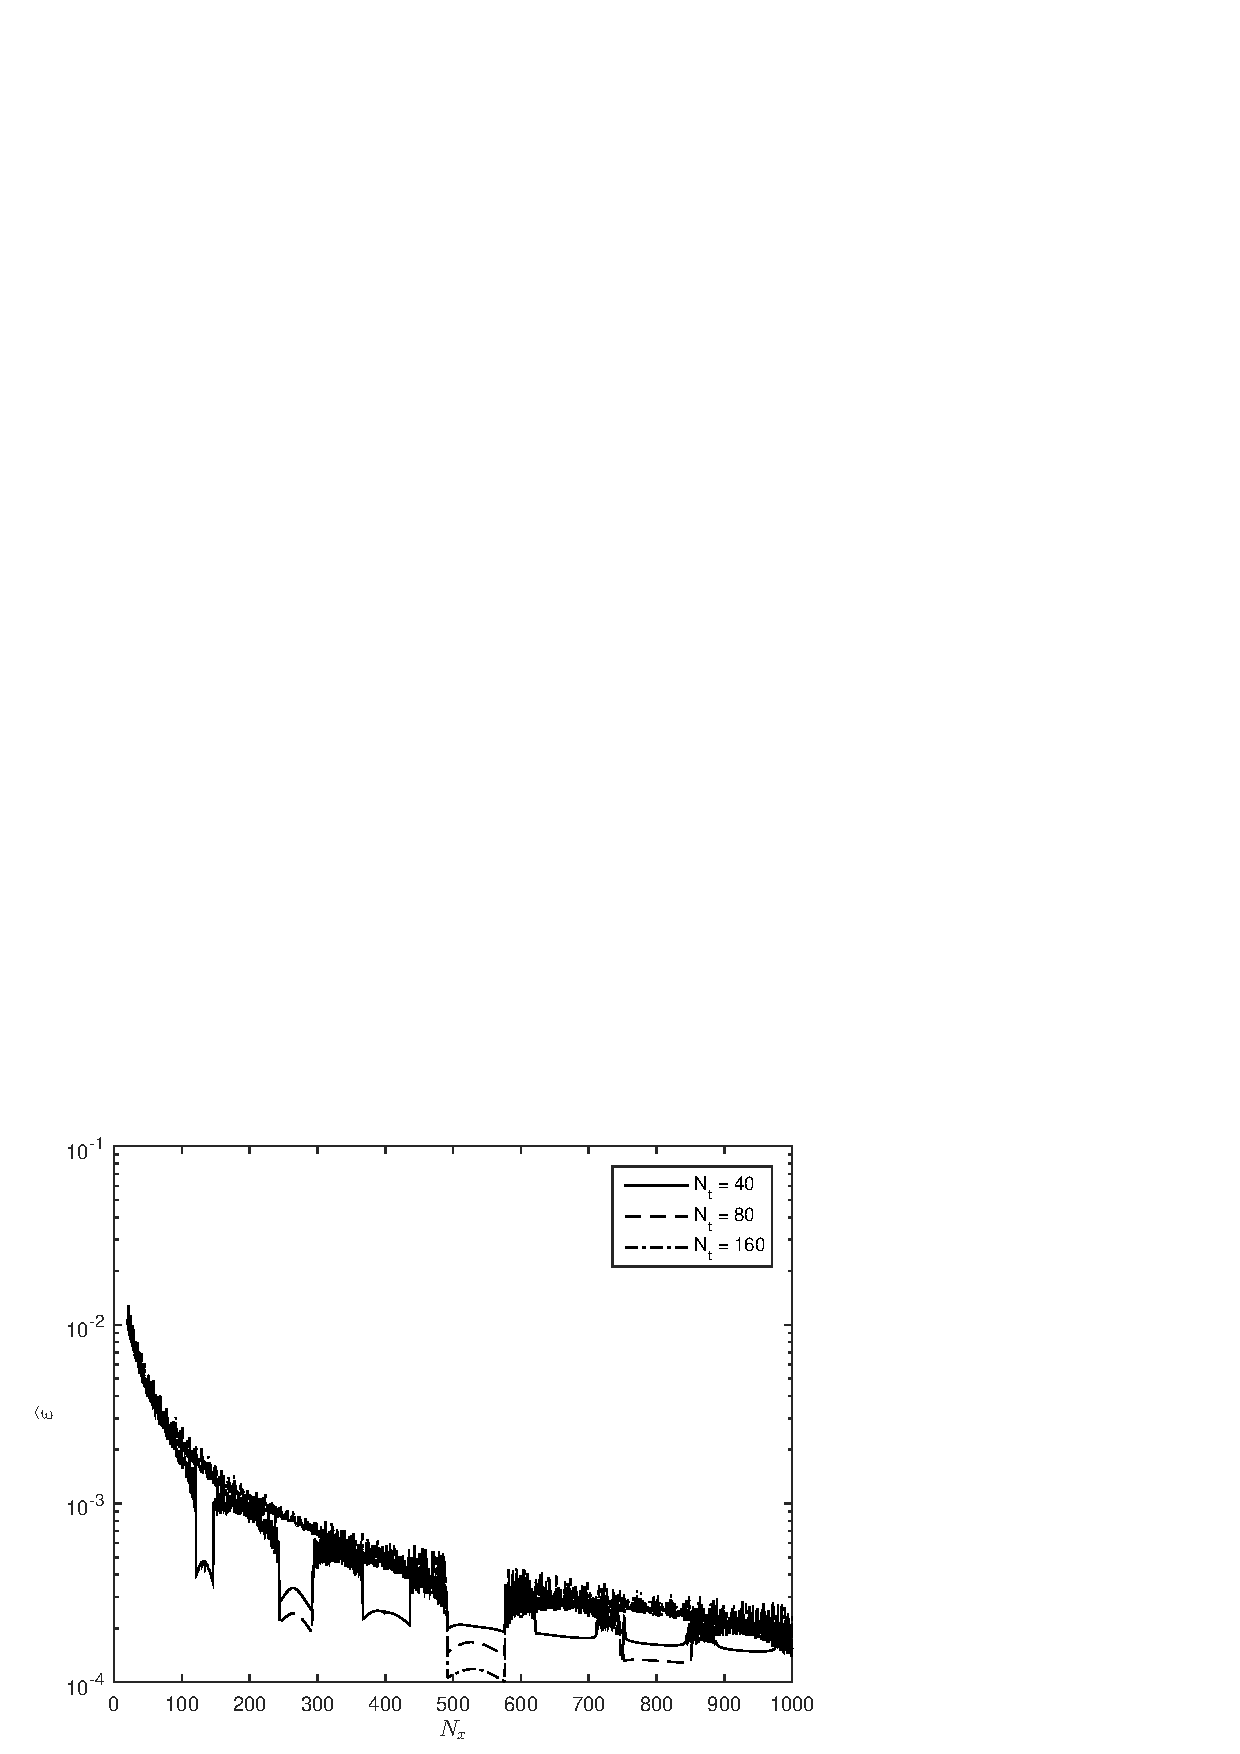
\includegraphics[width=0.9\textwidth]{barry2-eps.pdf}
  \caption{Hermite interpolant with Hyman derivative estimates.
  \label{fig:barry2-eps}}
\end{figure}
\begin{figure}[htbp]
\centering
  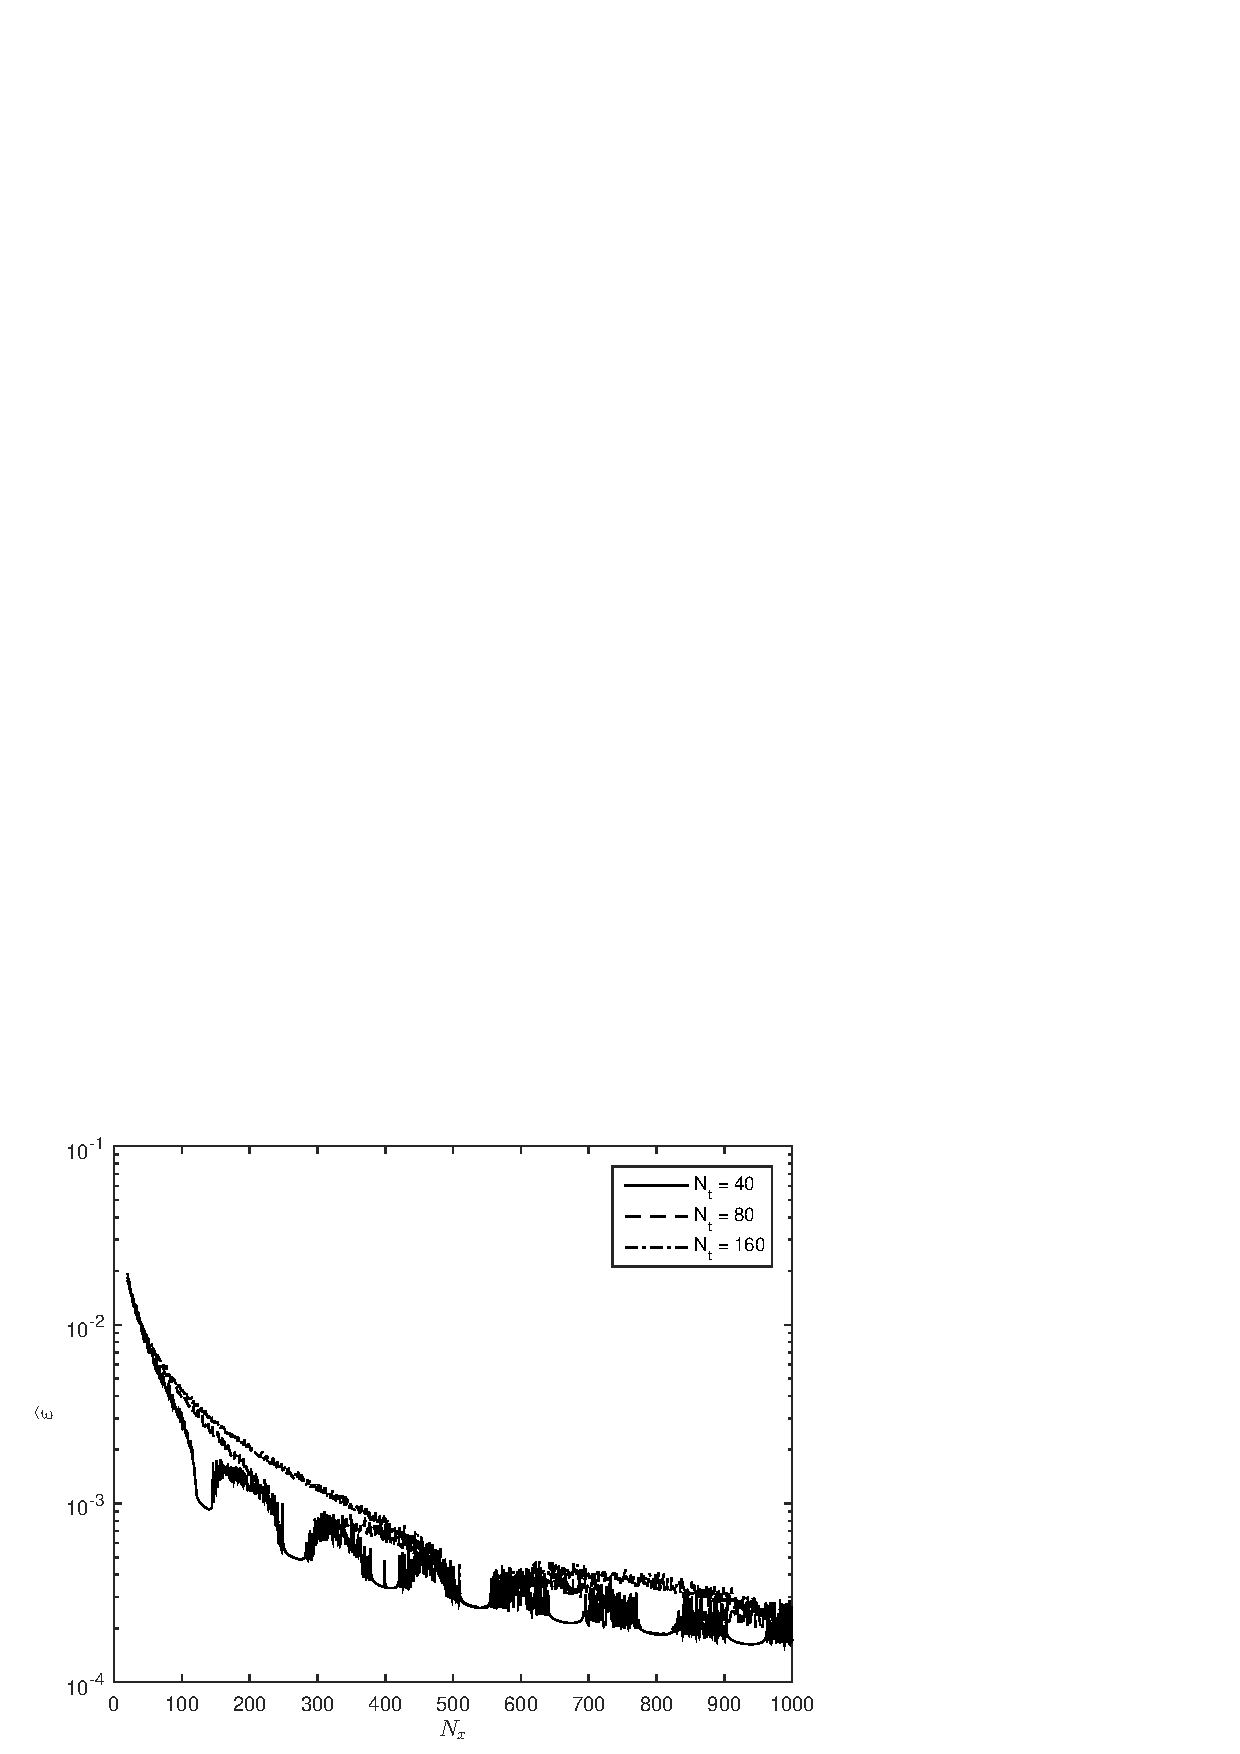
\includegraphics[width=0.9\textwidth]{barry3-eps.pdf}
  \caption{ENO interpolant, followed by a flux limiter.
  \label{fig:barry3-eps}}
\end{figure}
\begin{figure}[htbp]
\centering
  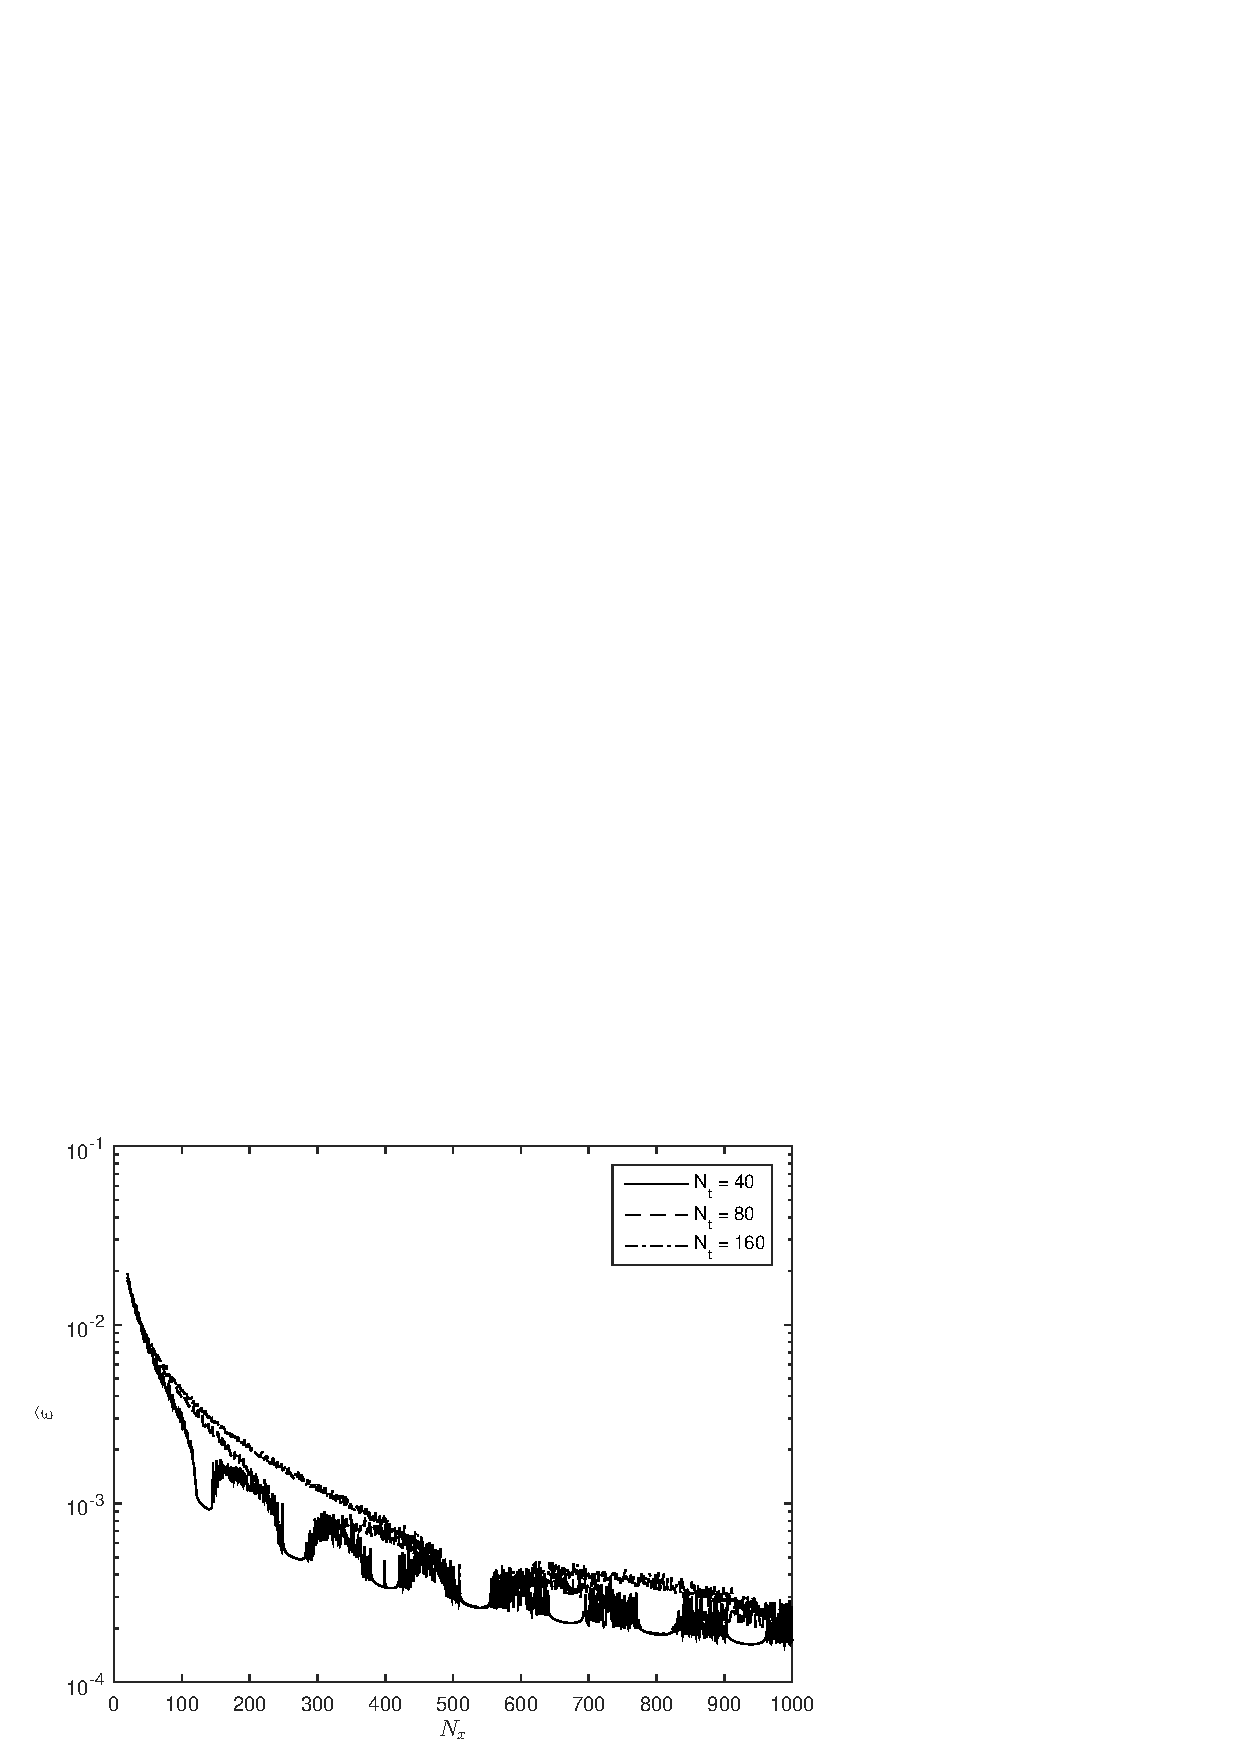
\includegraphics[width=0.9\textwidth]{barry4-eps.pdf}
  \caption{ENO interpolant, no flux limiter.
  \label{fig:barry4-eps}}
\end{figure}

\end{document}

%\end{table}

\section{Numerical results for speed}


\begin{figure}[htbp]
\centering
  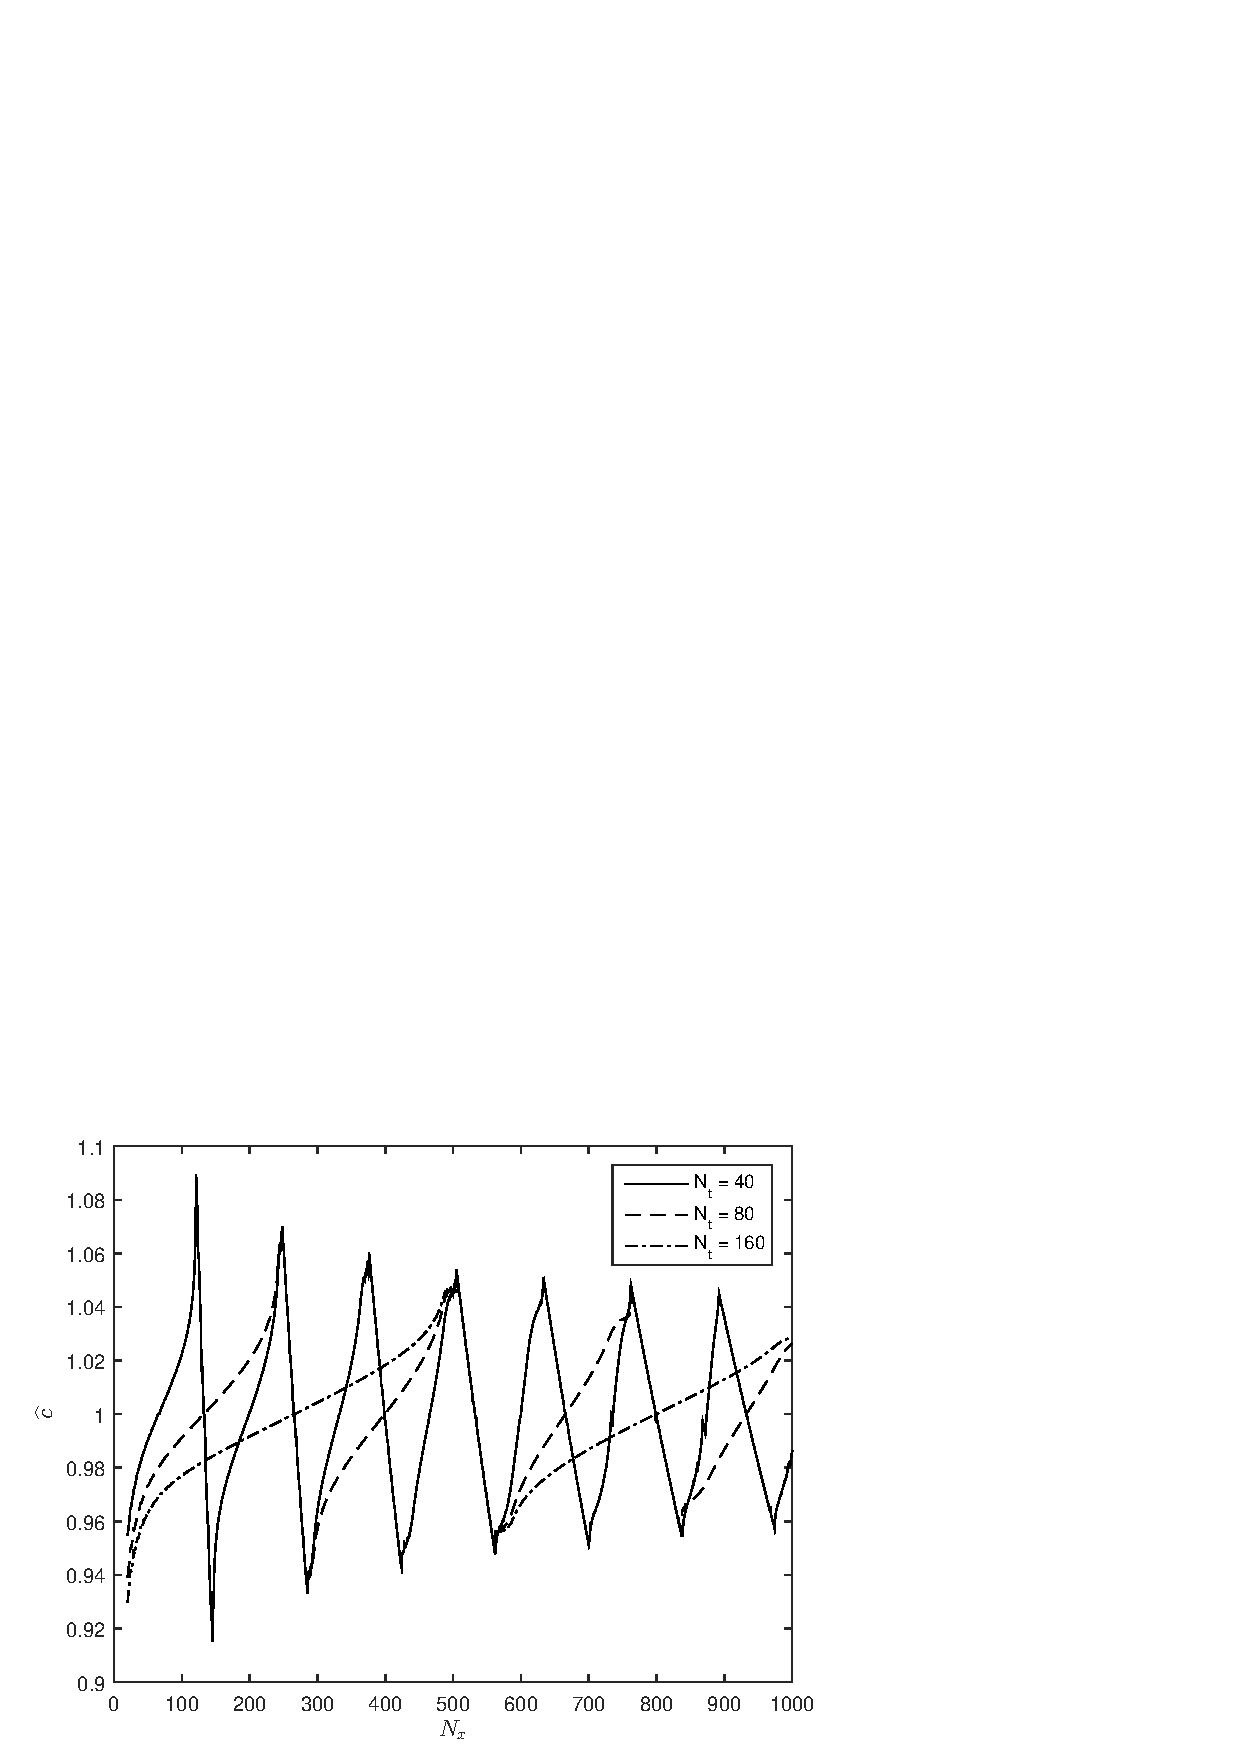
\includegraphics[width=0.9\textwidth]{barry1-k.pdf}
  \caption{Hermite interpolant with Hyman derivative estimates and guaranteed
    monotonicity.
  \label{fig:barry1-k}}
\end{figure}
\begin{figure}[htbp]
\centering
  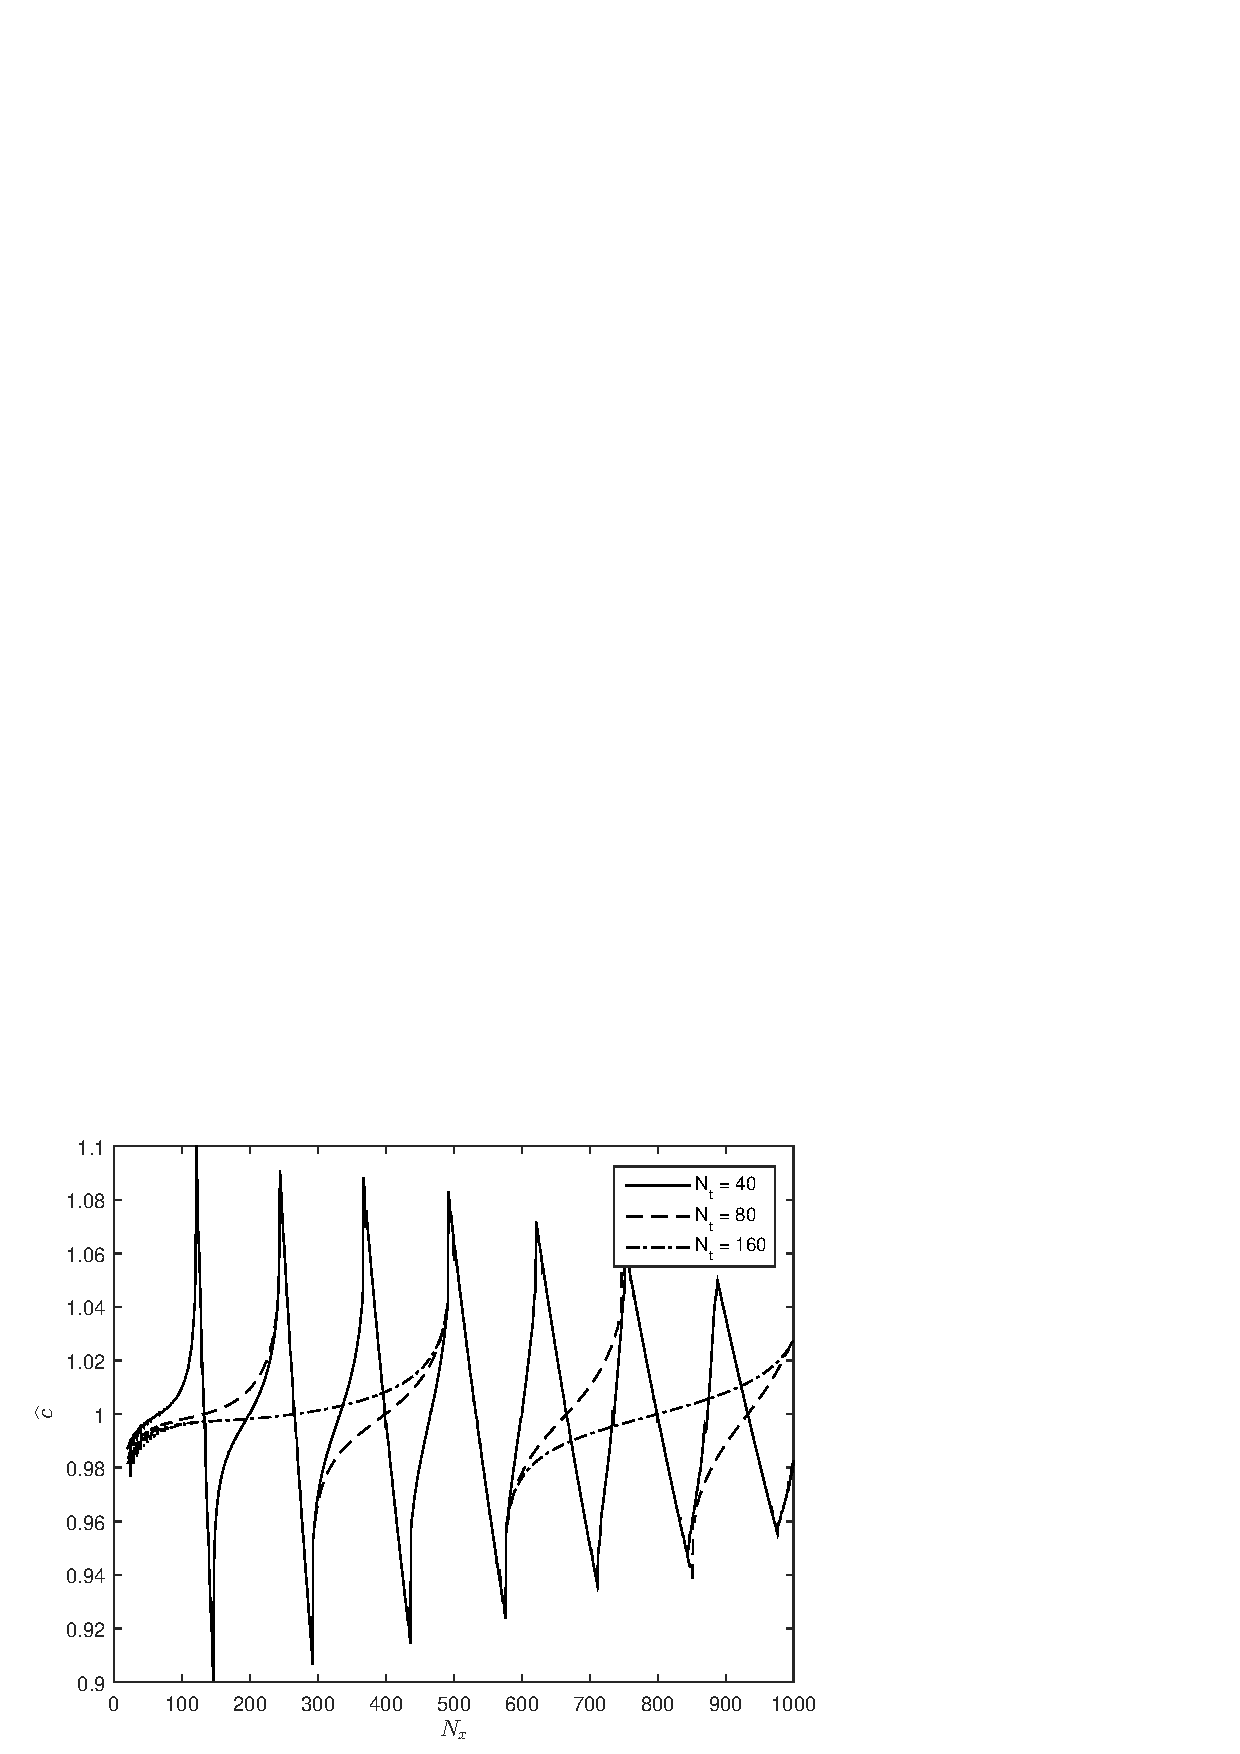
\includegraphics[width=0.9\textwidth]{barry2-k.pdf}
  \caption{Hermite interpolant with Hyman derivative estimates.
  \label{fig:barry2-k}}
\end{figure}
\begin{figure}[htbp]
\centering
  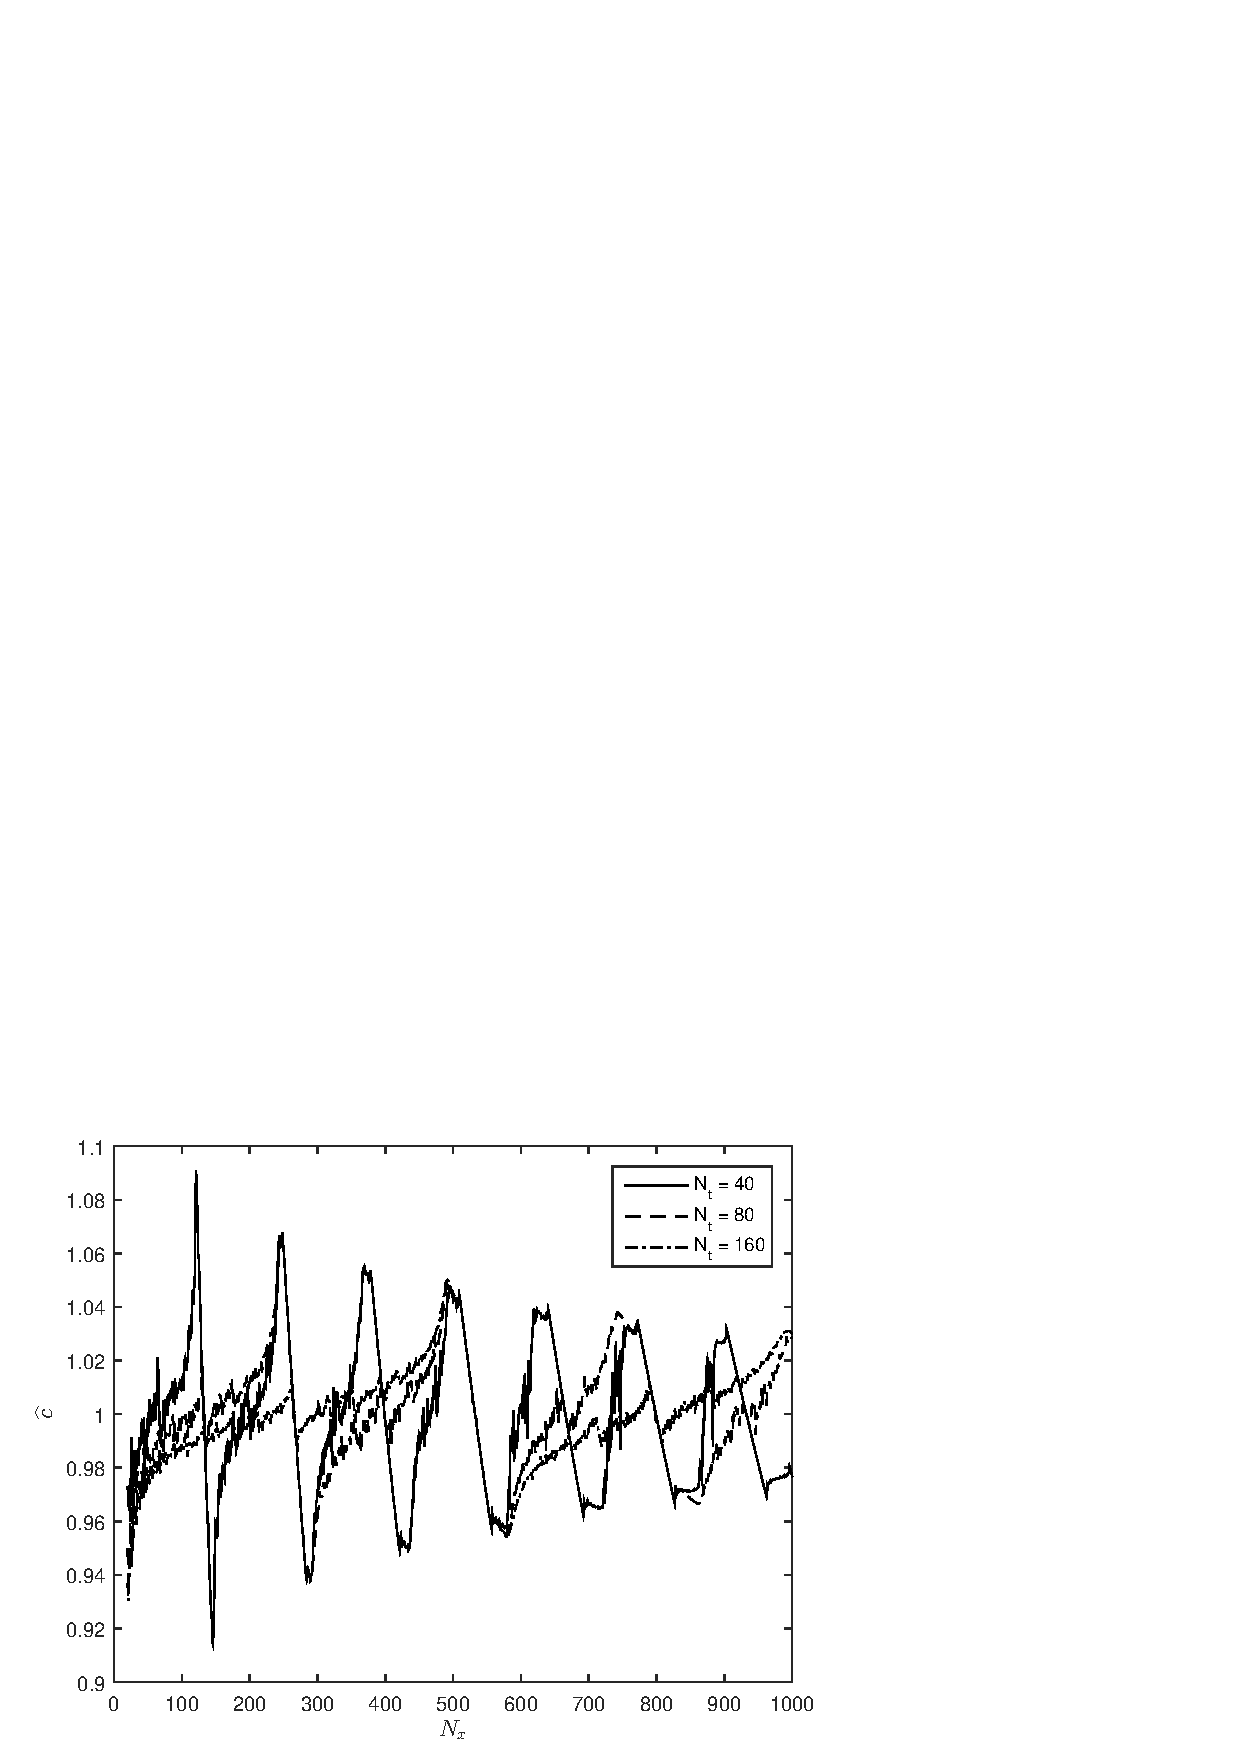
\includegraphics[width=0.9\textwidth]{barry3-k.pdf}
  \caption{ENO interpolant, followed by a flux limiter.
  \label{fig:barry3-k}}
\end{figure}
\begin{figure}[htbp]
\centering
  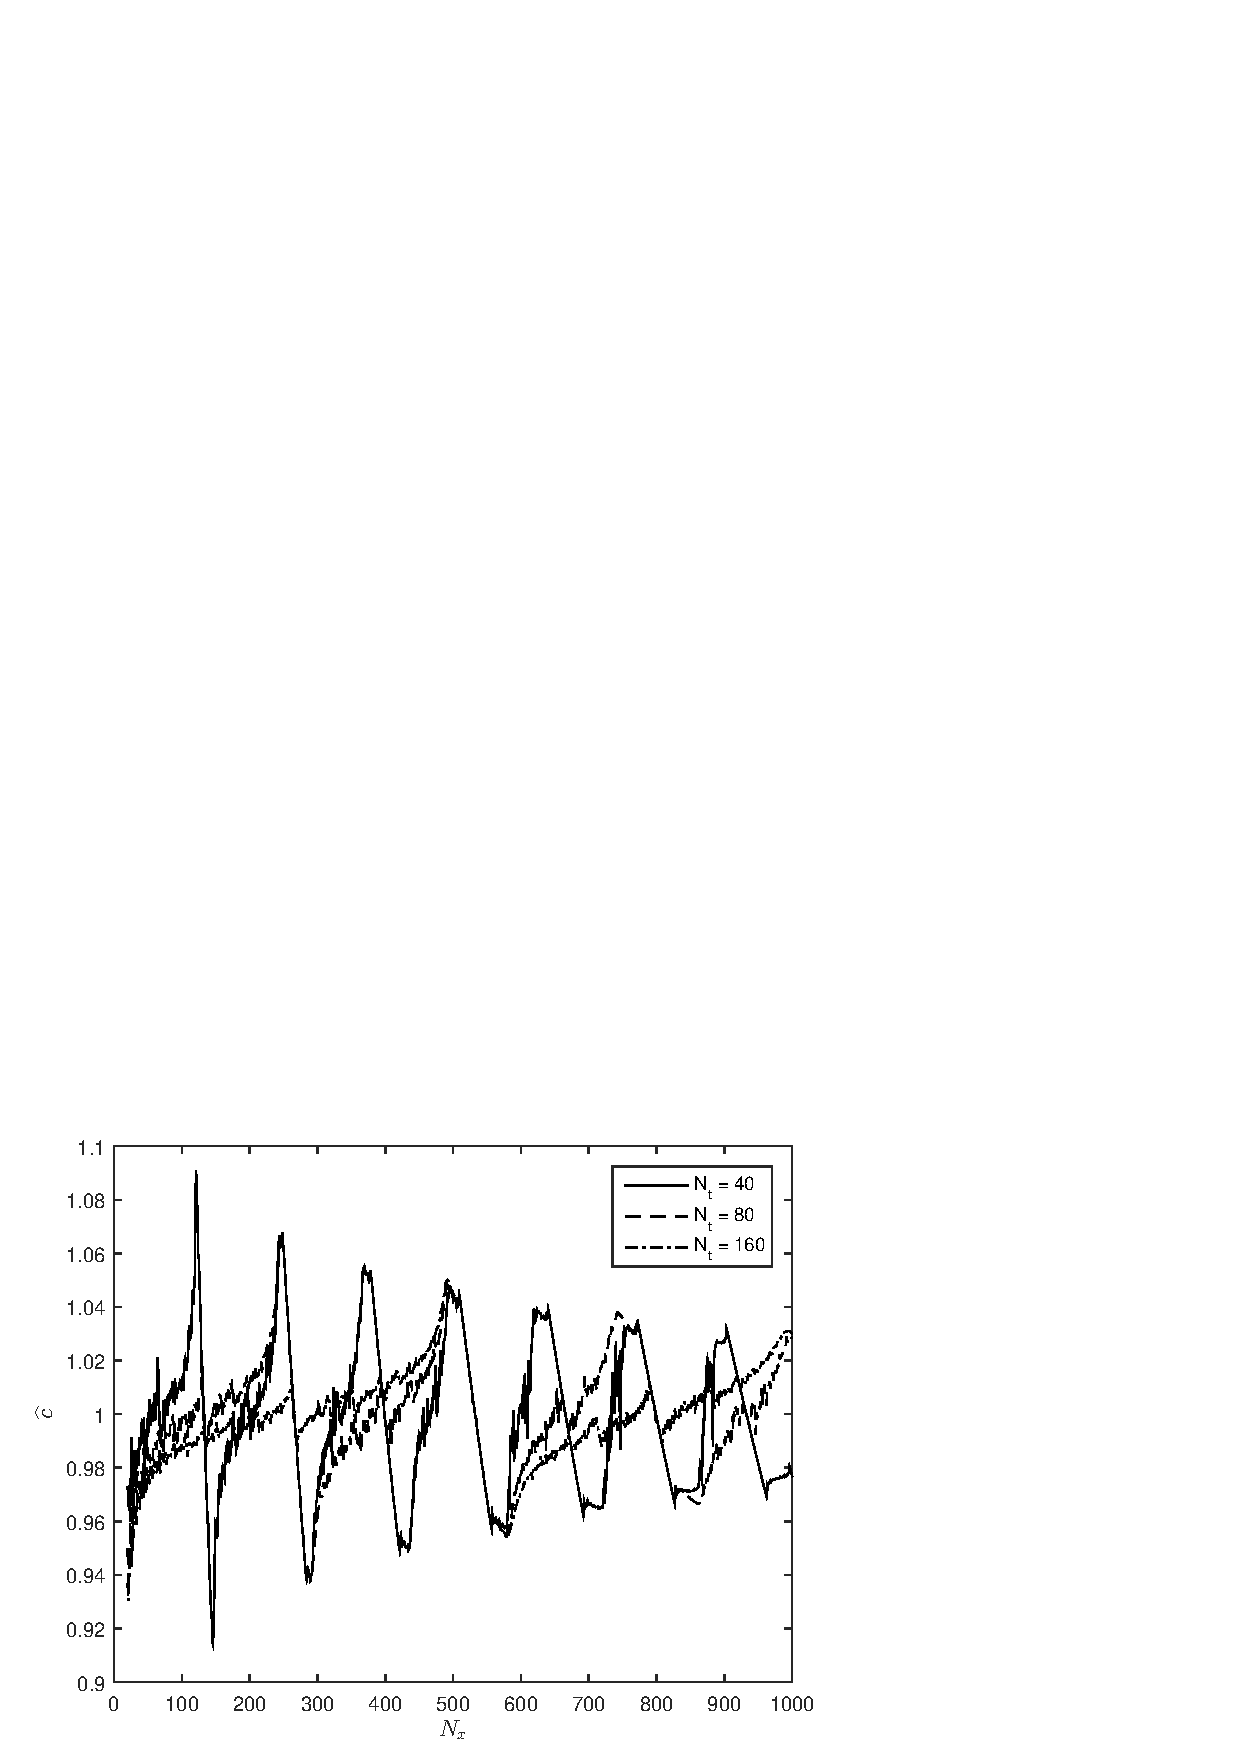
\includegraphics[width=0.9\textwidth]{barry4-k.pdf}
  \caption{ENO interpolant, no flux limiter.
  \label{fig:barry4-k}}
\end{figure}

\clearpage
\section{Numerical results for viscosity}

\begin{figure}[htbp]
\centering
  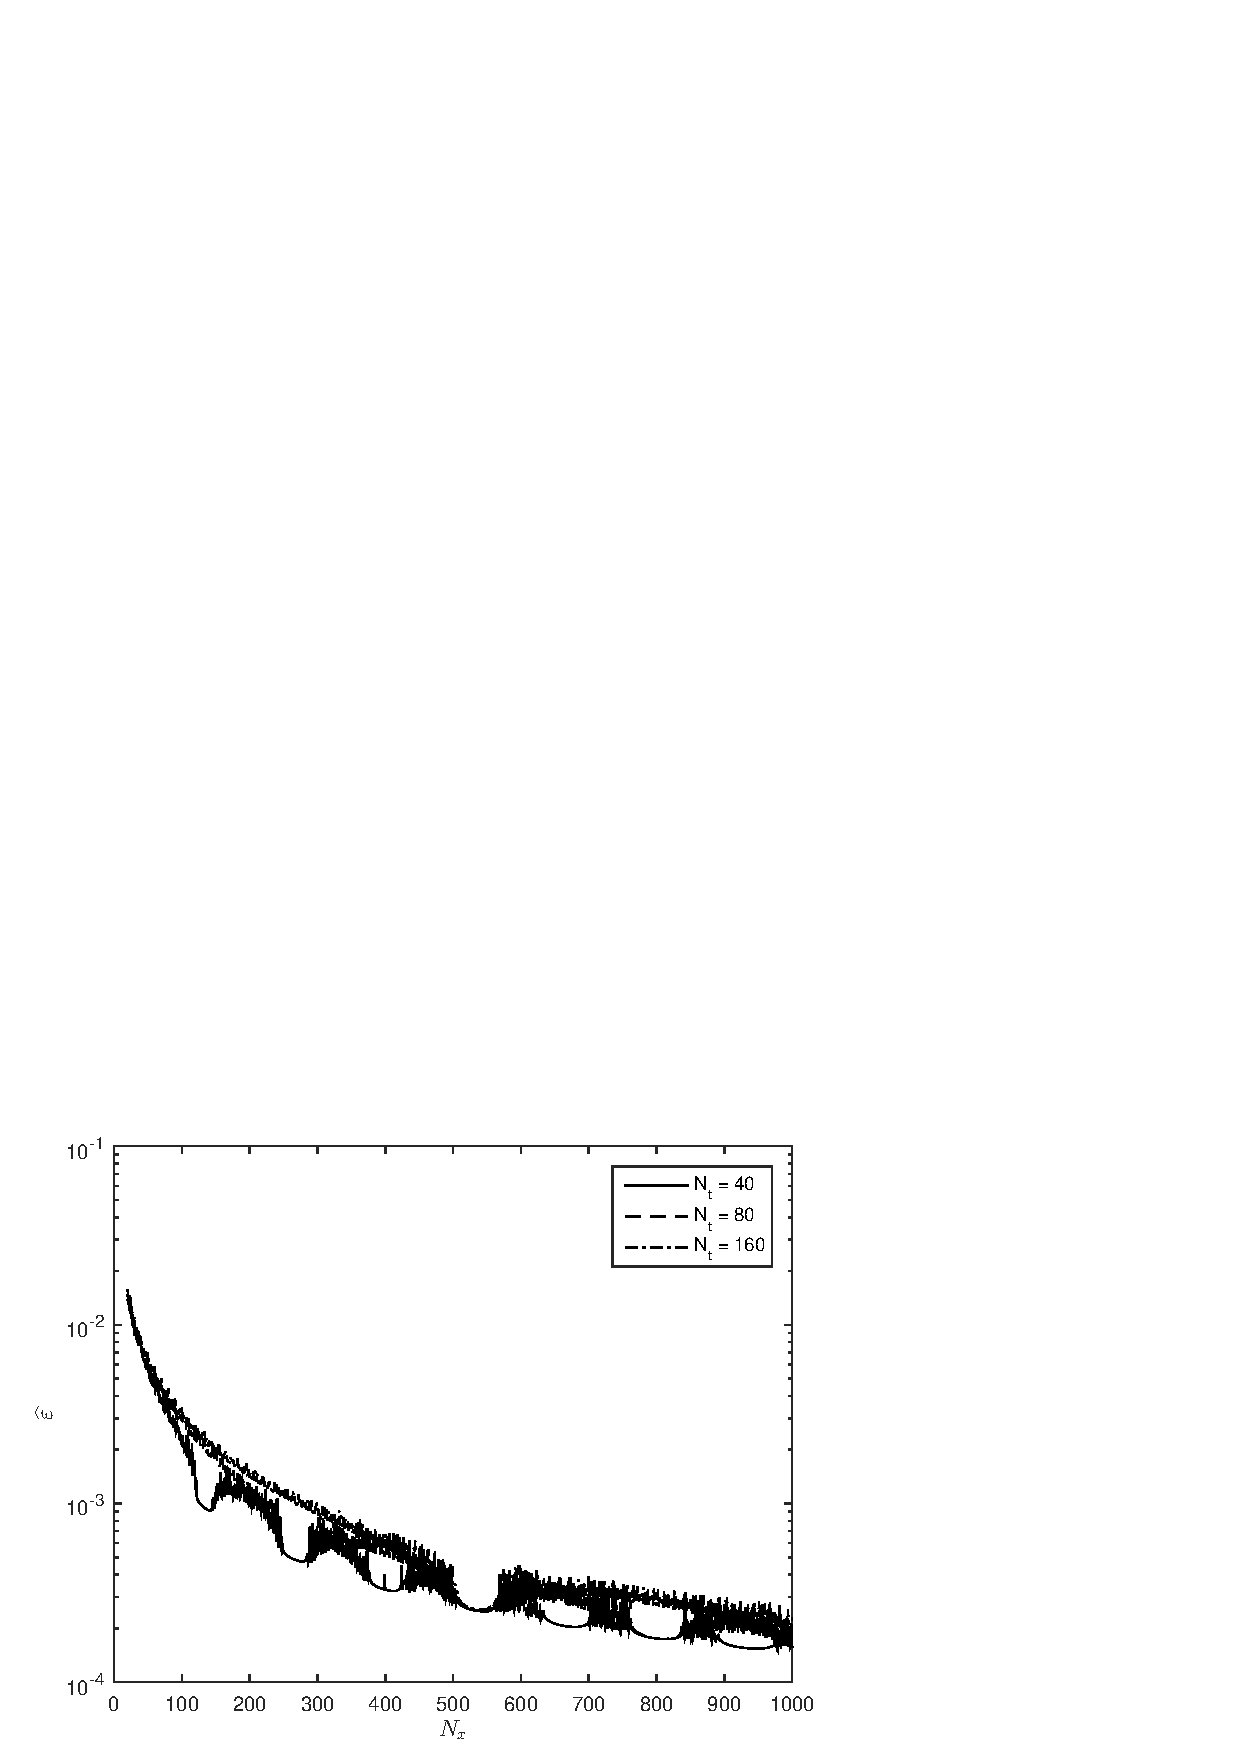
\includegraphics[width=0.9\textwidth]{barry1-eps.pdf}
  \caption{Hermite interpolant with Hyman derivative estimates and guaranteed
    monotonicity.
  \label{fig:barry1-eps}}
\end{figure}
\begin{figure}[htbp]
\centering
  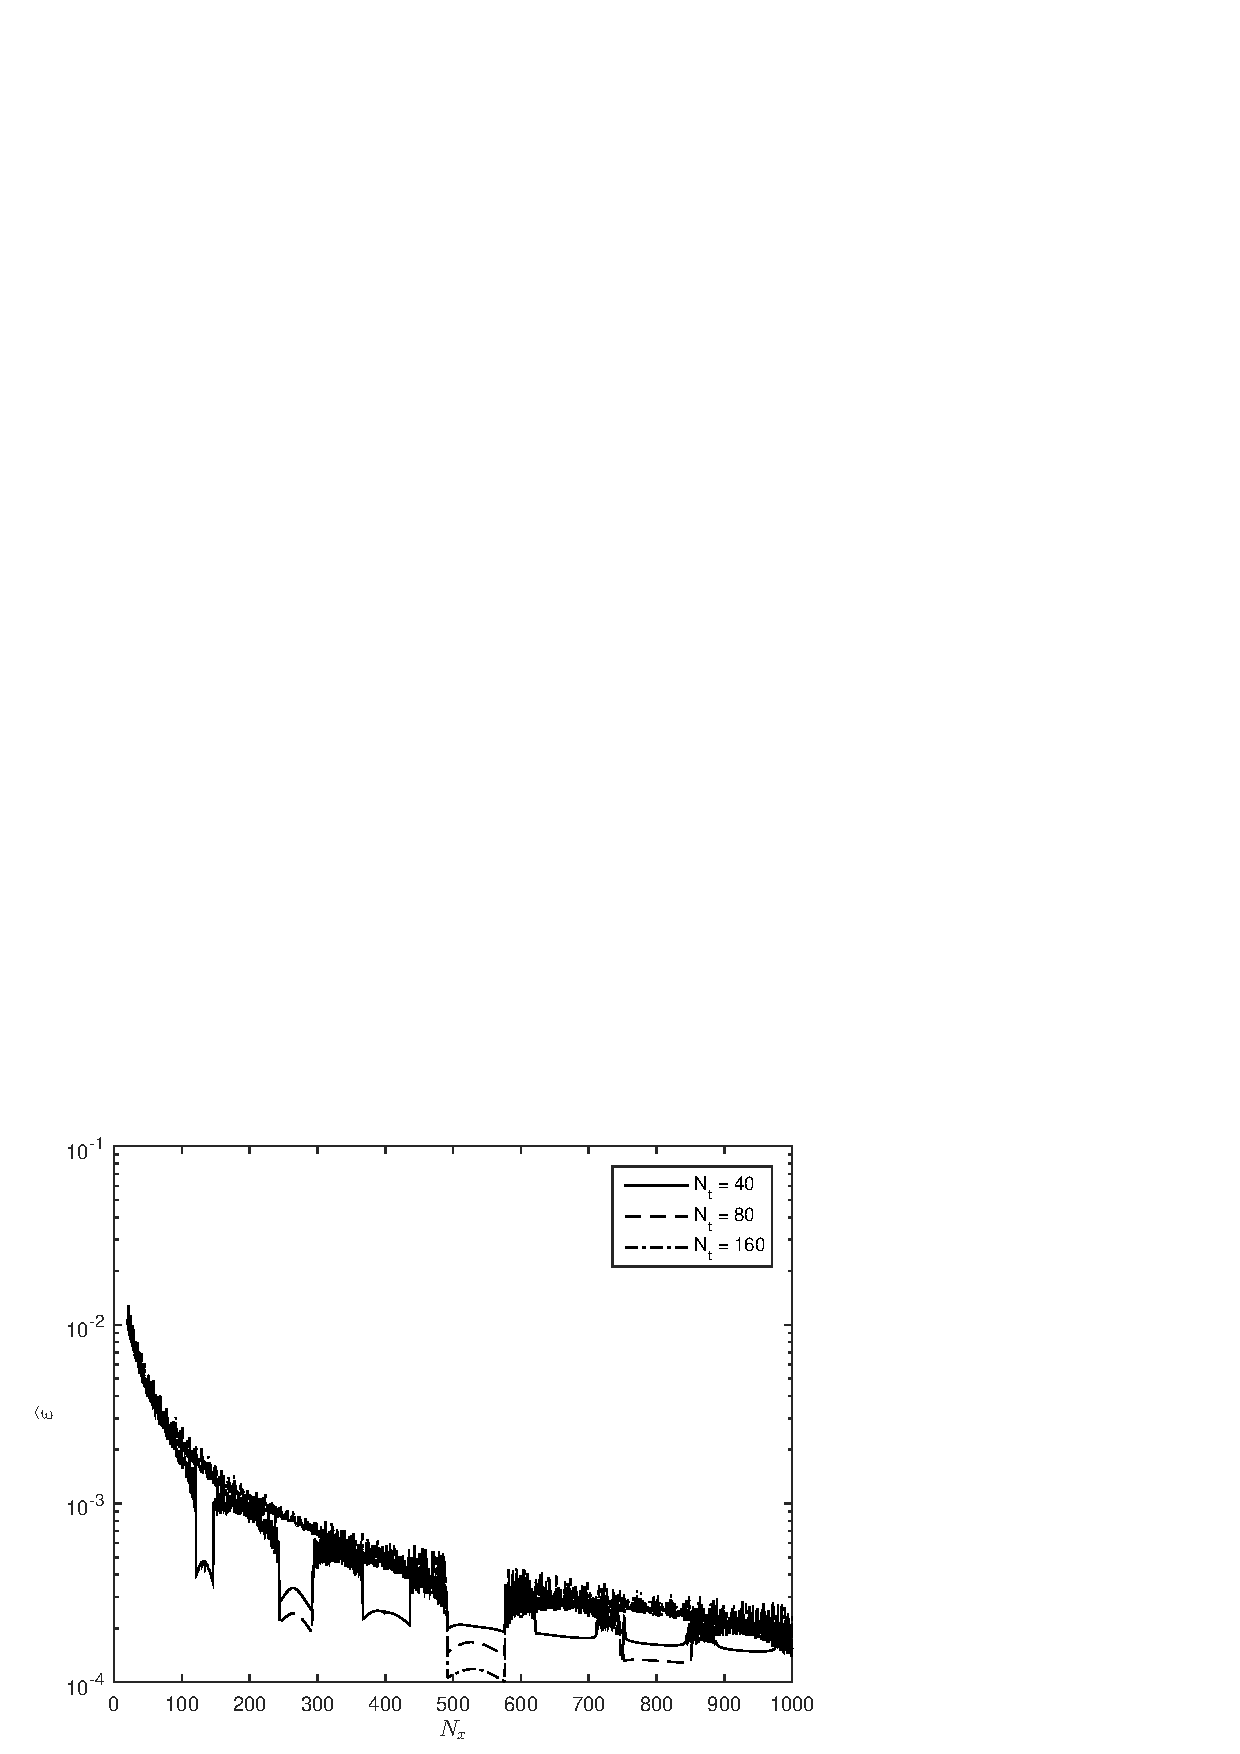
\includegraphics[width=0.9\textwidth]{barry2-eps.pdf}
  \caption{Hermite interpolant with Hyman derivative estimates.
  \label{fig:barry2-eps}}
\end{figure}
\begin{figure}[htbp]
\centering
  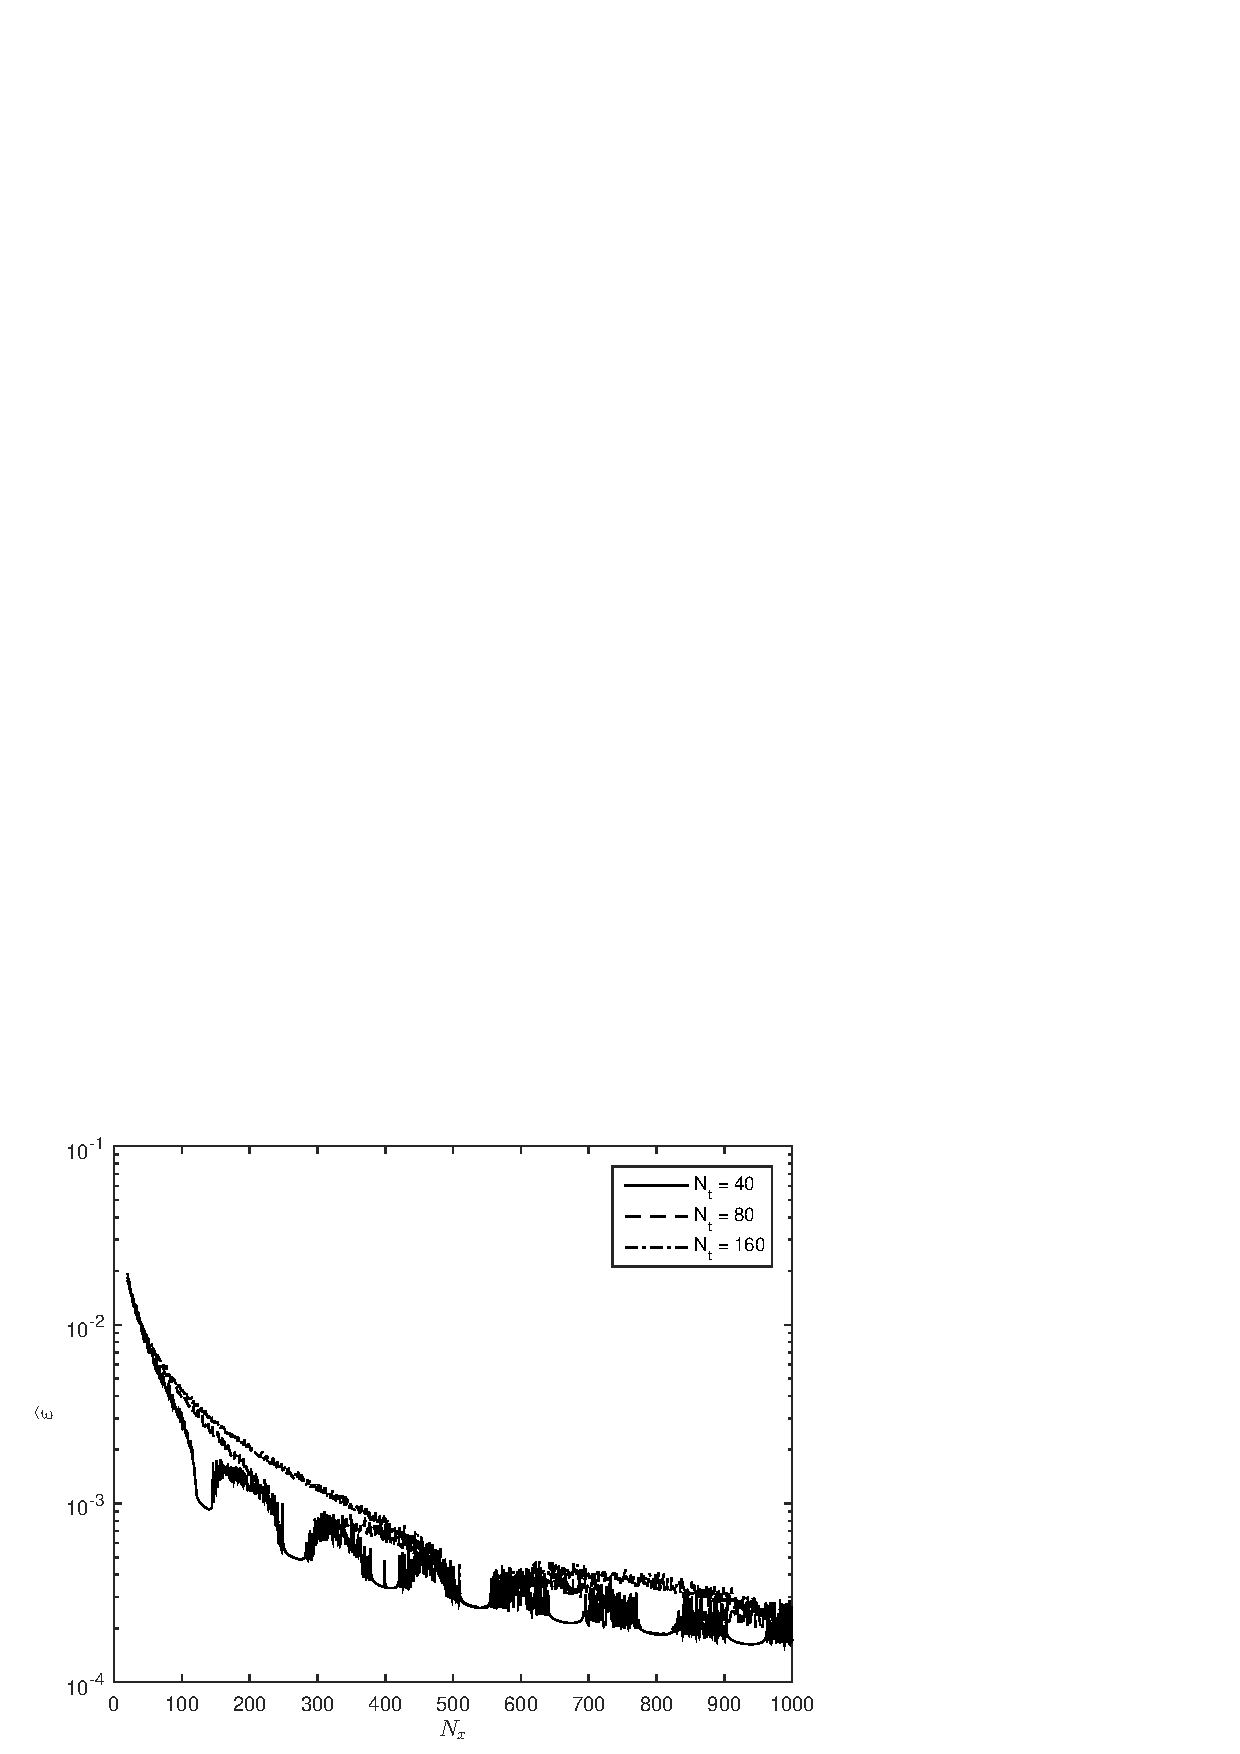
\includegraphics[width=0.9\textwidth]{barry3-eps.pdf}
  \caption{ENO interpolant, followed by a flux limiter.
  \label{fig:barry3-eps}}
\end{figure}
\begin{figure}[htbp]
\centering
  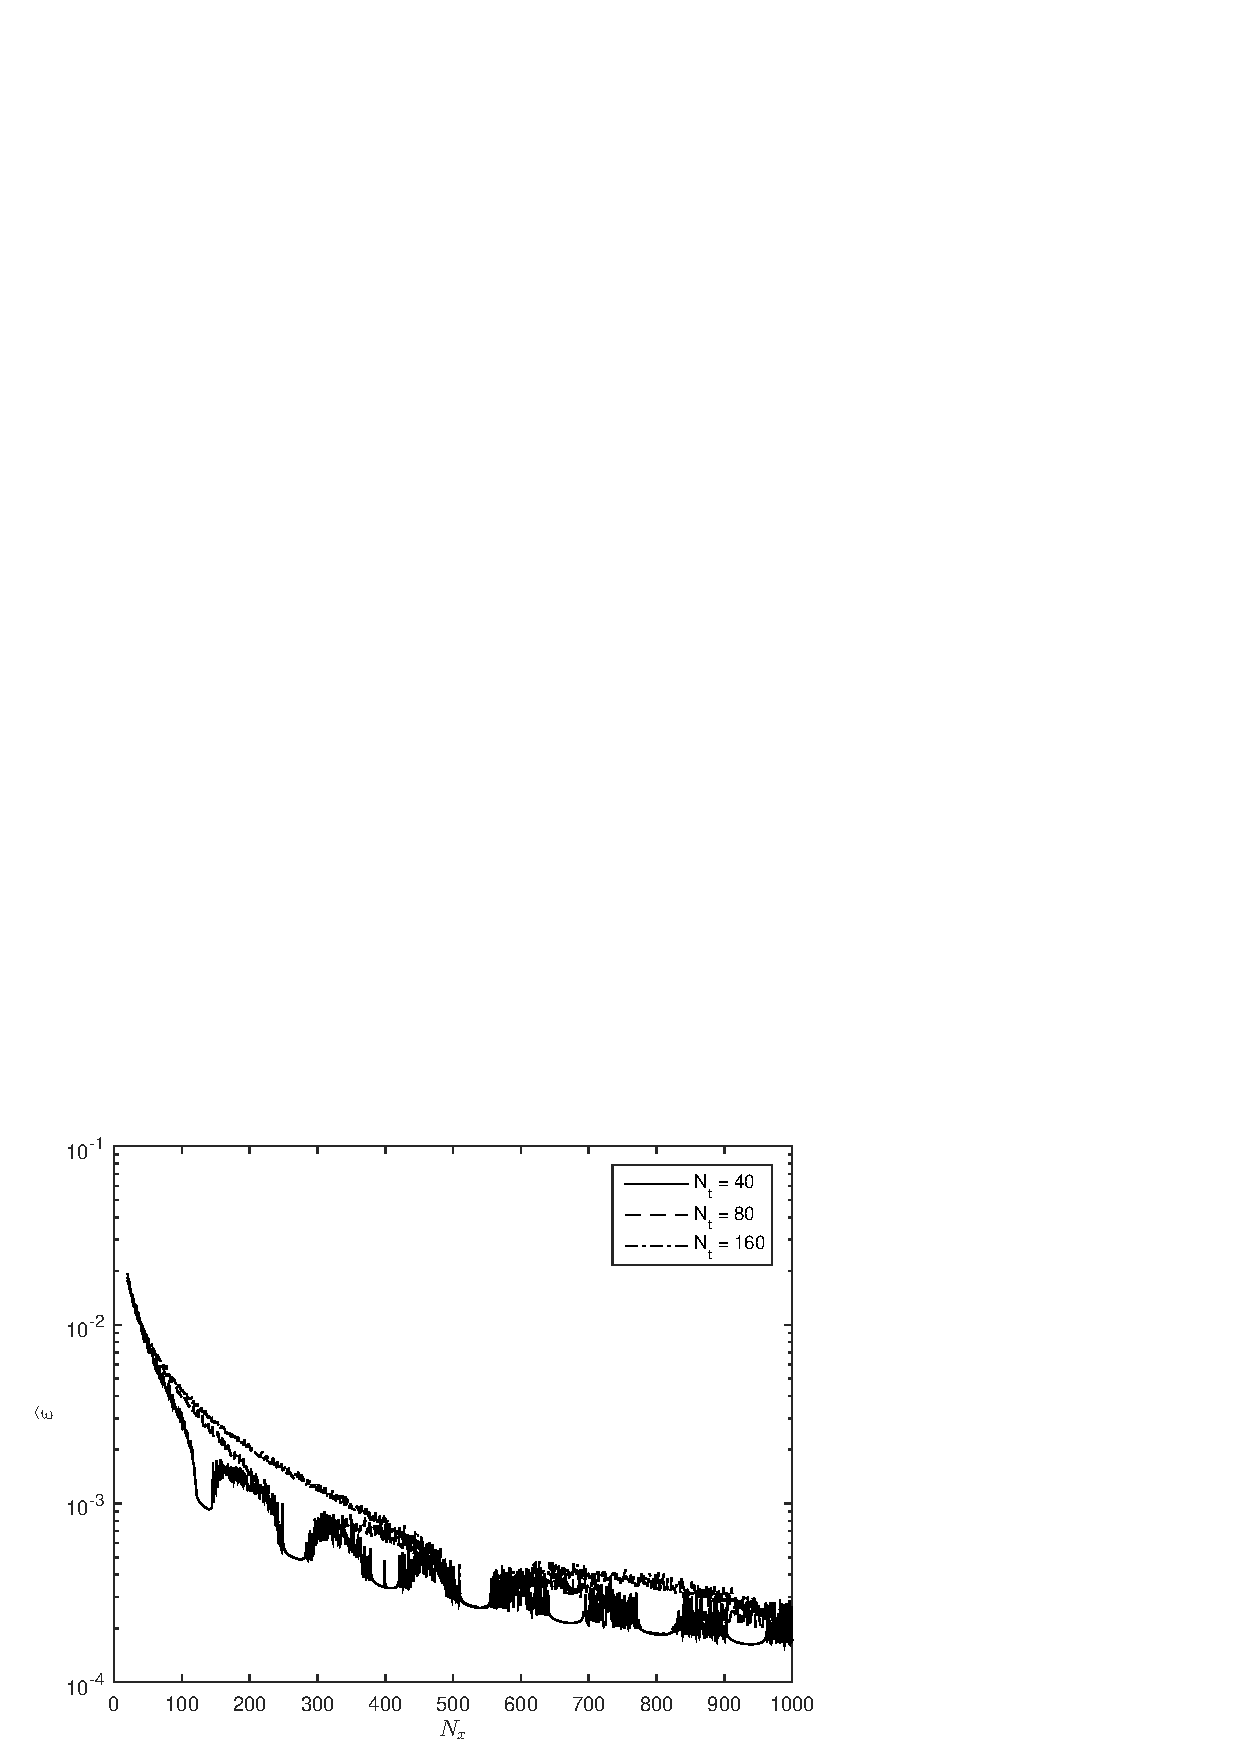
\includegraphics[width=0.9\textwidth]{barry4-eps.pdf}
  \caption{ENO interpolant, no flux limiter.
  \label{fig:barry4-eps}}
\end{figure}

\end{document}

%\end{table}

\section{Numerical results for speed}


\begin{figure}[htbp]
\centering
  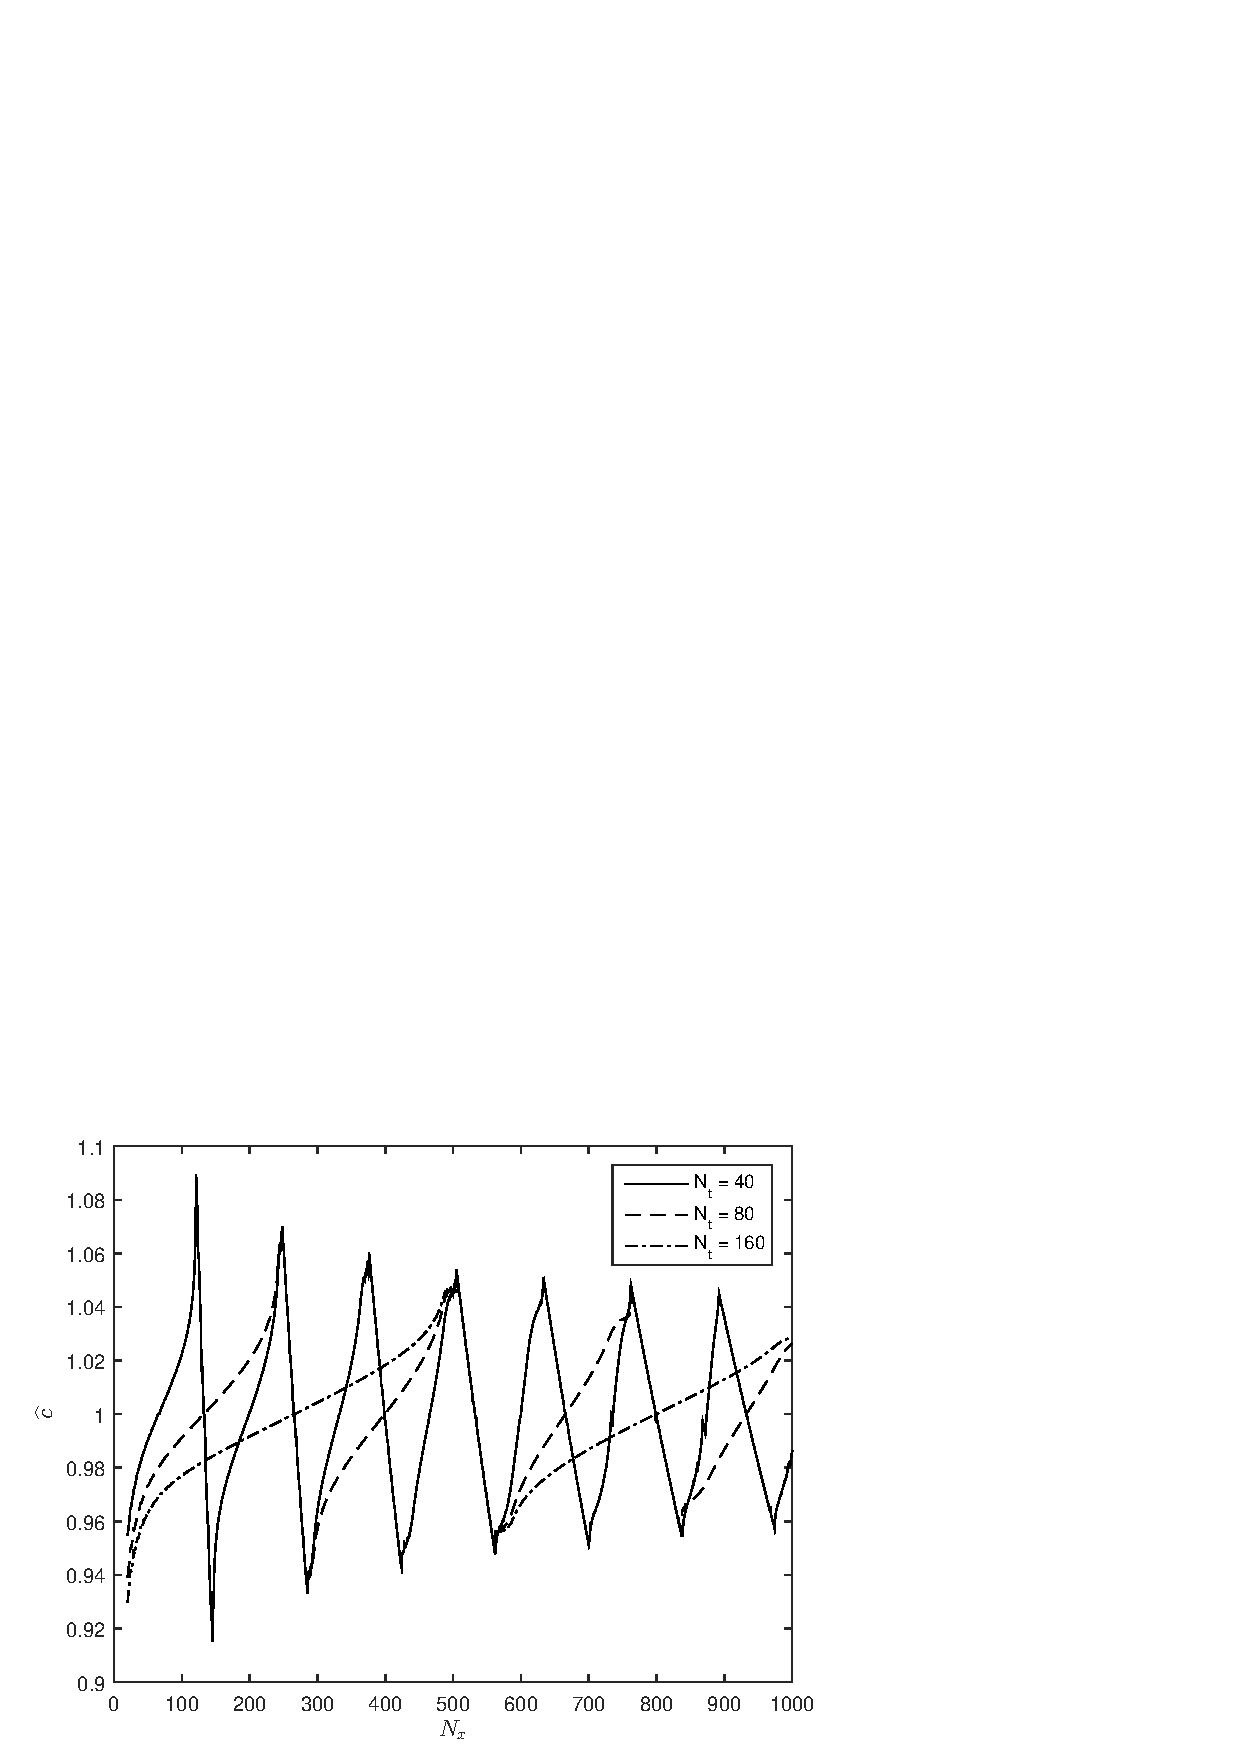
\includegraphics[width=0.9\textwidth]{barry1-k.pdf}
  \caption{Hermite interpolant with Hyman derivative estimates and guaranteed
    monotonicity.
  \label{fig:barry1-k}}
\end{figure}
\begin{figure}[htbp]
\centering
  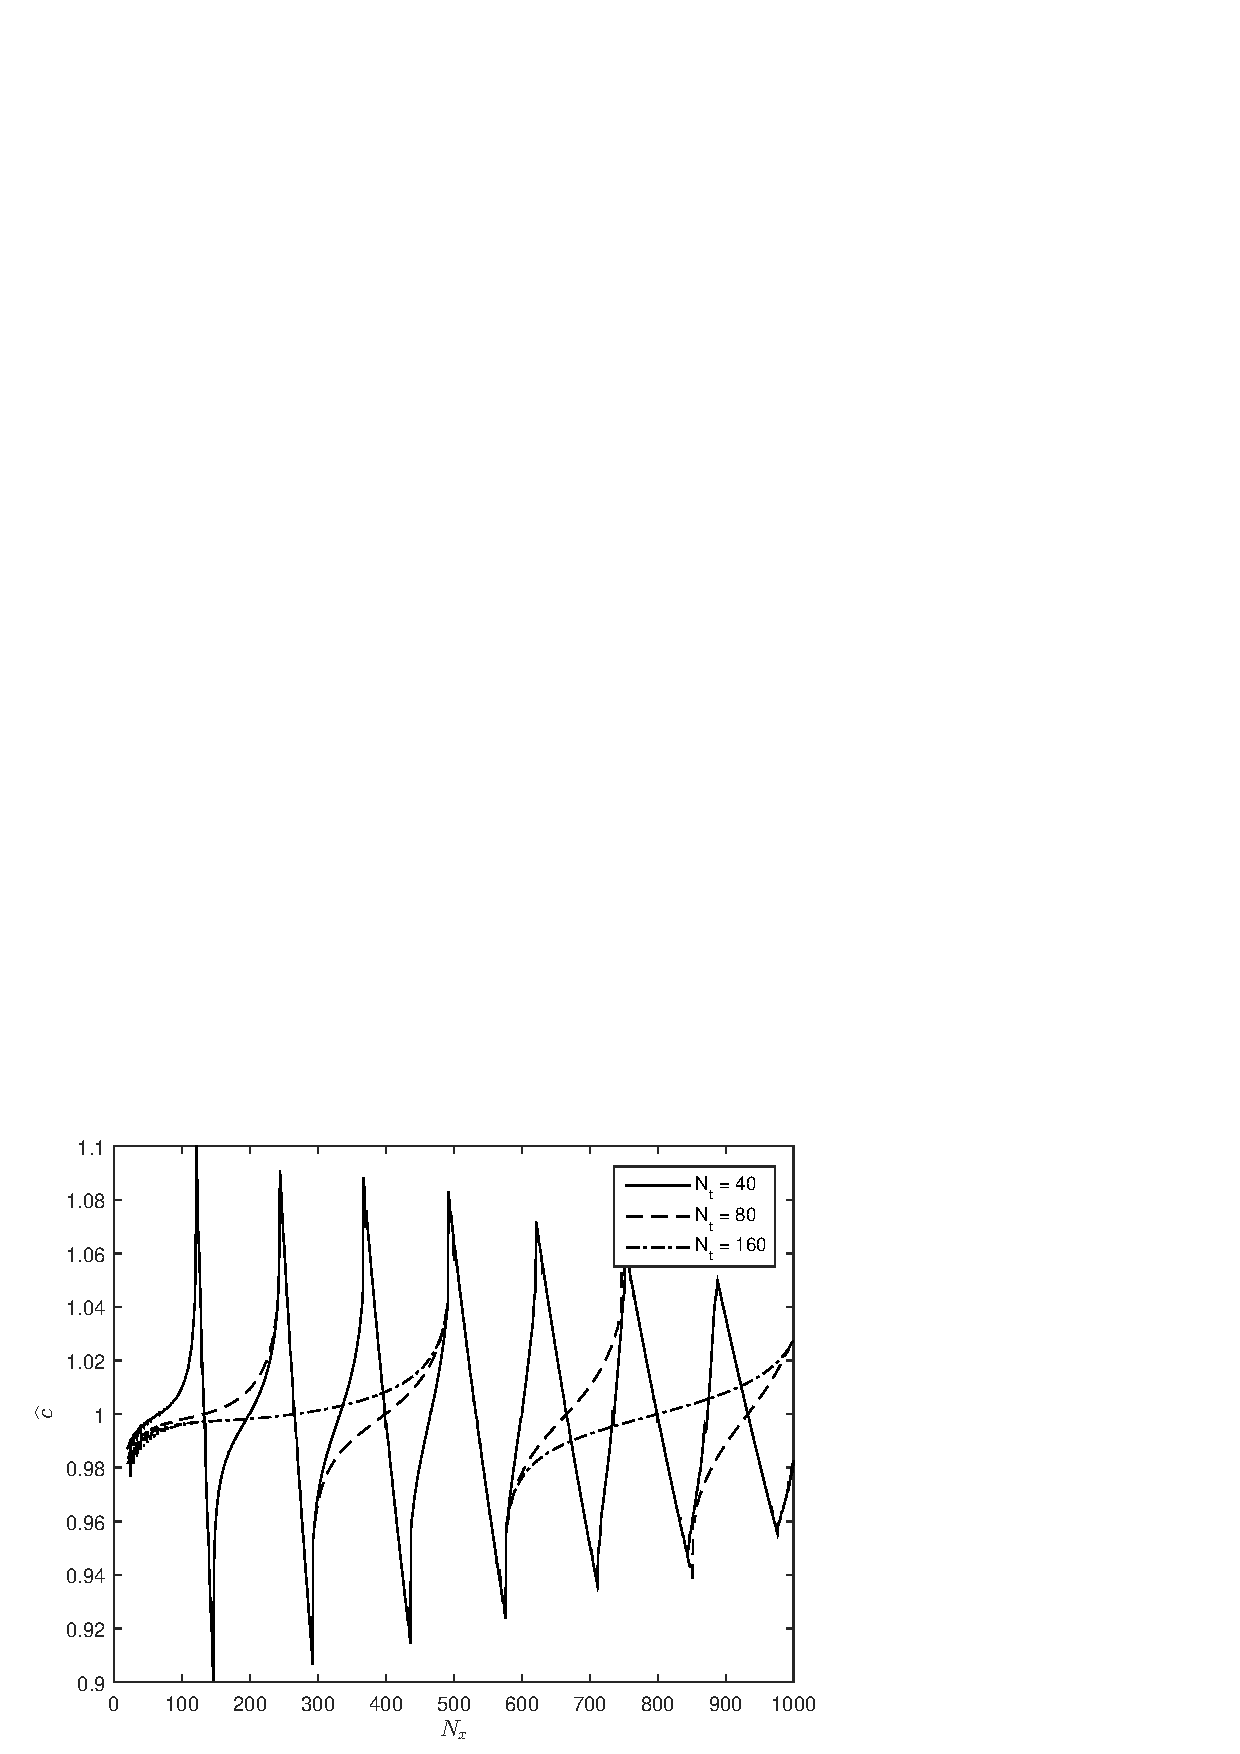
\includegraphics[width=0.9\textwidth]{barry2-k.pdf}
  \caption{Hermite interpolant with Hyman derivative estimates.
  \label{fig:barry2-k}}
\end{figure}
\begin{figure}[htbp]
\centering
  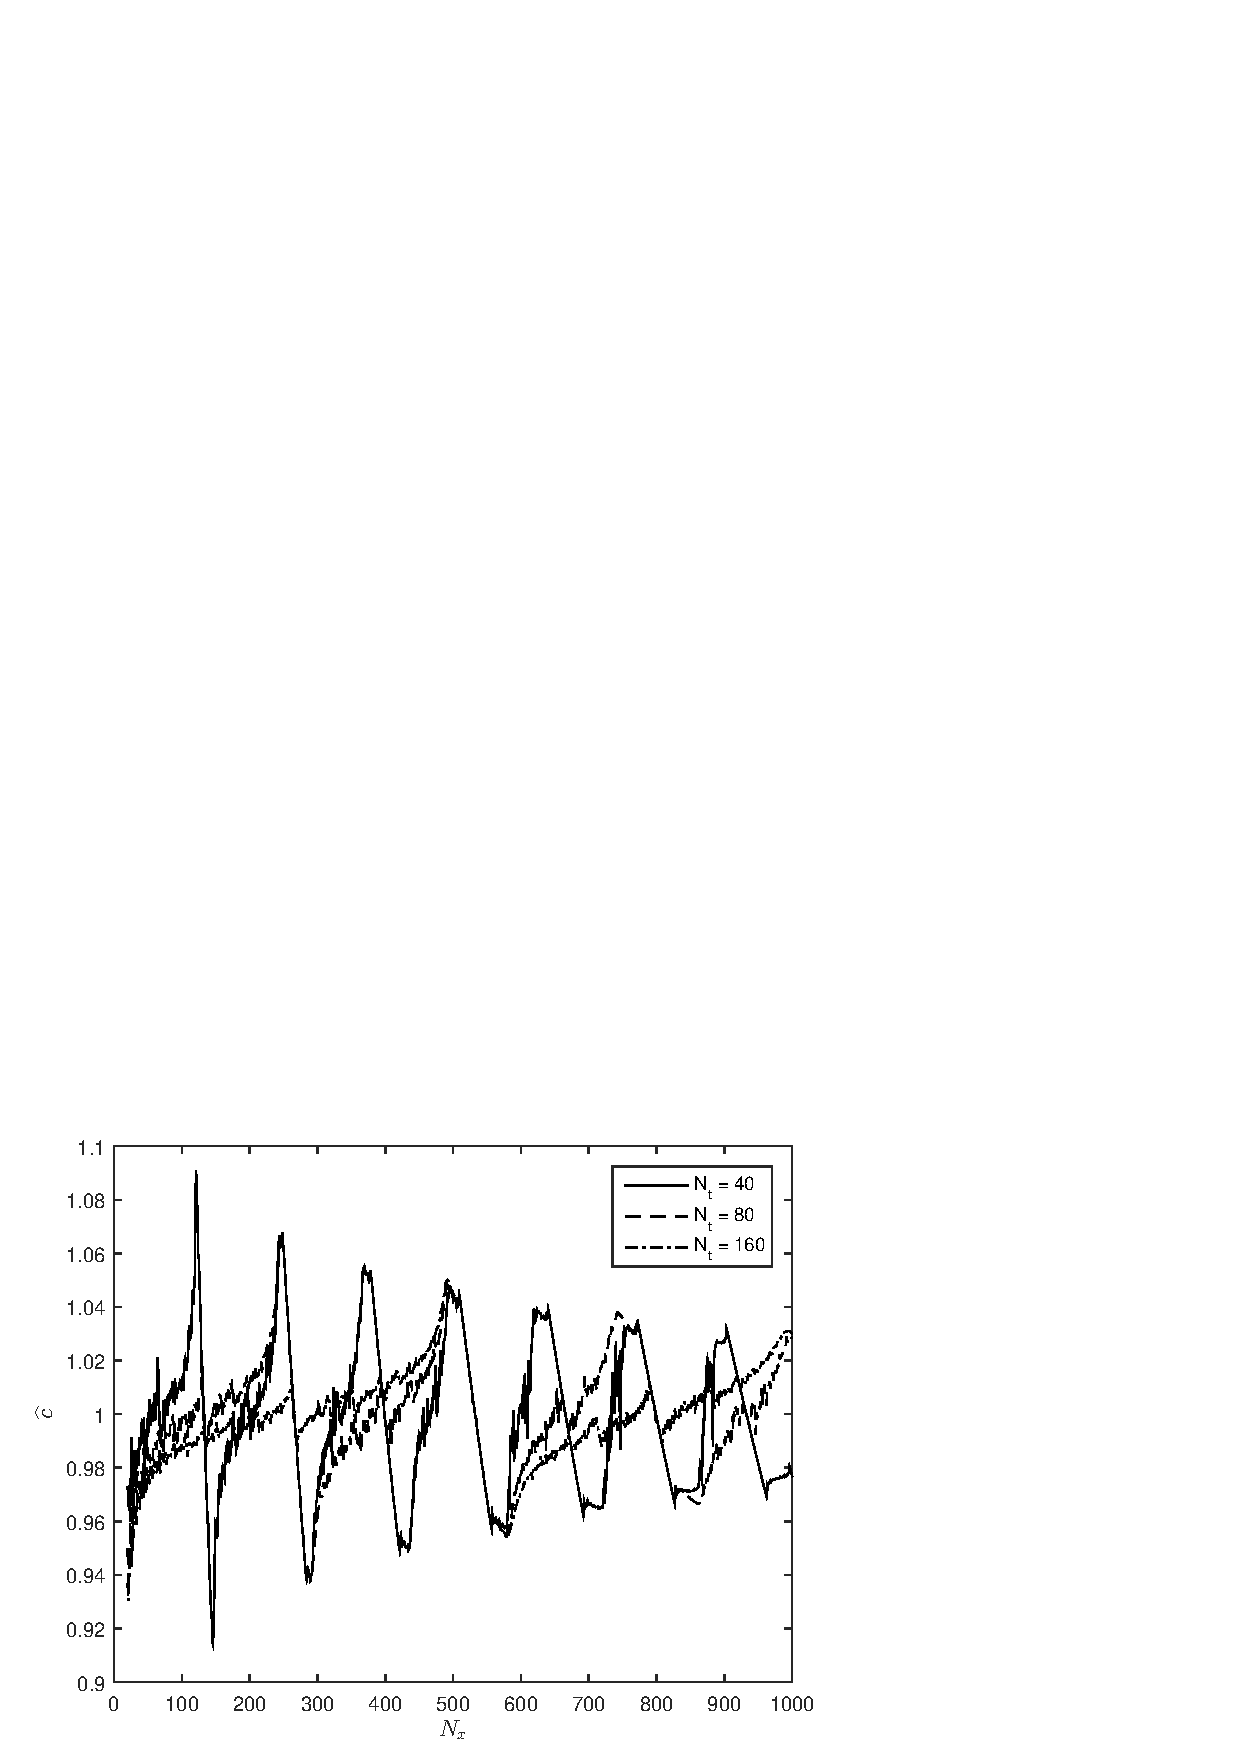
\includegraphics[width=0.9\textwidth]{barry3-k.pdf}
  \caption{ENO interpolant, followed by a flux limiter.
  \label{fig:barry3-k}}
\end{figure}
\begin{figure}[htbp]
\centering
  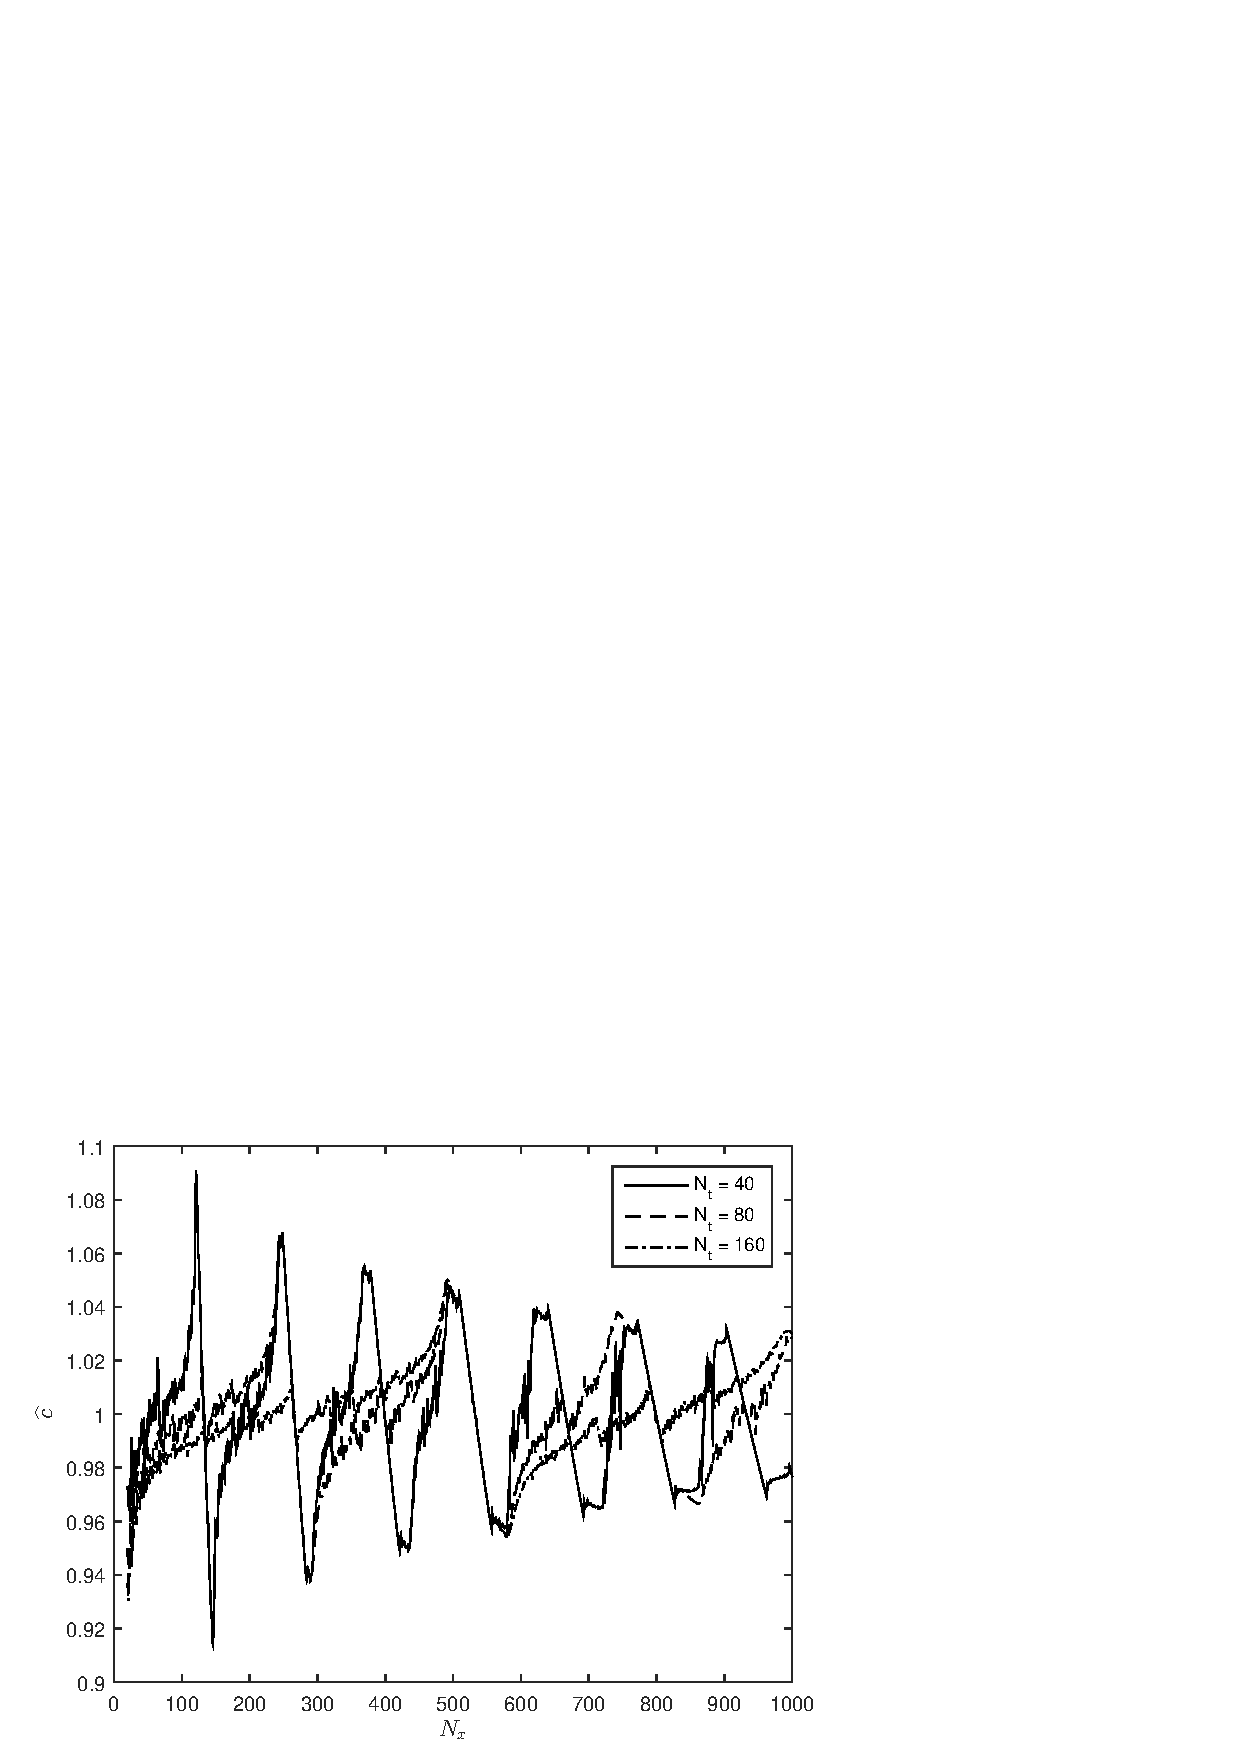
\includegraphics[width=0.9\textwidth]{barry4-k.pdf}
  \caption{ENO interpolant, no flux limiter.
  \label{fig:barry4-k}}
\end{figure}

\clearpage
\section{Numerical results for viscosity}

\begin{figure}[htbp]
\centering
  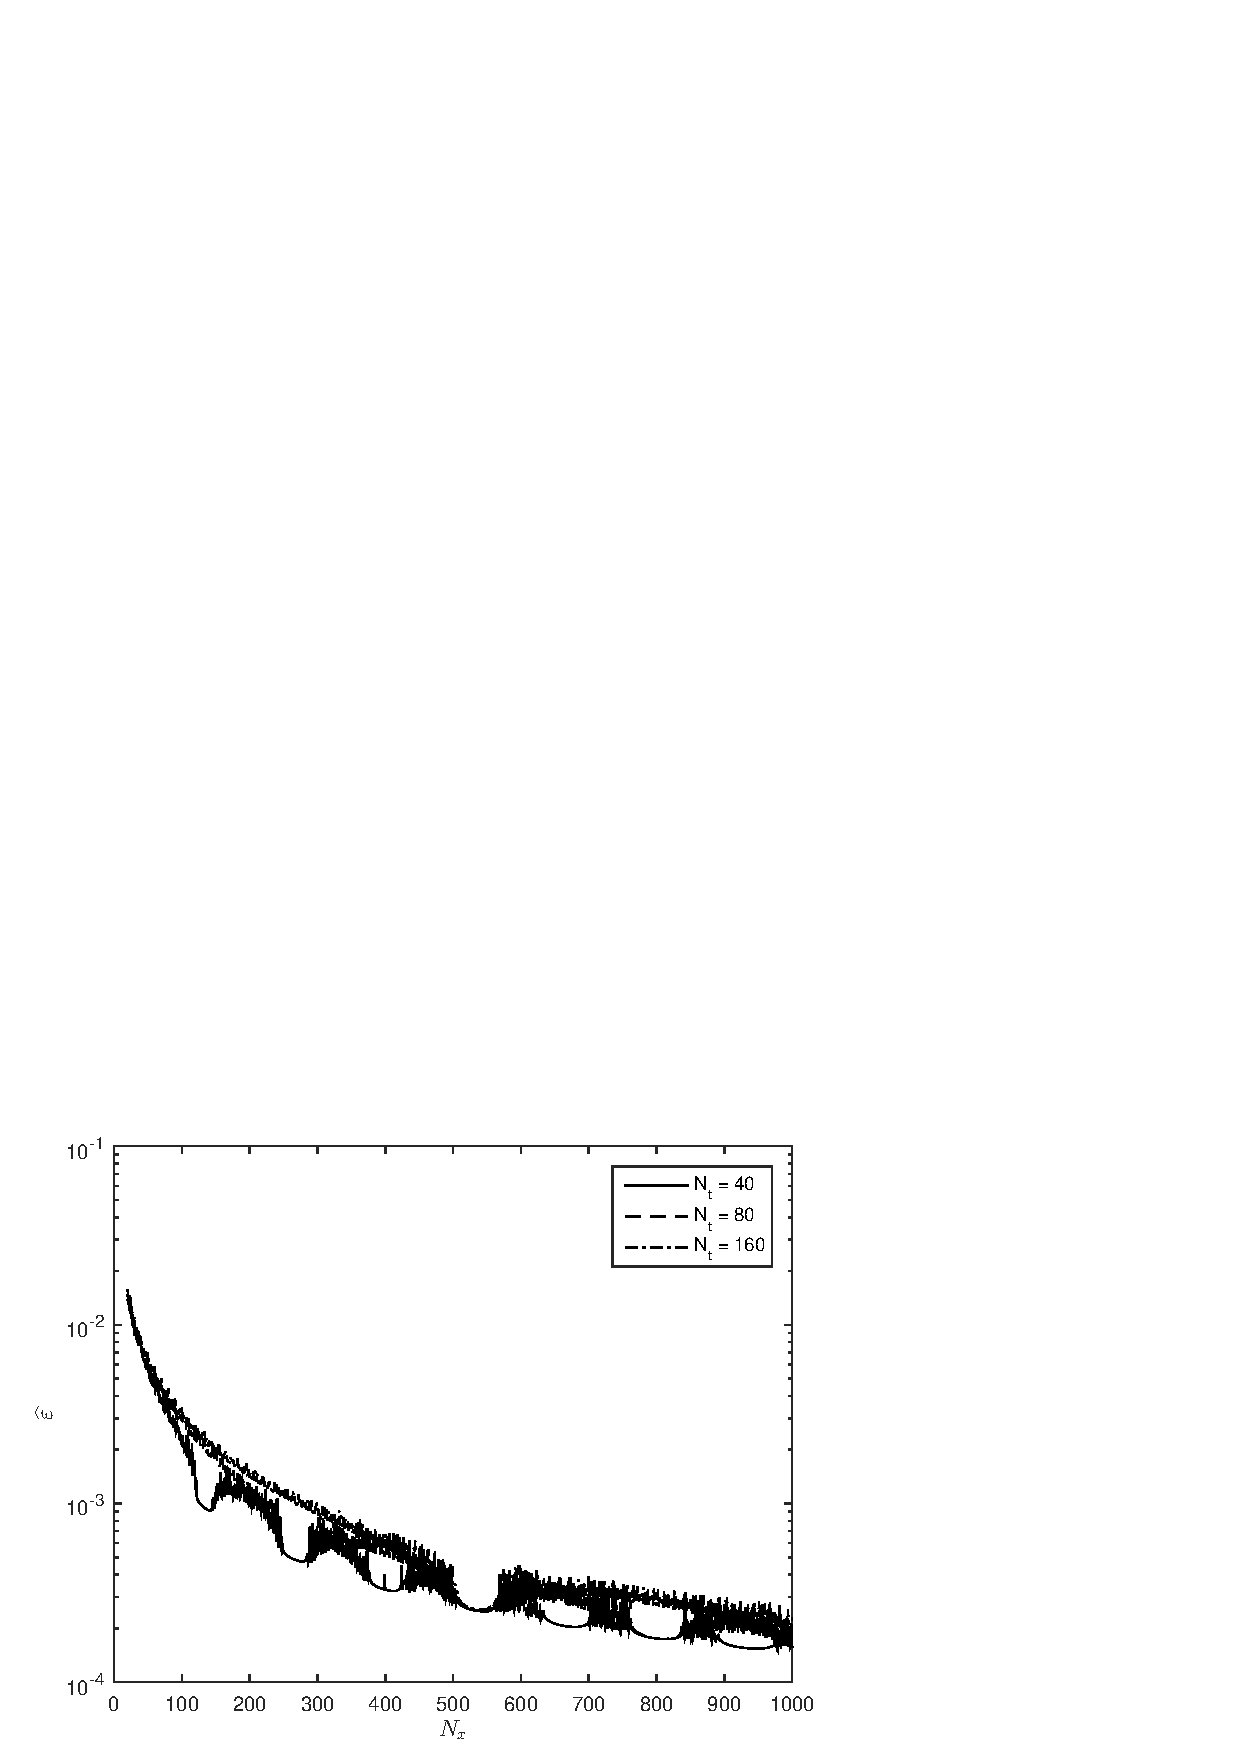
\includegraphics[width=0.9\textwidth]{barry1-eps.pdf}
  \caption{Hermite interpolant with Hyman derivative estimates and guaranteed
    monotonicity.
  \label{fig:barry1-eps}}
\end{figure}
\begin{figure}[htbp]
\centering
  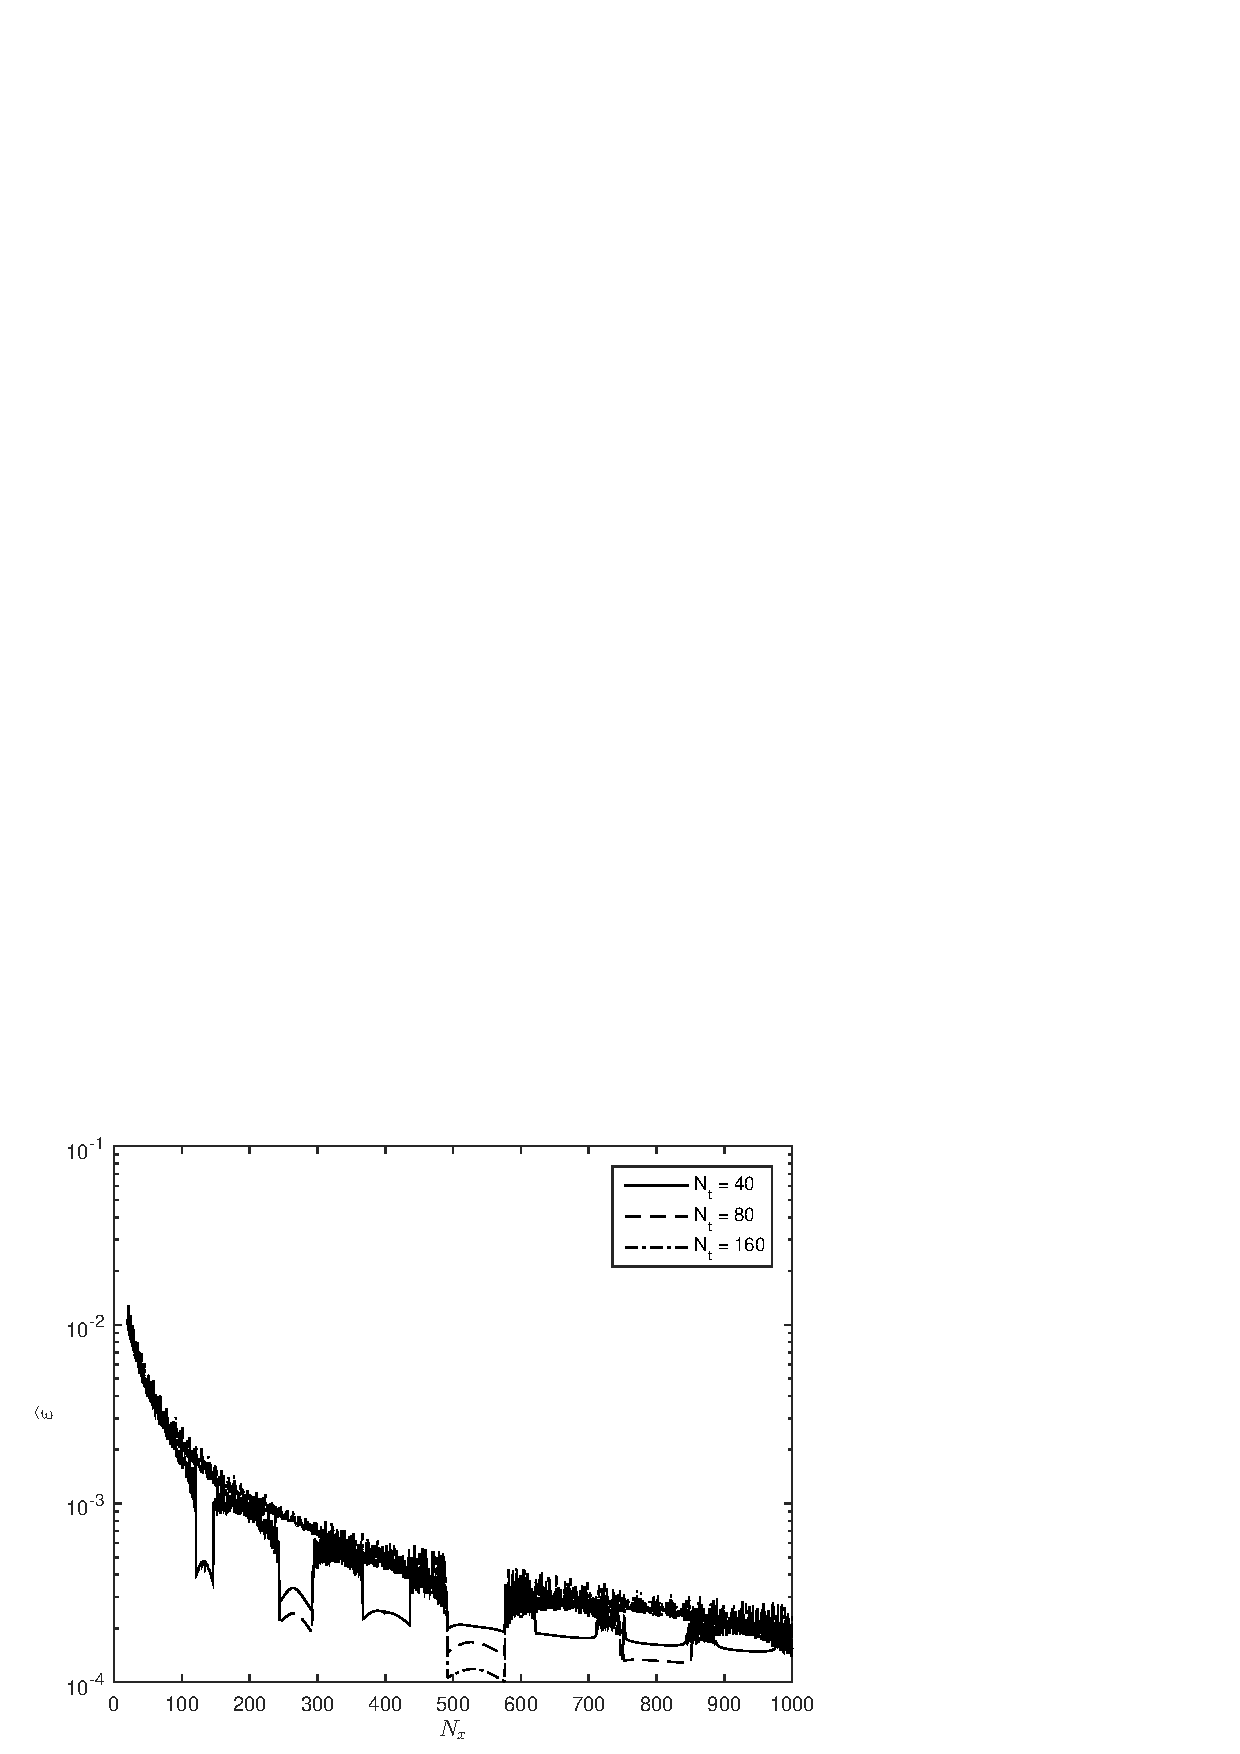
\includegraphics[width=0.9\textwidth]{barry2-eps.pdf}
  \caption{Hermite interpolant with Hyman derivative estimates.
  \label{fig:barry2-eps}}
\end{figure}
\begin{figure}[htbp]
\centering
  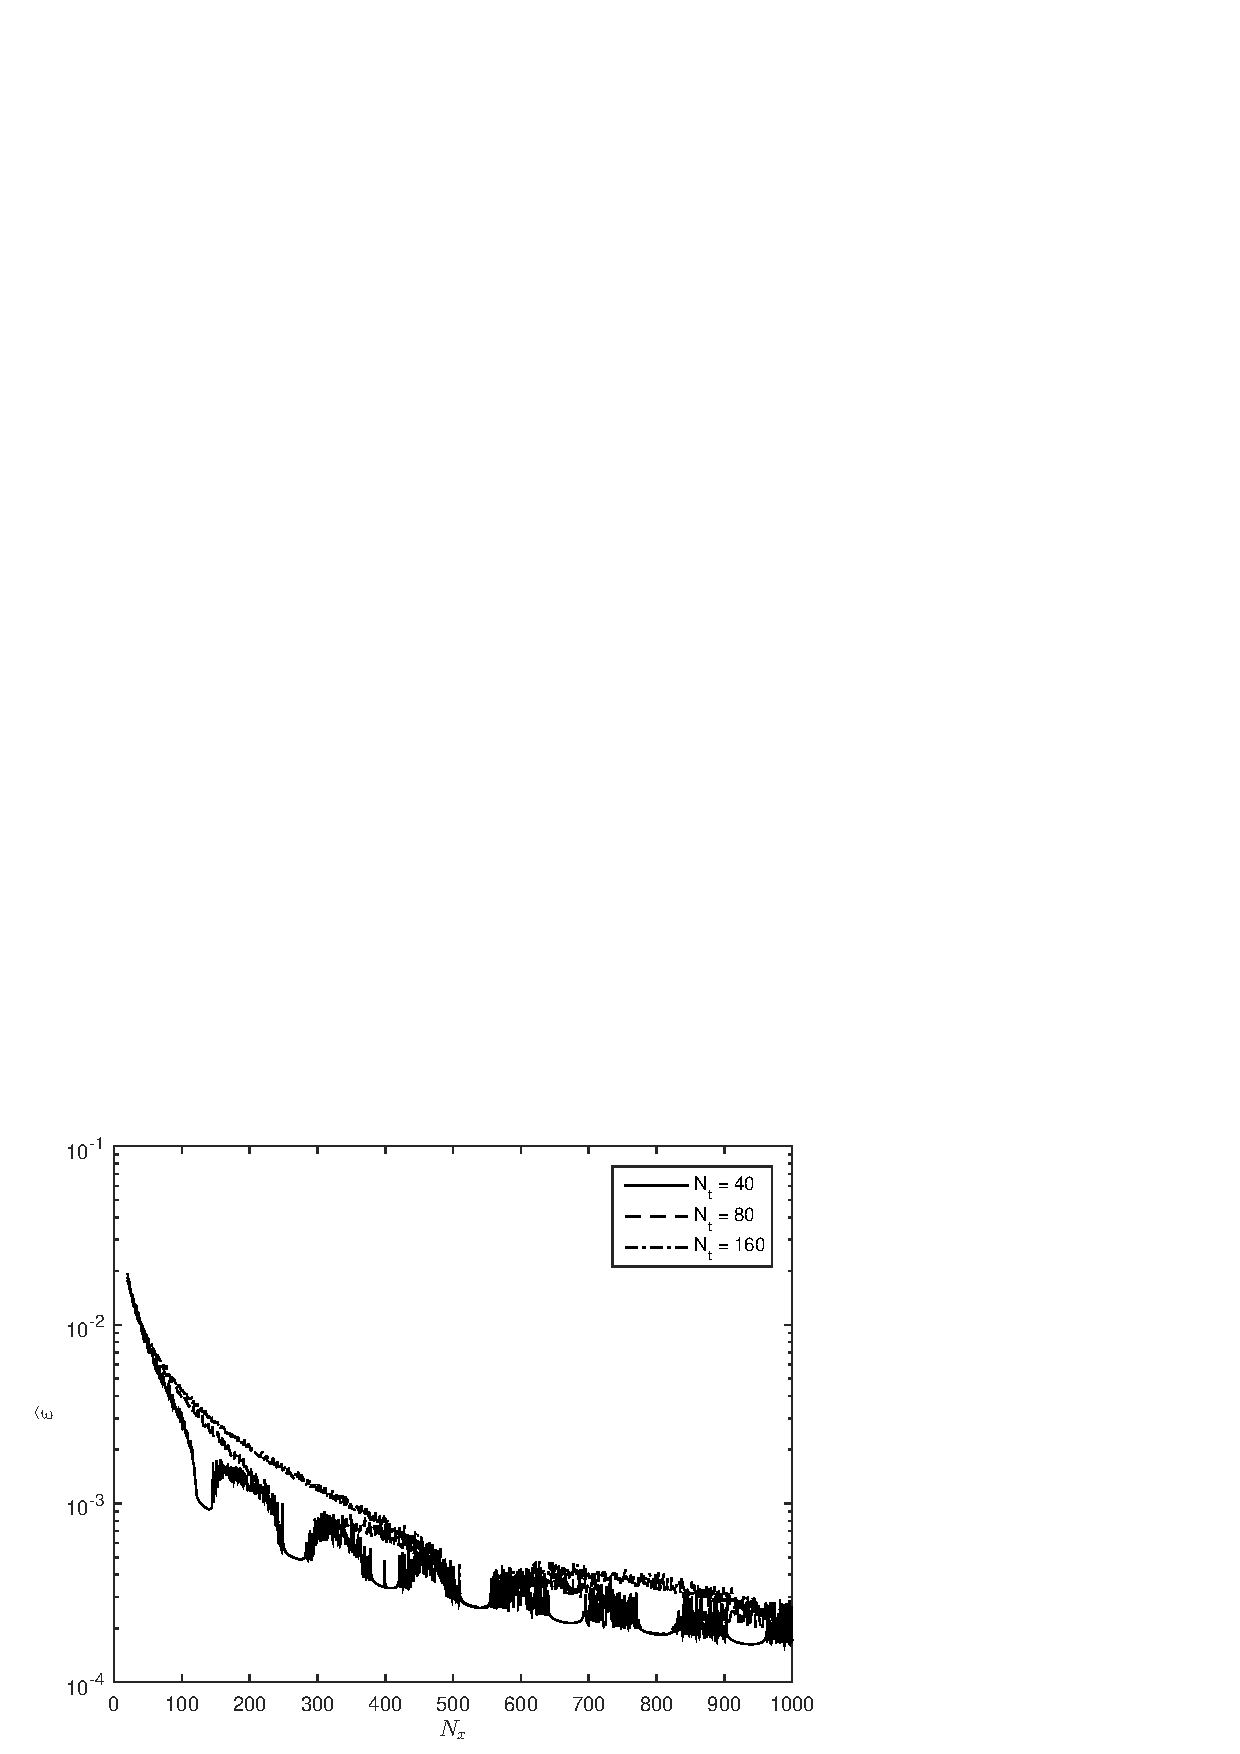
\includegraphics[width=0.9\textwidth]{barry3-eps.pdf}
  \caption{ENO interpolant, followed by a flux limiter.
  \label{fig:barry3-eps}}
\end{figure}
\begin{figure}[htbp]
\centering
  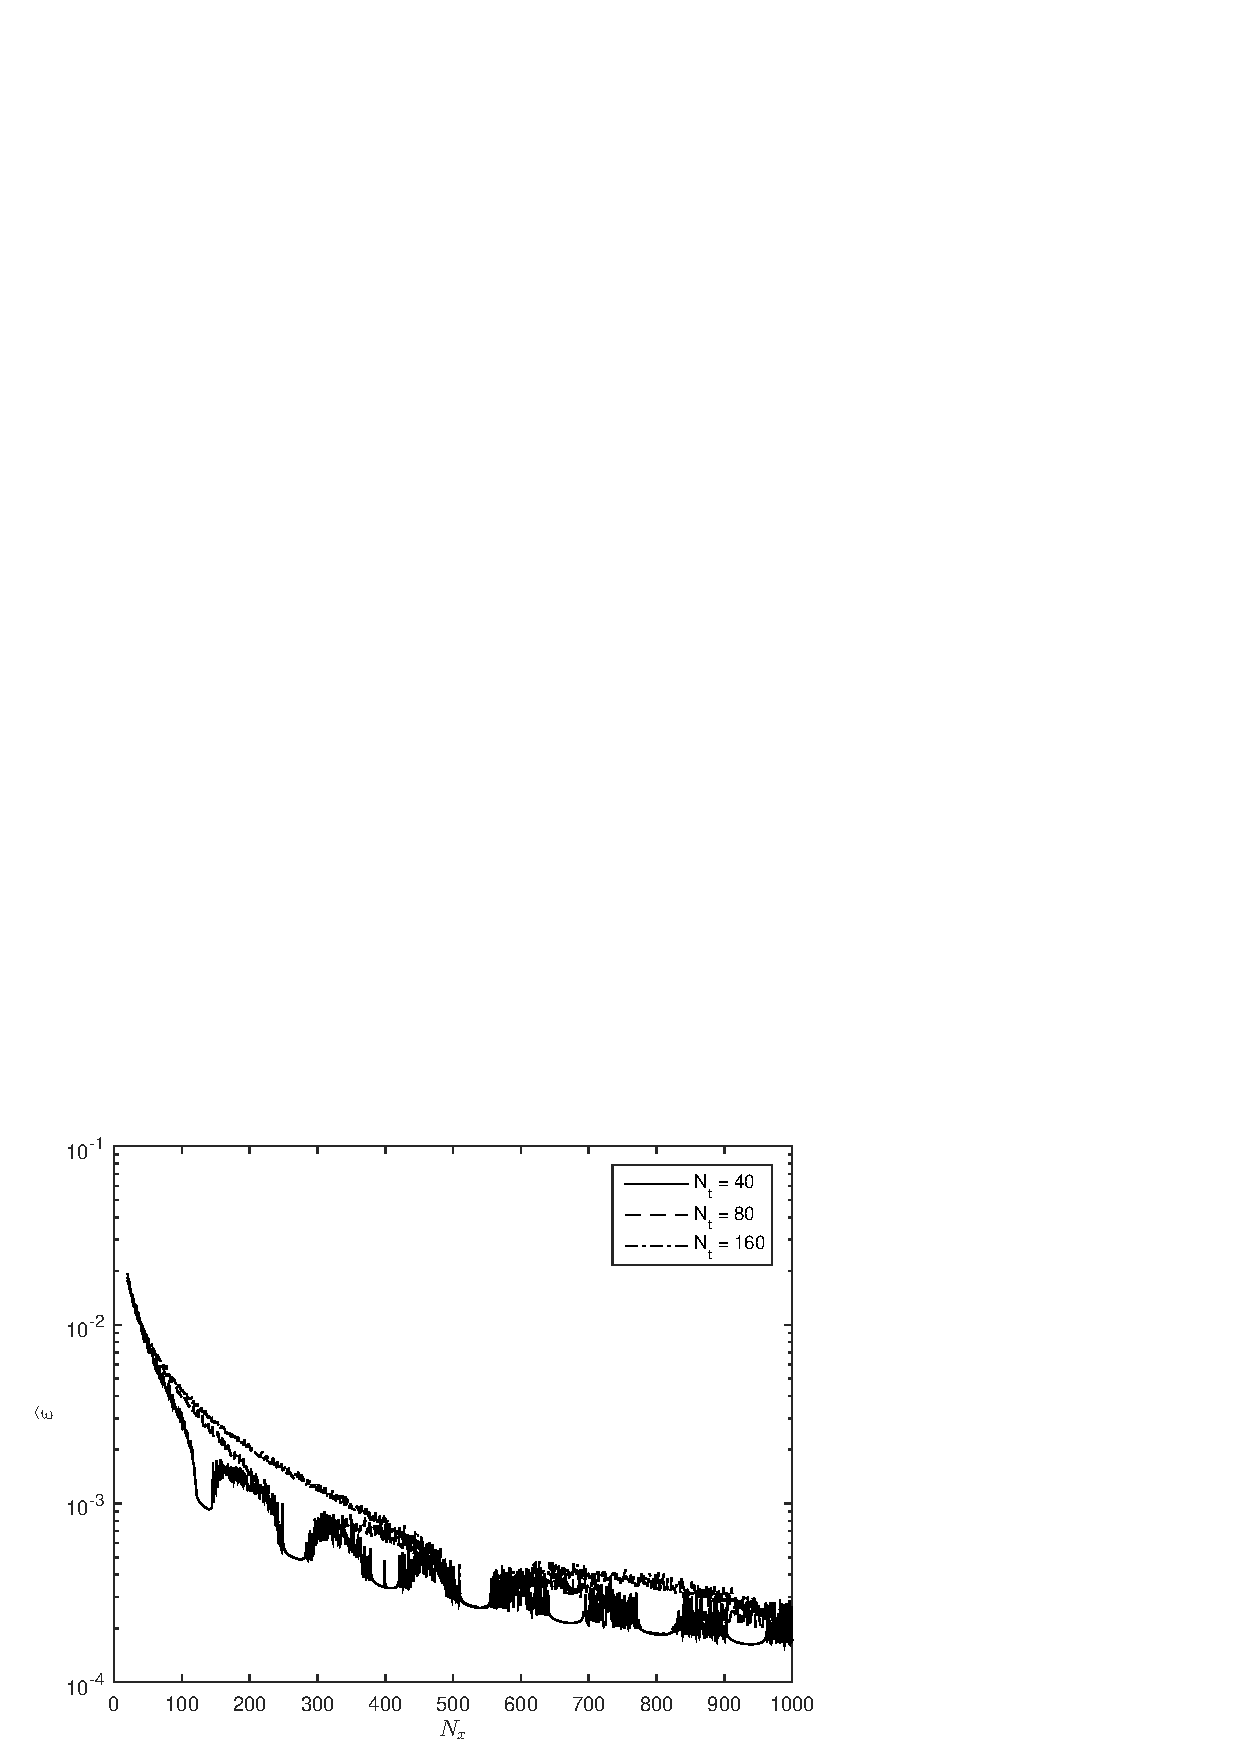
\includegraphics[width=0.9\textwidth]{barry4-eps.pdf}
  \caption{ENO interpolant, no flux limiter.
  \label{fig:barry4-eps}}
\end{figure}

\end{document}
